
\documentclass{gist}


\def\putepsf#1{\centering \parbox{14cm}{\epsfxsize = 14cm \epsfbox{#1}}}
\usepackage{graphicx}

\usepackage{amsmath, amssymb}

% \usepackage{algorithm}
% \usepackage{amsfonts}
% \usepackage{algorithmic}
\AtBeginEnvironment{algorithm}{\setstretch{1.0}}
\usepackage[lofdepth=1]{subfig}
\usepackage[rightcaption]{sidecap}
\usepackage{multirow}
\usepackage{makecell}
% \usepackage{array}

% yoon
\usepackage[ruled,vlined,linesnumbered]{algorithm2e}
\usepackage{etoolbox}
\usepackage{url}

\newcommand\etal{\textit{et~al.\ }}
\newcommand\eg{\textit{e.g.\ }}
\newcommand\ie{\textrm{i.e.\ }}
\newcommand\R{\mathbb{R}}
% yoon

% \usepackage{theorem}
\usepackage{setspace}
\usepackage{appendix}
\usepackage{cite}
\usepackage{csquotes}

% \usepackage{color}
% \usepackage{xcolor}
% \makeatletter
% \let\NAT@parse\undefined
% \makeatother
\usepackage[]{hyperref}
% \hypersetup{
%     bookmarksnumbered=true,
%       linkbordercolor=blue,
%       filebordercolor=red,
%       citebordercolor = green,      
%       urlbordercolor=red,
%       %
%       % colorlinks=true,
%       % linkcolor=blue,
%       % filecolor=blue,
%       % citecolor = blue,      
%       % urlcolor=cyan,
% }

\usepackage{bookmark}
\bookmarksetup{numbered}

\makeatletter
\bookmarksetup{%
  addtohook={%
    \ifnum\toclevel@chapter=\bookmarkget{level}\relax
      \renewcommand*{\numberline}[1]{CHAPTER #1 }%
    \fi
  },
}
\makeatother

\usepackage{cleveref, autonum}

\usepackage{amsthm}
\newtheorem{theorem}{Theorem}[section]
\newtheorem{lemma}{Lemma}[section]
\newtheorem{corollary}{Corollary}[section]
\newtheorem{proposition}{Proposition}[section]
\newtheorem{assumption}{Assumption}[section]
\theoremstyle{remark}
\newtheorem{remark}{Remark}[section]
\theoremstyle{definition}
\newtheorem{definition}{Definition}[section]

%-----------------------------------------------------------------------
% Department code list
% IC - Information and Communications
% IM - Information and Mechatronics
% EC - Electric Engineering and Computer Science
% MS - Materials Science and Engineering
% ME - Mechatronics
% EN - Earth Science and Environmental Engineering
% LS - Life Science
% PH - Physics and Photon Science
% CH - Chemistry
% NA - Nanobio Materials and Electronics
% MD - Biomedical Science and Engineering
% ET - Integrated Technology 에너지 융합 학제
% CT - Integrated Technology 문화기술 융합 학제
% RT - Integrated Technology 지능로봇프로그램

% Department code
%\code{{BS/}{EC}}
%\code{{MS/}{EC}} % 학위와 소속 코드, 초록 페이지에 나타남
\code{{MS/}{ME}}
%-----------------------------------------------------------------------
% Thesis title in English
% Insert \titlebreak where lines are to be separated.  Do not use the LaTeX command '\\'.

%\etitle{Study on Image Segmentation and Action Recognition in Computer Vision}

\etitle{
Constrained Optimization-Based Neuro-Adaptive Control (CoNAC) for Euler-Lagrange Systems
}

%\etitle{Study on Segmentation and Recognition for an Image Understanding}
%\etitle{Genetic Programming: \titlebreak New Optimization Tools for Real-World Applications}

%-----------------------------------------------------------------------
% Thesis title in Korean
% Insert \titlebreak where lines are to be separated.  Do not use the LaTeX command '\\'.
%\begin{spacing}{2.0}
\ktitle{
오일러-라그랑주 시스템을 위한 제약 최적화 기반 신경망 적응 제어
}
%\end{spacing}
%-----------------------------------------------------------------------
% Advisor's name in English without a position such as 'Prof.'.
\advisor{Kyunghwan Choi}

%-----------------------------------------------------------------------
% Advisor's name in Korean without a position such as 'Prof.'.
\kadvisor{최경환}

%-----------------------------------------------------------------------
% Co-advisor's name in English
% In case there is no co-advisor, comment out the following line with a "%" in the front.
%\coadvisor{My Co-advisor}

%-----------------------------------------------------------------------
% Name of the author in English
\ename{Myeongseok Ryu}

%-----------------------------------------------------------------------
% Name of the author in Korean seperated with '{}'.
\kname{{}{}{}{}{유}{명}{석}} % 한글 이름 7글자까지 가능, 오른쪽 끝에 맞춰서 입력

%-----------------------------------------------------------------------
% Student ID of the author
\studentid{20231022}

%-----------------------------------------------------------------------
% The year of graduation (ex. 1999)
\coveryear{2025}

%-----------------------------------------------------------------------
% The date signed by the advisor.  The first is the month, second the date, and third the year.
\advisorsigndate{December}{11}{2024}

%-----------------------------------------------------------------------
% The date signed by the referees.  The first is the month, second the date, and third the year.
\refereesigndate{December}{11}{2024}

%-----------------------------------------------------------------------
% Names of the referees in English
% For Master's thesis, input the names of the three referees (refereeA thru referee C) in full.
% For Ph.D thesis, input the names of the five referees (refereeA thru referee E) in full.
% For most cases, refereeA is the same as the advisor.

\refereeA{Prof. Kyunghwan Choi.}
\refereeB{Prof. Hyo-Sung Ahn.}
\refereeC{Prof. Pilwon Hur.}
% \refereeD{Prof. fourth prof.}
% \refereeE{Prof. fifth prof.}

%-----------------------------------------------------------------------
% This is the beginning of the thesis.

\dedication{
Dedicated to my family.
}

\begin{document}
%-----------------------------------------------------------------------
% Abstract of the thesis in English.
% Insert the abstract between \begin{eabstract} and \end{eabstract}.
% You can either write the abstract directly here or import a file using the \input command.

%%%%%%%%%%%%%%%%%%%%%%%%%%%%%%%%%%%%%%%%%%
% Abstract by English
%%%%%%%%%%%%%%%%%%%%%%%%%%%%%%%%%%%%%%%%%%

\begin{eabstract}
\begin{spacing}{2.0} % double spacing

%%%%%%%%%%%%%%%%%%%%%%%%%%%%%%%%%%%%%%
% Abstract of the thesis in English
%%%%%%%%%%%%%%%%%%%%%%%%%%%%%%%%%%%%%%

This thesis presents a constrained optimization-based neuro-adaptive controller (CoNAC) for uncertain Euler-Lagrange systems subject to weight norm and input constraints. 
A deep neural network (DNN) is employed to approximate an ideal stabilizing control law which compensates for lumped system uncertainties while addressing both types of constraints. 
The weight adaptation laws are derived from constrained optimization theory, ensuring first-order optimality conditions at steady state. 
The controller’s stability is rigorously analyzed using Lyapunov theory, ensuring bounded tracking errors and DNN weights. 
Two numerical simulations were constructed to compare CoNAC with other benchmark controllers.
The simulations demonstrated effectiveness of CoNAC in tracking error regulation and satisfaction of constraints.



\end{spacing}
\end{eabstract}

%-----------------------------------------------------------------------
% Abstract of the thesis in Korean.
% Insert the abstract between \begin{kabstract} and \end{kabstract}.
% You can either write the abstract directly here or import a file using the \input command.

%%%%%%%%%%%%%%%%%%%%%%%%%%%%%%%%%%%%%%%%%%
% Abstract by Korean
%%%%%%%%%%%%%%%%%%%%%%%%%%%%%%%%%%%%%%%%%%

\begin{kabstract}
\begin{spacing}{2.0} % double spacing

%국문초록
%%%%%%%%%%%%%%%%%%%%%%%%%%%%%%%%%%%%%%
% Abstract of the thesis in Korean
%%%%%%%%%%%%%%%%%%%%%%%%%%%%%%%%%%%%%%

본 논문은 신경망 가중치와 제어 입력의 제약 조건이 있는 불확실한 오일러-라그랑주 시스템을 위한 제약 최적화 기반 신경망 적응 제어기를 제안한다.
깊은 신경망은 부여된 두 제약조건을 만족하는 동시에 시스템의 불확실성을 보상하며 원하는 제어 법칙을 근사하도록 사용되었다.
가중치의 적응 법칙은 제약 최적화 이론으로 부터 유도되었으며, 정상 상태에서 1차 최적성 조건을 만족시킨다.
제어기의 안정성은 리아푸노프 이론을 사용하여 분석되었으며, 추종 오차와 신경망 가중치의 크기가 제한됨을 보여준다.
제안된 제어기를 다른 벤치마크 제어기와 비교하기 위해 두 개의 시뮬레이션이 시행되었다.
시뮬레이션을 통하여 추종 성능과 제약 조건 만족에 제안된 제어기가 다른 제어기에 비하여 좋은 지표를 가진다는 것을 보였다.

\end{spacing}
\end{kabstract}


%-----------------------------------------------------------------------
% Table of contents, list of tables and list of figures.
% Use the \makecontents command to automatically generate the table of content
\makecontents

% In case there is no table, comment out the following line.
% \listtables

% In case there is no figure, comment out the following line.
\listfigures

% In case there is no algorithm, comment out the following line.
% \listalgorithms

%-----------------------------------------------------------------------
% Input the thesis files written in LaTeX.
% The \begin{document} command is not necessary here.
% Refererence and vitae will folllow the main thesis text.
%-----------------------------------------------------------------------
% This is the beginning of the main thesis body.
% Insert Chapter or section or subsection as many as you need.

%%%%%%%%%%%%%%%%%%%%%
% Chapter 1 Introduction
%%%%%%%%%%%%%%%%%%%%%

%%%%%%%%%%%%%%%%%%%%%%%%%%%%%%%%%%%%%%
% DO NOT DELETE FOLLOWING TWO LINES! %
%%%%%%%%%%%%%%%%%%%%%%%%%%%%%%%%%%%%%%
% \begin{spacing}{2.0} % double spacing
\begin{spacing}{1.3} % double spacing
\pagenumbering{arabic}
\setcounter{page}{1}

% you start with the chapter 1

%%%%%%%%%%%%%%%%%%%%%%%%%%%%%%%%
% Chap 1. Introduction
%%%%%%%%%%%%%%%%%%%%%%%%%%%%%%%%

\chapter{Introduction}

\section{Background} 

\subsubsection{Neural Networks in Control Design}

Recent advances in deep learning field have shown that neural networks (NNs) can be used in a wide range of applications. 
A fundamental idea of deep learning is to utilize the well-known universal approximation capability of the NNs, which allows them to approximate any smooth function over a compact set with minimal approximation error. 
Using this property, various architectures of NNs have been introduced such as convolutional neural networks (CNNs) for image processing, recurrent neural networks (RNNs) for time-series data, and long short-term memory (LSTM) networks for sequential data. 
These advances have motivated many researchers in the control field to leverage NNs for control design.
 
In general, the NNs are used in control design as a parameter estimator or controller.
In other words, the NNs are trained to produce corresponding output to certain input (\eg real system parameters or desired control input from current system output).
Hence, designers need to make a dataset which contains input-output pairs, to train the NNs.
Random control inputs are typically applied to collect the input-output pairs by exploring the interested operating domain.
Then, the NNs are trained to approximate the input-output mapping using the dataset via supervised learning methods to solve regression problem.
For example, as the parameter estimators, 1-Dimensional convolutional neural network (1D-CNN) is used for friction potential estimation \cite{RN109}.
Similarly, CNN is used to estimate the road conditions (\eg dry or icy condition) by extracting features of road image from built-in camera \cite{RN118}.
A time delay neural network (TDNN) is used to estimate tire-road friction coefficient for vehicle control \cite{RN107}.
In addition, for motor systems, specific architectures of NNs are used to estimate for the nonlinearity of voltage source inverter and synchronous machine \cite{RN115}.

On the other hand, as the controller, the NNs are trained to imitate given desired control input.
Thus, designers should design desired controller as the output of input-output pair for training as well.
In \cite{RN117, RN116}, CNNs are used to produce steering angle from raw pixel data of camera for vehicle control.
This literature shows that end-to-end controller can be achieved by using NNs. 
As an optimal feedforward torque control of synchronous machines, NNs are used to produce optimal reference current \cite{RN112, RN113, RN114} which is calculated using nonlinear programming (NLP).
The literature reported that the NNs can provide the optimal reference current with less computational cost than existing methods.
This is because, in general, NLP needs high computational cost to solve the optimization problem exhibiting unsuitability for real-time control.
In contrast, once the NNs are trained, they can be used for real-time control, since they consist of simple matrix affine operations and element-wise nonlinear functions.
Especially, in \cite{RN114}, multi-objective hyperparameter optimization is utilized to obtain optimal structure of NN regarding floating point operations (FLOPS) which can be considered as computational cost, and current errors, since motor systems require high frequency of control input.

In conclusion, if the NNs are well-trained, the NNs can be used as an estimator or controller in the control system, with smaller computational cost (if online-train is not conducted) and sufficient accuracy.
However, if an operating point goes outside the interested operating domain, the NNs can not provide the accurate estimation or control input.
This is because, the NNs are train through the dataset which is collected in the interested operating domain (\ie they are trained for interpolation not extrapolation of the dataset).
Furthermore, the NNs are inherently black-box models whose input-output mapping is not interpretable \cite{RN16, RN17}.
This causes stability and safety problems of the system, since the possibility of unexpected behavior (\eg excessively large or non-proper control input) of the controller exists.
Therefore, the stability analysis of the control system with NNs should be conducted to ensure the stability and safety in a perspective of control theory.

\subsubsection{Neuro-Adaptive Control}

From 1980s, as a branch of adaptive control, neuro-adaptive control (NAC) has been developed to leverage the NNs for control design to approximate unknown system dynamics or entire control laws \cite{RN5, RN48}.
The conventional adaptive control is a control method that adapts the control parameters to compensate for uncertainties in the system dynamics, since, in practice, real systems often contains uncertainties due to unmodeled dynamics, parameter variations, or external disturbances which can significantly degrade control performance and lead to instability. 
Similarly, NAC methods approximate the uncertainties via NNs and adapts the weights of the NNs.
For more details of conventional adaptive control, the reader is referred to \cite{RN6, RN10}. 

The adaptive control methods typically ensure the stability of the control system including adaptation law, in the sense of Lyapunov by conducting Lyapunov stability analysis or deriving adaptation law using Lyapunov stability analysis.
As a branch of adaptive control, the adaptation laws of NAC methods also ensure the stability. 
This means that the NAC methods have online adaptation (train) capability with stability guarantees. 
It is notable, that the adaptation laws of NAC methods (which will be presented in the Section \ref{chap1:sec:example} with a simple example) use the current observed error as the feedback signal to be backpropagated for adaptation (\ie generally it is prediction error of NNs). 
Since the NN’s weights are adapted according to current observed error which is dependent on current NN’s weights, the offline adaptation methods can not be conducted. 
This feature makes NAC methods be more close to reinforcement learning methods which attempts to maximize expectation value of reward (\ie reward is typically defined as sign changed tracking error.) and need to implemented in real-time to obtain current reward.

Besides, since NAC is based on control theory, relatively simpler NN architectures and adaptation methods are used due to their brief mathematical expression.
Most widely utilized architectures are single hidden layer neural networks (SHLNNs) \cite{RN69, RN18, RN85, RN46, RN95, RN108} and radial basis function neural networks (RBFNNs) \cite{RN89, RN82, RN64, RN71, RN19, RN21}.
Recently, deep NNs (DNNs) are utilized in NAC with stability guarantees \cite{RN13}.
The DNNs are more effective for complex system approximation than shallow NNs, since it offer greater expressive power with same number of neurons \cite{RN65}.
Additionally, variations of DNNs, such as long short-term memory (LSTM) networks for time-varying dynamics \cite{RN11} and physics-informed neural networks (PINNs) for leveraging physical system knowledge \cite{RN12}, have further extended the capabilities of neuro-adaptive control systems.

These various NNs are typically employed to improve the conventional control methods.
In \cite{RN69, RN95}, the NNs are used to compensate for system uncertainties in the feedback linearization control.
Similarly, the NNs are used to approximate the unknown dynamics in the backstepping control for higher-order system in \cite{RN85, RN19, RN71, RN80}.
Besides, sliding mode control (SMC), impedance control and admittance control are also developed with NNs in \cite{RN64}, \cite{RN89} and \cite{RN82}, respectively.
A few of the NAC methods are utilized NNs to approximate the entire control law \cite{RN46}.
Aforementioned NAC methods have shown the effectiveness of the NNs in control design to approximate system uncertainties and control law.

However, there are some limitations in the existing NAC methods.
In following sections, the limitations are presented, and the research objective is suggested.

\section{Simple Example of Neuro-Adaptive Control} \label{chap1:sec:example}

In this section, a simple example of neuro-adaptive control (NAC) is presented.
Consider a control affine system as follows:
\begin{equation}
    \dot x = f(x) + h(u)
\end{equation}
where $x \in \R^n$ is the state, $f:\R^n\to\R^n$ is the unknown dynamics, $h:\R^n\to\R^n$ is control input saturation function, and $u \in \R^n$ is the control input.
The objective of this control problem is to design a control law $u$ such that the state $x$ converges to the origin.
The unknown dynamics $f(x)$ can be approximated via NNs according to the universal approximation theorem presented in Theorem \ref{chap2:thm:uni_approx}, as follows:
\begin{equation}
    f(x) = \Phi(x;\theta^*) + \epsilon
\end{equation}
where $\Phi(\cdot)$ denotes a universal approximator (\eg SHLNNs, RBFNNs or DNNs), $\theta^*$ is the ideal weight and $\epsilon$ is the approximation error.
Note that $\theta^*$ is supposed to be constant ($\dot\theta^*=0$) and bounded.

Ignoring control input saturation, a desired feedback-linearization based stabilizing control law can be developed as follows:
\begin{equation}
    u^* = -\Phi(x;\theta^*) - \epsilon - k x
\end{equation}
where $k$ is a positive control gain. 
Using the estimation of ideal weight $\hat\theta$, the control law can be approximated as follows:
\begin{equation}
    u = -\Phi(x;\hat\theta) - k x
\end{equation}
where $\hat\theta$ is the estimated weight.
The closed-loop dynamics can be described as follows:
\begin{equation}
    \dot x = \Phi^*+\epsilon + h(-kx-\hat\Phi )
\end{equation}
where $\Phi^* = \Phi(x;\theta^*)$ and $\hat\Phi = \Phi(x;\hat\theta)$.

The adaptation law can be derived based on the Lyapunov stability analysis.
To simplify the derivation, ignore the control input saturation.
Then, taking the time derivative of the Lyapunov function candidate $\mathcal V = (1/2)x^Tx+(1/2\alpha)\tilde\theta^T\tilde\theta$ where $\tilde\theta\triangleq \hat\theta-\theta^*$ and $\alpha\in\R_{>0}$ denotes adaptation gain (learning rate), yields:
\begin{equation}
    \begin{aligned}
        \dot{\mathcal V}
        =& x^T ( - kx + \Phi^* - \hat\Phi + \epsilon ) + {1\over\alpha}\tilde\theta^T \dot{\tilde\theta}
        \\
        =& - k x^Tx + x^T(\Phi^* - \hat\Phi + \epsilon) + {1\over\alpha}\tilde\theta^T \dot{\hat\theta}
        \\
        =& - k x^Tx + x^T( -{\partial \hat\Phi\over\partial \hat\theta}\tilde\theta + \mathcal O(\Vert\tilde\theta\Vert^2) +\epsilon) + {1\over\alpha}\tilde\theta^T \dot{\hat\theta}
        \\
        =& - k x^Tx +\tilde\theta^T
        \bigg(
            {1\over \alpha} \dot{\hat\theta} - {\partial \hat\Phi\over\partial \hat\theta}^T x
        \bigg)
        + x^T\Delta
    \end{aligned}
\end{equation}
where $\mathcal O (\Vert\tilde\theta\Vert^2)$ is the higher order term, and $\Delta\triangleq \mathcal O(\cdot)+\epsilon$ is the lumped disturbance term.
Assuming that $\Delta$ is sufficiently small, the adaptation law which realizes $\dot{\mathcal V}\approx -kx^Tx<0$ can be derived as follows:
\begin{equation}
    \dot{\hat\theta} = \alpha {\partial \hat\Phi\over\partial \hat\theta}^T x
    .
\end{equation}
However, $\Delta$ can dominate the system when an initial (or on certain domain) estimation error $\tilde\theta$ is large.
In result, the parameter drift can occur due to $\Delta$ (\ie the parameter estimation $\hat\theta$ increases to infinity over time (see \cite{RN6})).
In practical physical applications, the parameter drift is crucial since it makes the control input reach to limitation of actuators (\ie the amplitude of control input is dependent on weights).
This can destruct the system performance and lead to the system instability.

\section{Research Objective} \label{chap1:sec:research objective}

To address the above issues (boundedness of weights and control input saturation), constrained optimization offers a promising approach. 
By formulating the NAC problem as an optimization problem with constraints, it is possible to adapt the NN weights (minimize an objective function (e.g., tracking error)) satisfying the constraints regarding with both weight boundedness and control input saturation. 
Constrained optimization provides a theoretical framework for defining optimality of the problem and presents numerical methods for finding solutions \cite{RN9}.
To the best of the authors’ knowledge, no prior work has applied constrained optimization theory to adaptive control systems with real-time weight adaptation.
Only a few of literature are introduced constrained optimization based methods to train NNs more efficiently \cite{RN62, RN98, RN94}.

This gap suggests that constrained optimization could be key to addressing both weight norm boundedness and input constraints in a unified, theoretically grounded framework, particularly in real-time NAC.
In summary, the objective of this thesis is to develop a NAC that can ensures boundedness of the weights and satisfaction of the input saturation via optimization method.

\section{Outline of the Thesis} 

The remainder of this thesis is organized as follows. 
Preliminaries for the thesis are presented in Chapter \ref{chapter2}.
Using the preliminaries the proposed constrained optimization-based neuro-adaptive controller (CoNAC) is presented over Chapter \ref{chapter3} and Chapter \ref{chapter4}.
Each chapter, at first, introduces the exiting methods concerning weight boundedness, and input saturation respectively.
Then, the details of the proposed CoNAC are presented, and simulation results are reported.
Finally, Chapter \ref{chapter5} concludes the thesis and suggests future work.


\end{spacing}

%%%%%%%%%%%%%%%%%%%%%%%%%%%%%%%%%%%%
% Chapter 2 
%%%%%%%%%%%%%%%%%%%%%%%%%%%%%%%%%%%%

% \begin{spacing}{2.0} % double spacing
\begin{spacing}{1.3} % double spacing
%%%%%%%%%%%%%%%%%%%%%%%%%%%%%%%%
% Chap 2. Preliminaries
%%%%%%%%%%%%%%%%%%%%%%%%%%%%%%%%

\chapter{Preliminaries} \label{chapter2}

This chapter presents the necessary background and mathematical tools required for the subsequent chapters.
Since the proposed controller (constrained optimization-based neuro-adaptive controller (CoNAC)) is based on adaptive control and constrained optimization theory and deep neural networks (DNNs), this chapter covers the following topics: control theory, constrained optimization theory, and the approximation theory.

%%%%%%%%%%%%%%%%%%%%%%%%%%%%%%%%
\section{Related Control Theory} \label{chap2:sec:ctrl}
%%%%%%%%%%%%%%%%%%%%%%%%%%%%%%%%

% \subsection{Backstepping Control} \label{chap2:sec:BSC}

In this thesis, the Euler-Lagrange systems will be used as target system since many engineering systems can be modeled using Euler-Lagrange systems (\eg aerospace, robotics, and automotive applications).
Using system matrices $M(q)\in\R^{n\times n}$, $C(q,\dot{q})\in\R^{n\times n}$, and $G(q)\in\R^{n}$, and external forces $F(q)\in\R^n$, the Euler-Lagrange system can be rewritten as
\begin{equation}
    M(q)\ddot{q} + C(q,\dot{q})\dot{q} + G(q) +F(q)= \tau
    .
    \label{chap2:eq:EL}
\end{equation}
The Euler-Lagrange system can be transformed into a second-order control-affine system by defining the state variables $x_1\triangleq q$ and $x_2\triangleq \dot q$ as
\begin{equation}
    \begin{aligned}
        \dot{x}_1 &= x_2,\\
        \dot{x}_2 &= M^{-1}(q)(\tau - C(q,x_2)x_2 - G(q) - F(q))
        .
    \end{aligned}
\end{equation}

Using backstepping control approach, the system can be broken down into lower dimension subsystem by generating the auxiliary control input to regulate the higher dimension original system \cite{RN7}.
For simplicity, rewrite the system \eqref{chap2:eq:EL} as follows:
\begin{equation}
  \begin{aligned}
    \dot x_1 =& x_2\\
    \dot x_2 =& f(x,t)+g(x,t)u
  \end{aligned}
\end{equation}
where $x\triangleq [x_1,x_2]^T\in\R^{2n}$, $u\triangleq \tau$, $f(x,t)\triangleq M^{-1}(-Cx_2-G-F)$ and $g(x,t)\triangleq M^{-1}$ are system functions.
Then considering tracking error with a given smooth reference signal $r_1(t)\in\R^n$, the tracking error and its time-derivative are defined as
\begin{equation}
  e_1\triangleq x_1-r_1,\quad \dot e_1= \dot x_1-\dot r_1=x_2-\dot r_1
  .
\end{equation}
Using the Lyapunov function defined as $\mathcal V_1\triangleq (1/2)e_1^Te_1$, the time-derivative of $\mathcal V_1$ yields
\begin{equation}
  \dot {\mathcal V}_1 =e_1^T\dot e_1=e_1^T(x_2-\dot r_1)
\end{equation}
The auxiliary control input $r_2\in\R^n$ which realizes $\dot{\mathcal V}_1<0$ can be defined as $r_2\triangleq \dot r_1 -k_1e_1$ for some constant $k_1\in\R_{>0}$.
Let $e_2\triangleq x_2-r_2=x_2-(-k_1e_1+\dot r_1)$ denote the tracking error of $x_2$.

Then, the time-derivative of the Lyapunov function $\mathcal V_2\triangleq (1/2)e_1^Te_1+(1/2)e_2^Te_2$ yields
\begin{equation}
  \begin{aligned}
    \dot {\mathcal V}_2
    =&
    e_1^T(x_2-\dot r_1)+e_2^Te_2\\
    =&
    e_1^T(-k_1e_1+e_2)+e_2^T\dot e_2\\
    =&
    -k_1e_1^Te_1+e_1^Te_2+e_2^T(f+gu-\dot r_2)\\
    .
  \end{aligned}
\end{equation}

Therefore, the stabilizing control input $u$ that realizes $\dot {\mathcal V}_2=-k_1e_1^Te_1-k_2e_2^Te_2<0$ can be designed as
\begin{equation}
  u\triangleq {1\over g} (-e_1 -k_2e_2 +\dot r_2 -f)
\end{equation}
where $k_2\in\R_{>0}$ is a positive constant.
Note that, the stabilizing control input $u$ requires the knowledge of the system functions $f(x)$ and $g(x)$.
 
% \subsection{BIBO Stability}

On the other hand, the bounded input bounded output (BIBO) stability defined in Theorem \ref{chap2:thm:BIBO}, will be used for the stability analysis in the later chapters.

\begin{theorem}(see \cite[Theorem 1.9]{RN23})
  Let the closed-loop transfer function $H(x)$ be the exponentially stable and strictly proper.
  Then $y = H\star u\in L^\infty$, $\dot y\in L^\infty$, and $y$ is uniformly continuous, if $u\in L^\infty$.
  \label{chap2:thm:BIBO}
\end{theorem}

In other word, for a linear system $\dot x=Ax+Bu$ where $A$ is Hurwitz matrix and $\Vert B\Vert_F$ and $\Vert u\Vert$ are bounded, $\Vert x\Vert$ is bounded.
Without loss of generality, the BIBO stability can be extended to matrix state $x\in\R^{n\times m}$ as well.

%%%%%%%%%%%%%%%%%%%%%%%%%%%%%%%%
\section{Mathematical Review} 
%%%%%%%%%%%%%%%%%%%%%%%%%%%%%%%%

\subsection{Matrix Algebra} 

In this thesis, we will use the following notations for matrix algebra.
\begin{itemize}
  \item $x_{(i)}$ denotes the $i$-th element of vector $x\in\mathbb R^n$.
  \item $A_{(i,j)}$ denotes the element in the $i$-th row and $j$-th column of matrix $A\in\R^{n\times m}$.
  \item $\text{row}_j(A)$ denotes the $j$-th row of matrix $A\in\R^{n\times m}$.
  \item $\lambda_\text{min}(A)$ denotes the minimum eigenvalue of matrix $A\in\R^{n\times n}$.
\end{itemize}

For a matrix $A\in\mathbb R^{n\times m}$, the \textbf{vec} operator is defined as
\begin{equation}
  \text{vec}(A) \triangleq 
  \begin{bmatrix}
      \text{row}_1(A^T) & \text{row}_2(A^T) & \cdots & \text{row}_n(A^T)
  \end{bmatrix}
  \in\mathbb R^{nm}
  .
\end{equation}

\begin{definition}[see {\cite[Definition 7.1.2]{RN22}}]
  Using the \textbf{vec} operator, the \textbf{Kronecker product} of two matrices $A\in\mathbb R^{n\times m}$ and $B\in\mathbb R^{p\times q}$ is defined as
  \begin{equation}
      A\otimes B\triangleq 
      \begin{bmatrix}
        A_{(1,1)}B & A_{(1,2)}B & \cdots & A_{(1,m)}B \\
        A_{(2,1)}B & A_{(2,2)}B & \cdots & A_{(2,m)}B \\
        \vdots & \vdots & \ddots & \vdots \\
        A_{(n,1)}B & A_{(n,2)}B & \cdots & A_{(n,m)}B
      \end{bmatrix}
      \in\mathbb R^{np\times mq}
      .
  \end{equation}
\end{definition}

We will use following proposition in the later chapters.
\begin{proposition}[see {\cite[Proposition 7.1.9]{RN22}}]
  For matrix $A\in\mathbb R^{n\times m}$ and vector $x\in\mathbb R^n$, we have the following property
  \begin{equation}
    A^Tx = \text{vec}(A^Tx) = \text{vec}(x^TA) = (I_m\otimes x^T)\text{vec}(A)
    .
  \end{equation}
  \label{chap2:prop:kron}
\end{proposition}
The proof of Proposition \ref{chap2:prop:kron} can be found in \cite{RN22}.
Using Proposition \ref{chap2:prop:kron} the gradient with respect the vectorized $A$ can be computed as
\begin{equation}
  {\partial (A^Tx)\over\partial \text{vec}(A)} = I_m\otimes x^T
  .
\end{equation}

The reader is referred to \cite[Chapter 7]{RN22} for more details about the \textbf{Kronecker Product} and its properties.

\subsection{Constrained Optimization Theory} 

The general formulation of the constrained optimization problem can be represented as 
\begin{equation}
    \underset{x}{\text{minimize}}\quad f(x),
    \quad\quad
    \text{subject to}
    \begin{cases}
      c_j(x)= 0,    & \forall j\in\mathcal E\\
      c_j(x)\leq 0, & \forall j\in\mathcal I 
    \end{cases}
\end{equation}
where $f:\mathbb R^n\to\mathbb R$ denotes the objective function, $x\in\mathbb R^n$ denotes the optimization variables, and $\mathcal E$ and $\mathcal I$ are the set of equality and inequality constraints, respectively.
The objective of the constrained optimization problem is to find the optimal point $x^*$ that locally or globally minimizes the objective function $f(x)$, satisfying the constraints $c_j(x)$.
Generally, the imposed constraints in an active set $\mathcal A\triangleq\mathcal E \cup \{j\in\mathcal I\ \vert \ c_j\ge0\}$ are supposed to satisfy the Linear Independence Constraint Qualification (LICQ) which is defined in Definition \ref{chap2:def:LICQ}.

\begin{definition}[see {\cite[Definition 12.1]{RN9}}]
  If the gradients of the active constraints $\nabla c_j(x^*)$, $j\in\mathcal A$, are linearly independent, the set of constraints $\{c_j\}$ satisfies the \textit{Linear Independence Constraint Qualification} (LICQ) at $x^*$.
  \label{chap2:def:LICQ}  
\end{definition}

Using the Lagrange multipliers $\lambda_j$ for each constraint $c_j(x)$, the Lagrangian function is defined as
\begin{equation}
    L(x,[\lambda_j]_{j\in\mathcal E\cup\mathcal I}) = f(x) + \sum_{j\in\mathcal E}\lambda_jc_j(x) + \sum_{j\in\mathcal I}\lambda_jc_j(x)
    .
\end{equation}
Then, the constrained optimization problem can be reformulated as the min-max problem as
\begin{equation}
  \min_x \max_{[\lambda_j]_{j\in\mathcal E\cup\mathcal I}} L(x, [\lambda_j]_{j\in\mathcal E\cup\mathcal I})
  .
\end{equation}

The conditions of optimality are defined by the first-order necessary condition and the second-order necessary and sufficient conditions.
The first-order necessary condition often known as the \textit{Karush-Kuhn-Tucker conditions} (KKT) is the gradient of the Lagrangian function $L$ at $(x^*,\lambda^*)$ should be zero.
The second-order necessary condition is that the Hessian matrix of $L$ at $(x^*,\lambda^*)$ should be positive semi-definite while the second-order sufficient condition is that the Hessian matrix should be positive definite (\ie $L$ is convex in the neighbor of the point $(x^*,\lambda^*)$).
The constrained optimization problem typically attempts to find local solution ($x^*,\lambda^*$) which satisfy the first-order necessary condition of optimality, since there is no guarantee that $L$ is convex function (\ie for the global optimality second-order condition is required).
The KKT conditions for the constrained optimization problem is stated in \cite{RN9} as following Theorem \ref{chap2:thm:KKT}.

\begin{theorem}[see {\cite[Theorem 12.1]{RN9}}]
  Let $x^*$ be a local solution of the constrained optimization problem. 
  Then, there exists a Lagrange multiplier vector $\lambda^*$ such that the following conditions are satisfied:
  % \begin{subequations} 
  \begin{equation}
    \begin{aligned}
      \nabla_x L(x^*,\lambda^*) &= 0\\
      c_j(x^*) &= 0, \quad \forall j\in\mathcal E\\
      c_j(x^*) &\leq 0, \quad \forall j\in\mathcal I\\
      \lambda_j^* &\geq 0, \quad \forall j\in\mathcal I\\
      \lambda_j^*c_j(x^*) &= 0, \quad \forall j\in\mathcal E\cup\mathcal I
      .
    \end{aligned}
  \end{equation}
  % \end{subequations}
  \label{chap2:thm:KKT}
\end{theorem}
For the details of the optimization theory, the reader can refer to \cite{RN9} and \cite{RN1}.

\subsection{Preservation of Convexity} 

\begin{definition}[see {\cite[Chapter 2.1.4]{RN1}}]
  A set $C$ is \textbf{convex} if the line segment between any two points in $C$ lies entirely in $C$. That is, for all $x$, $y\in C$ and $\lambda\in [0,1]$, we have
  \begin{equation}
      \lambda x + (1-\lambda)y \in C
      .
  \end{equation}
\end{definition}

\begin{definition}[see {\cite[Chapter 3.1.1]{RN1}}]
  A function $f:\mathbb R^n\to \mathbb R$ is \textbf{convex} if \textbf{dom} of $f$ is a convex set and if for all $x$, $y\in \textbf{dom}\ f$ and $\lambda\in [0,1]$, we have
  \begin{equation}
      f(\lambda x + (1-\lambda)y) \leq \lambda f(x) + (1-\lambda)f(y)
      .
  \end{equation}
\end{definition}

The convexity is very useful property in optimization theory and controller design to find optimal control parameters, since the every local solution points are global solution point satisfying the second-order necessary and sufficient conditions \cite[Theorem 2.5]{RN9}.
Furthermore, if the optimal point of the convex function $f(x)$ is the origin, the opposite direction of the gradient of $f$ at $x$ is the descent direction.
In other word, the angle between the gradient at $x$ and the vector $x$ is positive as following Lemma \ref{chap2:lem:conv_ang}.

\begin{lemma}
  Let $f:\mathbb R^n\to \mathbb R$ be a convex function and $x$ be a point in the domain of $f$.
  If the origin is the optimal point of the function $f$, then the angle between the gradient of $f$ at $x$ and the vector $x$ is positive, implying that $\nabla f^Tx>0$.
  \label{chap2:lem:conv_ang}
\end{lemma}

\begin{proof}
  Let the origin be the isolated optimal point that minimizes the function $f$ such that $f(x) > f(0)$.
  Then, the following inequality holds:
  \begin{equation}
      \begin{aligned}
          \nabla f^T (-x)
          =&
          {d\over d\delta } f( x -\delta x)\bigg\vert _{\delta=0} \\
          =& \lim_{\delta\to 0} {f( x+\delta (0-x) - f( x)\over \delta}\\
          \le& \lim_{\delta\to0} {\delta f(0) + (1-\delta) f( x )-f( x)\over \delta}
          \\
          =& f(0) - f( x) < 0
          \end{aligned}
          .
  \end{equation}
  It implies that the angle between the gradient of $f$ at $x$ and the vector $x$ is positive.
\end{proof}

In \cite[Chapter 2.3.2]{RN1}, the authors stated that the affine functions preserve the convexity of the function as follows:
\begin{displayquote}
  
  Recall that a function $f:\R^n\to\R^m$ is affine if it is a sum of a linear function and a constant, \ie if it has the form $f(x) = Ax + b$, where $A\in\R^{m\otimes n}$ and $b\in\R^m$. Suppose $S\in\R^n$ is convex and $f:R\in n\to\R^m$ is an affine function. Then the image of $S$ under $f$,
  \begin{equation}
    f(S) = \{ f(x) | x\in S \}
    ,
  \end{equation}
  is convex.

\end{displayquote}
This property will be utilized in the stability analysis of the controller in Chapter \ref{chapter4}.

%%%%%%%%%%%%%%%%%%%%%%%%%%%%%%%%
\section{Deep Neural Networks}
%%%%%%%%%%%%%%%%%%%%%%%%%%%%%%%%

% \subsection{Universal Approximation Property} 

The capability of the neural networks (NNs) to approximate functions is based on the approximation theory \cite{RN4}. 
In other words, the NNs can approximate any sufficiently smooth function on a compact set with arbitrary accuracy according to the universal approximation theorem defined in Theorem \ref{chap2:thm:uni_approx}.

\begin{theorem}[see {\cite{RN48, RN43}}]

  Let $f$ be a sufficiently smooth function defined on a compact set $x\in\Omega\in\R^n$.
  Then, for any $\epsilon\in\R_{>0}$, there exists an ideal weight vector $\theta^*$ in a single hidden layer NN (SHLNN) with the sigmodal activation function $\Phi(x;\theta^*)$ that approximates $f$ with $\epsilon$-accuracy in $x\in\Omega$ such that $\sup_{x\in\Omega}\Vert \Phi(x;\theta^*) - f(\cdot) \Vert = \epsilon < \infty$.

  \label{chap2:thm:uni_approx}
\end{theorem}

Besides, the universal approximation property of deep NNs (DNNs) is also reported in \cite{RN70}.
Generally, the ideal vector is assumed to be constant and bounded such that $\Vert\theta^*\Vert\le \bar\theta <\infty$.

\subsubsection{Mathematical Expression of Deep Neural Network} \label{chap2:sec:DNN}

Most literature which utilizes the SHLNNs in the controller, have shown that the SHLNNs can approximate the uncertain system functions or control law with satisfactory performance index.
However, the DNNs are exponentially more expressive than the SHLNNs to the same accuracy in terms of the total number of weights \cite{RN65}.
Therefore, the DNNs will be utilized in the controller in this thesis.
Note that the SHLNN can be considered as the simplest architecture of the DNN with a single hidden layer.

\begin{figure}[!t]      
  \centering
  % {\includegraphics[width=.85\linewidth]{fig4.eps}}
  {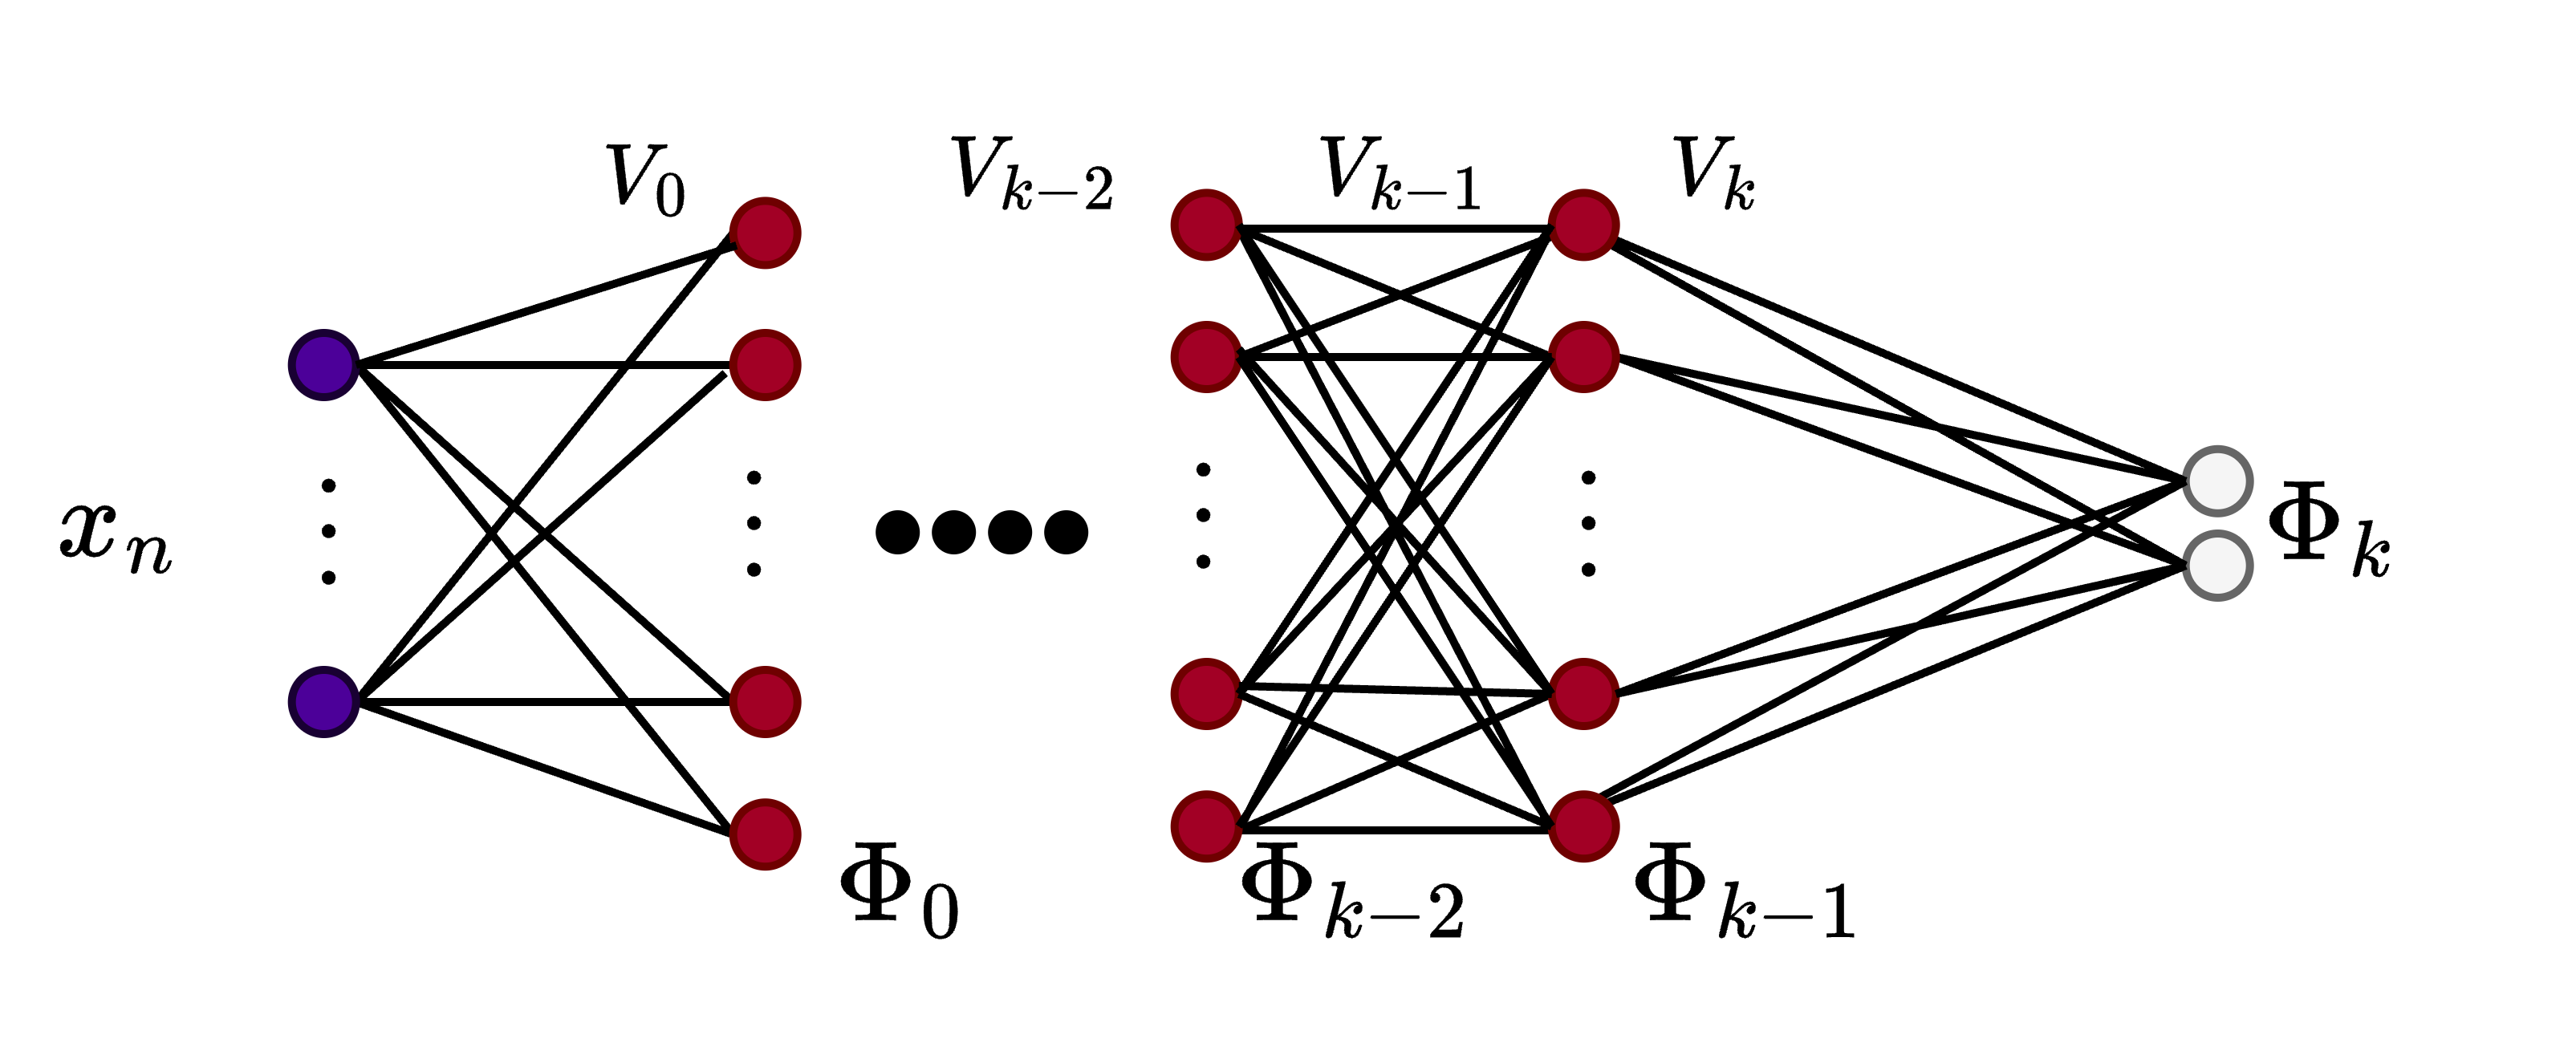
\includegraphics[width=.85\linewidth]{imgs/NN.drawio.png}}
  \caption{Architecture of the deep neural network (DNN).}
  \label{chap2:fig:DNN}
\end{figure}

In general, it was open problem to leverage the DNNs in controllers due to the nonlinearity and mathematically complex architecture of the DNNs.
In \cite{RN13}, Omkar Sudhir Patil \etal proposed the novel DNN based neuro-adaptive control for control-affine nonlinear systems.
The architecture of the DNN in the controller is described in Fig.~\ref{chap2:fig:DNN} and is defined as 
\begin{equation}
  \Phi(x_n;\theta) \triangleq 
  \underbrace{
    V_k^T  \phi_{k}(
    \underbrace{
      V_{k-1}^T   \cdots \phi_2(
      \underbrace
        {
        V_1^T   \phi_1(
        \underbrace
          {
          V_0^T   x_n
        }_{\Phi_0}
        )
      }_{\Phi_1}
      )\cdots )
    }_{\Phi_{k-1}}
    )
  }_{\Phi_k}
  \label{chap2:eq:DNN}
\end{equation}
where $x_n$ denotes the NN input vector, $V_i\in\R^{(l_i+1)\times l_{i+1}}$ is the weight matrix of the $i\textsuperscript{th}$ layer, and $\phi_i: \R^{l_i}\to\R^{l_i+1}$ represents the activation function of the $i\textsuperscript{th}$ layer. 
The element-wise activation function is defined as $\phi_i(x)=[\sigma(x_{(1)}),\sigma(x_{(2)}),\cdots, \sigma(x_{(l_{i})}), 1]^T$, where $\sigma: \R\to\R$ is a nonlinear function, and the augmentation of $1$ is used to account for bias terms in the weight matrices.  
For a better understanding, \eqref{chap2:eq:DNN} also can be represented recursively as 
\begin{equation}
    \Phi_i \triangleq
    \begin{cases}
        V_i^T  \phi_i(\Phi_{i-1}), &i\in[1,\dots,k],\\
        V_0^T  x_n,&i=0,
    \end{cases}
\end{equation}
where $\Phi_i$ denote each layer's output (\ie the last layer's output is equal to the output of DNN such that $\Phi_k = \Phi(x_n;\theta)$).

One of the widely used activation functions for large DNNs is from the ReLU family \cite{RN15}, which effectively avoids the gradient vanishing problem during error backpropagation. 
The gradient vanishing problem occurs when the gradient of the activation function is close to zero, since the gradient of each layer is multiplied using chain rule to backpropagate the error to the inner layers (\ie deeper NNs have high possibility of gradient vanishing).
However, for control applications where relatively shallow DNNs are typically sufficient, and the gradient vanishing issue is less severe, the sigmoid function or the hyperbolic tangent function is commonly used as the activation function. 
These functions simplify stability analysis due to their continuous differentiability, and their outputs and gradients are bounded such that $\Vert \phi_i(\cdot)\Vert < \infty$ and $\Vert \nabla\phi_i(\cdot)\Vert_F < \infty$. 
In this thesis, the hyperbolic tangent function $\tanh(\cdot)$ was selected as the activation function (\ie $\sigma(\cdot) = \tanh(\cdot))$, which provides desirable boundedness with $\Vert\sigma(\cdot)\Vert<1$ and $\Vert\nabla\sigma(\cdot)\Vert< 1$.
Note that, the number of hidden layers should be limited around 5 to avoid the gradient vanishing issue, since the gradient vanishing problem is not addressed.

For simplicity, each layer's weights are vectorized as $\theta_i\triangleq\text{vec}(V_i)\in\R^{\Xi_i}$, where $\Xi_i\triangleq (l_i+1)l_{i+1}$ is the number of weights in the $i\textsuperscript{th}$ layer. 
The total weight vector $\theta\in\R^{\Xi}$ is defined by augmentation $\theta_i$ for all $i\in \left[0,\cdots,k\right]$ as 
\begin{equation}
    \theta \triangleq 
    \begin{bmatrix}
        \theta_k\\
        \theta_{k-1}\\
        \vdots\\
        \theta_0
    \end{bmatrix}
    =
    \begin{bmatrix}
        \text{vec}(V_k)\\
        \text{vec}(V_{k-1})\\
        \vdots\\
        \text{vec}(V_0)
    \end{bmatrix},
\end{equation}
where $\Xi={\sum_{i=0}^{k} \Xi_i}$ represents the total number of weights. 

\subsubsection{Gradient of Deep Neural Network} \label{chap2:sec:DNNgrad}

In the derivation of adaptation law, the gradient of the DNN with respect to the weights is required.
The gradient of $ \Phi(x_n;\theta)$ with respect to $\theta$ is defined as
\begin{equation}
    {\partial\Phi\over\partial \theta}=
    \begin{bmatrix}
        \dfrac{\partial \Phi}{\partial \theta_k}&
        \dfrac{\partial \Phi}{\partial \theta_{k-1}}&
    \cdots &
        \dfrac{\partial \Phi}{\partial \theta_0}
    \end{bmatrix}
    \in\R^{n \times \Xi}
    \label{chap2:eq:DNNgrad}
\end{equation}
where
\begin{equation}
    \frac{\partial \Phi}{\partial \theta_i} = 
    \begin{cases}
        (I_{l_{k+1}}\otimes \phi_{k}^T  ), & i=k \\
        V_k^T   \phi_{k}' (I_{l_{k}}\otimes  \phi_{k-1}^T  ), & i=k-1\\
        &\vdots \\
        V_k^T   \phi'_{k} \cdots V_1^T  \phi_1' (I_{l_1}\otimes x_n^T  ), & i = 0
    \end{cases},
\end{equation}
where $\phi_i\triangleq \phi_i(\Phi_{i-1})$ and $\phi_i'\triangleq \partial \phi_i/\partial \Phi_{i-1}$.
The gradient can be obtained using the chain rule and Proposition \ref{chap2:prop:kron}.


\end{spacing}

%%%%%%%%%%%%%%%%%%%%%%%%%%%%%%%%%%%%
% Chapter 3
%%%%%%%%%%%%%%%%%%%%%%%%%%%%%%%%%%%%

% \begin{spacing}{2.0} % double spacing
\begin{spacing}{1.3} % double spacing
%%%%%%%%%%%%%%%%%%%%%%%%%%%%%%%%
% Chap 3.     CoNAC for Uncertain Euler-Lagrange Systems Under Weight Constraints
%%%%%%%%%%%%%%%%%%%%%%%%%%%%%%%%

\chapter{
    CoNAC for Uncertain Euler-Lagrange Systems Under Weight Constraints
} \label{chapter3}

%%%%%%%%%%%%%%%%%%%%%%%%%%%%%%%%
\section{Introduction} 
%%%%%%%%%%%%%%%%%%%%%%%%%%%%%%%%

In this chapter, a novel constrained optimization based neuro-adaptive control (CoNAC) is presented for uncertain Euler-Lagrange systems with a weight norm constraint. 
As presented in Chapter \ref{chap1:sec:example}, one of the common issues in neuro-adaptive control (NAC) is that the boundedness of neural network’s (NN) weights is not guaranteed.
Since the amplitude of control input of NAC is dependent on the weights, the unbounded weights may lead to instability and severe safety issues. 
The satisfaction of the boundedness of the weights are reformulated into weight norm constraints, which are then incorporated into the CoNAC.

%%%%%%%%%%%%%%%%%%%%%%%%%%%%%%%%
\section{Problem Formulation}
%%%%%%%%%%%%%%%%%%%%%%%%%%%%%%%%

Consider an uncertain Euler-Lagrange system modeled as
\begin{equation}
    M(q)\ddot q + C(q,\dot q)\dot q + G(q) + F(q) = \tau
    \label{chap3:eq:sys1}
\end{equation}
where $q\in \R^n$ and $\tau\in\R^n$ denotes the generalized coordinate and the control input, respectively; $M(q)\in\R^{n\times n}$, $C(q,\dot q)\in\R^{n\times n}$, and $G(q)\in\R^{n}$ denote the unknown system function matrices; and $F(q)\in\R^{n}$ denotes the external force.

Using the user-designed matrices $M_0>0,C_0$ and $G_0$, \eqref{chap3:eq:sys1} can be represented as 
\begin{equation}
    M_0\ddot q+C_0\dot q+G_0 = \tau + f(q,\dot q,\ddot q)
    \label{chap3:eq:sys2}
\end{equation}
where $f(q,\dot q,\ddot q) \triangleq -(M-M_0)\ddot q-(C-C_0)(q,\dot q)\dot q -(G-G_0) -F(q)$ denotes the residual unknown term.

As presented in Section \ref{chap1:sec:example}, the parameter drift (\ie the weights of NNs can diverse) may occur due to the lumped disturbance term.
Hence, the objective of the control design is to make $q$ track the continuously differentiable desired trajectory $q_d(t):\R\to \R^n$ under the unknown terms $f$ while ensuring boundedness of weights of NN in the controller.

%%%%%%%%%%%%%%%%%%%%%%%%%%%%%%%%
\section{Exiting Works for Boundedness of Weights} 
%%%%%%%%%%%%%%%%%%%%%%%%%%%%%%%%

Most studies modify their adaptation laws to ensure the boundedness of the weights.

\subsection{Projection Operator} \label{chap3:sec:proj}

In \cite{RN13, RN11, RN21}, the projection operator is utilized to prevent the weight divergence, by projecting the adaptation direction on some convex set of the weights.
The projection operator is defined in \cite[Appendix E, eq.~(E.4)]{RN7} and represented as
\begin{equation}
    \text{Proj}_\Omega(y)
    =
    \begin{cases}
        \Gamma y
        &
        \begin{aligned}
            &\text{if }x\in\Omega
            \text{ or if }\\
            &x\in\delta\Omega
            \text{ and }
            \nabla c^T\Gamma y\ge0
        \end{aligned}
        \\
        \Gamma y
        -
        \Gamma
        {\nabla c\nabla c^T\over \nabla c^T \Gamma \nabla c}
        \Gamma y
        &
        \text{otherwise}
    \end{cases}
    \label{chap3:eq:proj}
\end{equation}
where $\Gamma=\Gamma^T>0$ is adaptation gain matrix and $y\in\R^n$ denotes the update direction of optimization variable $x\in\R^n$.
Moreover, $\Omega\triangleq \{x\ \vert\ c(x)\le 0\}$ denotes a convex set defined by $c(\cdot)$ is a convex function and $\delta\Omega$ denotes a boundary of $\Omega$.
The convex function $c(\cdot)$ is typically selected as $x^Tx\le \bar x^2$ where $\bar x\in\R_{>0}$ is a maximum norm of $x$.
However, in the literature, the projection operator is only applied to theoretically guarantee the boundedness of the weights, by selecting the convex set as large as possible.
This is because, the authors attempts to estimate the globally ideal weights whose magnitude is unknown.

\subsection{
    \texorpdfstring{$\sigma$}{σ} and \texorpdfstring{$\epsilon$}{ε}-modifications
} 
%  \texorpdfstring{$\mu=0$}{μ=0}

In adaptive control theory, the $\sigma$-modification \cite{RN19} and the $\epsilon$-modification \cite{RN18, RN46} are widely used to regulate the magnitude of the weights by adding a stabilizing function in the adaptation law as follows:
\begin{equation}
    y_\sigma = \Gamma (y+\lambda x)
    ,
    \quad
    y_\epsilon = \Gamma (y+\rho\Vert e\Vert x)
\end{equation}
where $y_i,\ i\in[\sigma,\epsilon]$ denote adaptation laws of $\sigma$-modification and $\epsilon$-modification, respectively, $e$ denotes tracking error, and $\lambda$ and $\rho$ denote parameters of $\sigma$-modification and $\epsilon$-modification, respectively.
These methods make the invariance set of the estimation error of the weights over time.
The existing methods have shown their effectiveness in ensuring the boundedness of the weights via numerical simulations.
However, the weights are biased to the origin by the stabilizing function, which may degrade the performance of the controller.
This means that there is a trade-off between the boundedness of the weights and the optimality of the weights.
Moreover, they lack theoretical analysis regarding the optimality of the adapted weights.

Interestingly, similar approaches that regulate the magnitude of the weights have also been introduced in the deep learning literature.
One of the approaches is $L_2$-regularization, which adds the squared magnitudes of the weights to the objective function \cite{RN34, RN36}.
Then, the adaptation process attempts to reduce not only the original objective function, but also the magnitude of the weights.
By regulating the magnitude of the weights, the stability of the adaptation process can be enhanced, and overfitting can be prevented.
However, $L_2$-regularization also involves same limitations as $\sigma$ and $\epsilon$-modifications.

%%%%%%%%%%%%%%%%%%%%%%%%%%%%%%%%
\section{CoNAC with Weight Norm Constraint} \label{chap3:problem} 
%%%%%%%%%%%%%%%%%%%%%%%%%%%%%%%%

Without loss of generality a single hidden layer neural network (SHLNN) is utilized in this chapter for better intuition and simplicity. 
Note that SHLNN is the simplest case of DNN presented in Section \ref{chap2:sec:DNN}.
The architecture of the CoNAC is illustrated in Fig.~\ref{chap3:fig:ctrl}, consisting of: a reference generator, the SHLNN that functions as NAC, and a weight optimizer for the SHLNN. 
The reference generator is designed based on backstepping control (BSC), presented in previous Section \ref{chap2:sec:ctrl} , to generate a tracking reference for both $q$ and $\dot q$.

\begin{figure*}[t]
    \centering
    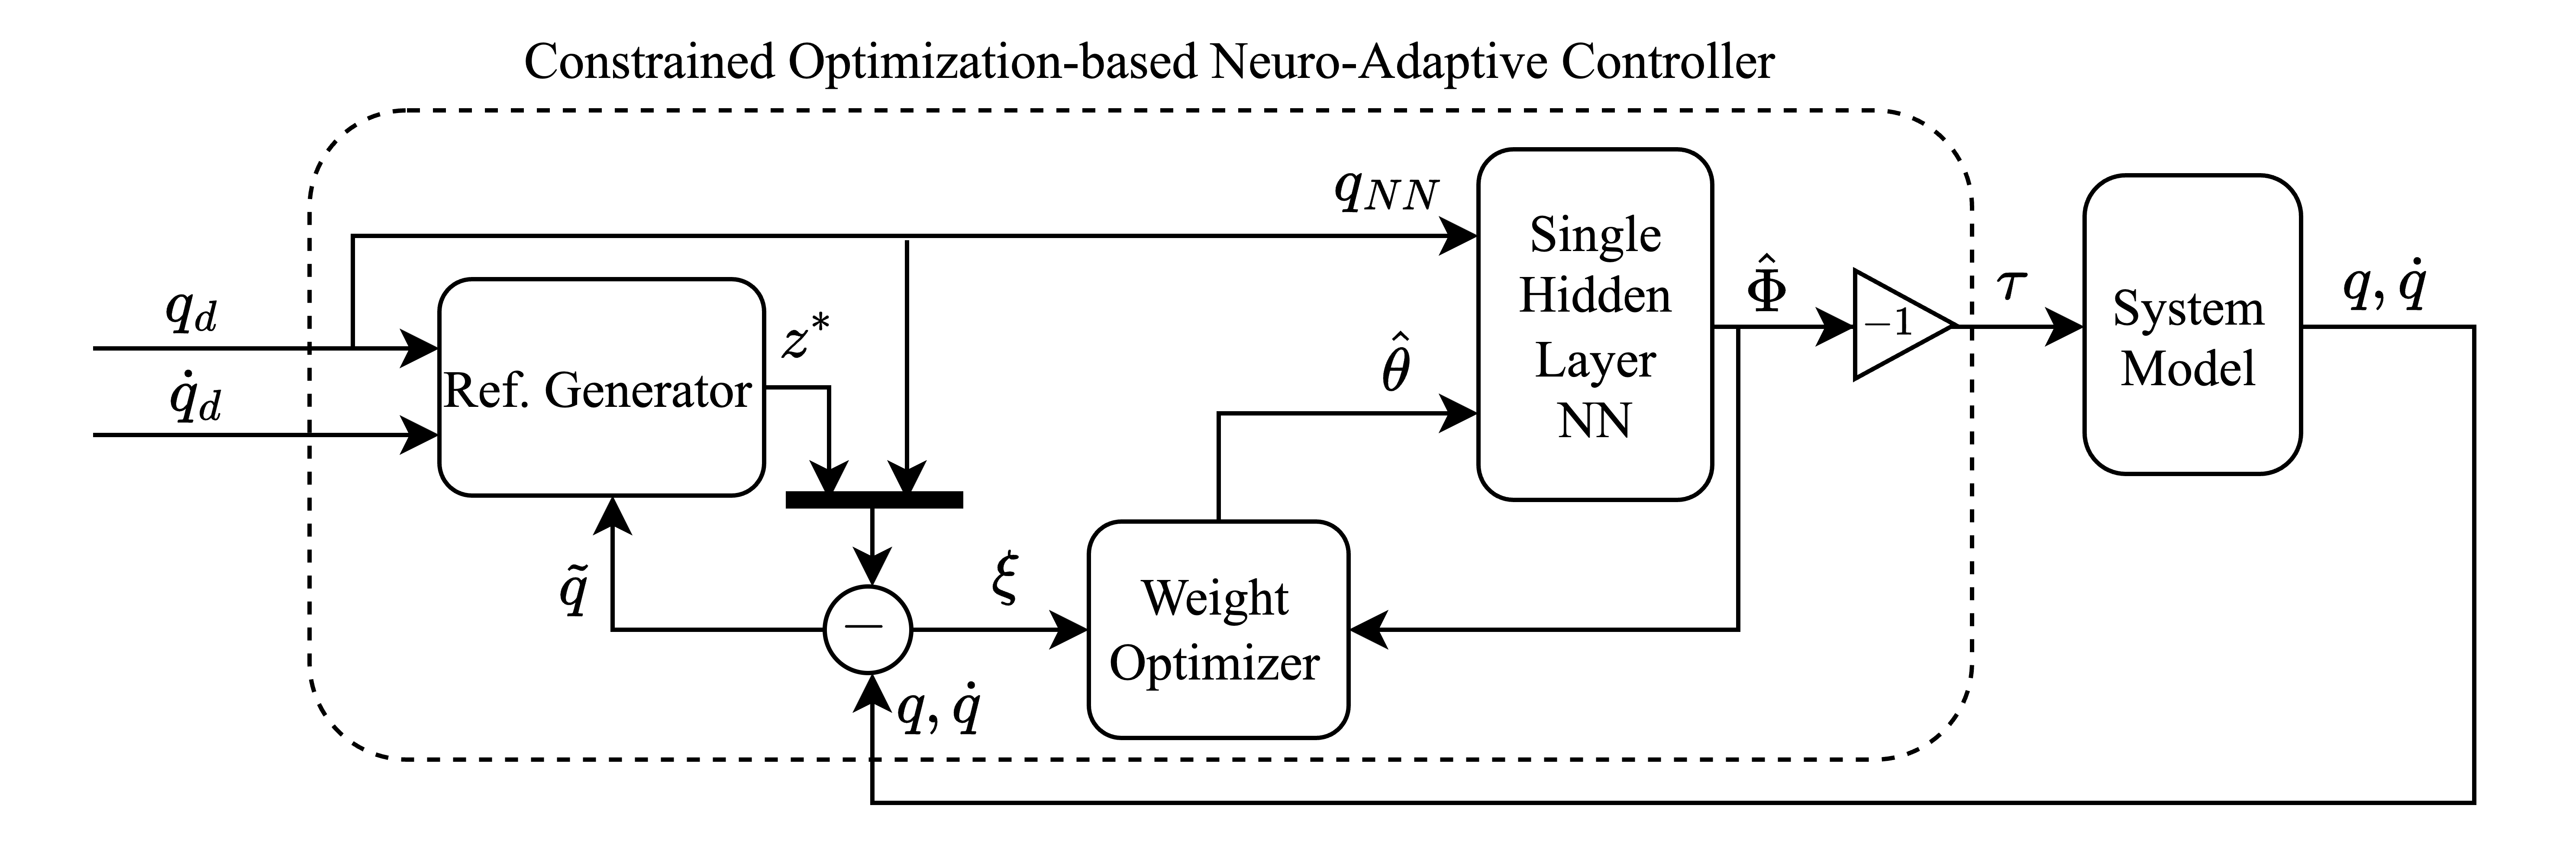
\includegraphics[width=0.9\linewidth]{imgs/ControllerChap3.drawio.png}
    \caption{Architecture of the constrained optimization-based neuro-adaptive controller (CoNAC).}
    \label{chap3:fig:ctrl}
\end{figure*}

\subsection{Control Law Development} \label{chap3:sec:ctrl_dev}

The system dynamics \eqref{chap3:eq:sys2} can be represented as
\begin{equation}
    \begin{aligned}
        \dot {q} &= {z},\\
        \dot {z} &= -M_0^{-1} C_0 {z}-M_0^{-1} G_0+M_0^{-1} h(\tau) + M_0^{-1} f,
    \end{aligned}
    \label{chap3:eq:x_dyna}
\end{equation}
where ${z}\triangleq \dot q$.

Consider the Lyapunov function ${\mathcal V}_{c1}\triangleq(1/2){\tilde q}^T  {\tilde q}$, where ${\tilde q}\triangleq {q}-{q_d}$ represents the tracking error between the actual trajectory ${q}$ and the desired trajectory $q_d$. 
The desired trajectory of ${z}$, ensuring $\dot {\mathcal V}_{c1}={\tilde q}^T  ({z}-\dot {q_d})<0$ is 
\begin{equation}
    {z^*} \triangleq -{k_q}{\tilde q} + \dot q_d,
\end{equation}
which functions as the reference generator with control gain ${k_q} \in\R_{>0}$. The tracking error of ${z}$ relative to the desired trajectory ${z^*}$ is defined as
\begin{equation}
    {\tilde z} \triangleq {z} - {z^*} = {z} - (-{k_q}{\tilde q} + \dot q_d).
    \label{chap3:eq:e2}
\end{equation}

Next, consider the Lyapunov function ${\mathcal V}_{c2}\triangleq {\mathcal V}_{c1} + (1/2) {\tilde z}^T  {\tilde z}$.
Its time derivative is
\begin{equation}
    \begin{aligned}
    \dot {\mathcal V}_{c2} &=
    {\tilde q}^T  (-{k_q}{\tilde q}+{\tilde z}) +{\tilde z}^T  (-M_0^{-1} C _0{z} -M_0^{-1} G_0\\
    &\quad
    +M_0^{-1}h(\tau)+M_0^{-1} f- \dot z^*)\\
    &= -{k_q}{\tilde q}^T  {\tilde q} -{k_z}{\tilde z}^T  {\tilde z} +{\tilde z}^T  ({k_z}{\tilde z}+{\tilde q}\\
    &\quad-M_0^{-1} C_0{z} -M_0^{-1} G_0+M_0^{-1} h(\tau)+M_0^{-1} f- \dot z^* )
    \end{aligned}
\end{equation}
with control gain ${k_z}\in\R_{>0}$. 
The stabilizing control law, which does not account for weight norm and input constraints, is defined as follows:
\begin{equation}
    \tau^* \triangleq-M_0\cdot ({k_z}{\tilde z})+ 
    ( 
        -M_0{\tilde q}+C_0{z}+G_0-f+M_0 \dot z^*
    )
    .
    \label{chap3:eq:desired_control}
\end{equation}
This control law ensures that the time derivative of the Lyapunov function is negative definite, as $\dot {\mathcal V}_{c2} = -{k_q}{\tilde q}^T  {\tilde q}-{k_z}{\tilde z}^T  {\tilde z}<0$, in the absence of any constraints. 
However, the control law $\tau^*$ cannot be realized in practice because the lumped system uncertainty function $f$, which accounts for unmodeled dynamics and disturbances, is not available.

As introduced in Section \ref{chap2:sec:DNN}, the SHLNN which is simple version of DNN is represented as 
\begin{equation}
    \Phi({q_{NN}};\theta)\triangleq V_1^T\phi(V_0^T{q_{NN}})
\end{equation}
where ${q_{NN}}\in\R^{l_0+1}$ denotes the NN input vector, $V_i\in\R^{(l_i+1)\times l_{i+1}},\ i\in[0,1]$ denotes the weight matrix of $i\textsuperscript{th}$ layer and $\phi:\R^{l_1}\to\R^{l_1+1}$ denotes the activation function layer.
The element-wise activation function layer consists of nonlinear function $\sigma(\cdot)$ and augmented $1$ to combine the bias term in weight matrix (\ie $\phi(x) = [\sigma(x_{(1)}),\cdots, \sigma(x_{(l_1)}), 1]^T$).
For further simplicity, let $\theta\triangleq[\theta_1^T,\theta_0^T]^T\in\R^{\Xi}$ denote the total weight vector, where $\theta_i\triangleq \text{vec}(V_i)\in\R^{\Xi_i}$ denote the vectorized weights.
$\Xi_i=(l_i+1)\cdot l_{i+1}$ and $\Xi=\Xi_0+\Xi_1$ denote the number of each layer and total weights, respectively.

Using this SHLNN, the desired controller $\tau^*$ can be approximated through ideal weight vector $\theta^*$ for a compact subset $\Omega_{NN}\in\R^{l_0+1}$ to $\epsilon$-accuracy according to Theorem \ref{chap2:thm:uni_approx} such that $\sup_{{q_{NN}}\in\Omega_{NN}} \Vert\Phi({q_{NN}};\theta^*) - \tau^*\Vert=\epsilon<\infty$.
The ideal weight vector $\theta^*$ is typically assumed to be bounded.
In this thesis, $\theta^*$ is defined as a local optimal point, rather than a global optimal point.
Then using the estimated weight vector $\hat\theta=[\hat\theta_1^T,\hat\theta_0^T]^T$ of $\theta^*=[\theta_1^{*T},\theta_0^{*T}]^T$, the desired controller $\tau^*\approx -\Phi(q_{NN};\theta^*)-\epsilon$ can be approximated as follows:
\begin{equation}
    \tau \triangleq -\Phi({q_{NN}};\hat\theta)
    .
    \label{chap3:eq:approx_control}
\end{equation}
For further sections, let $\Phi^*\triangleq\Phi({q_{NN}};\theta^*)$ and $\phi^* \triangleq\phi(V_0^{*T}{q_{NN}})$, and $\hat\Phi\triangleq\Phi({q_{NN}};\hat\theta)$, $\hat\phi \triangleq\phi(\hat V_0^{T}{q_{NN}})$ and $\hat\phi' = \partial \hat\phi/\partial (\hat V_0^Tq_{NN})$.

Using \eqref{chap3:eq:x_dyna}, \eqref{chap3:eq:e2}, \eqref{chap3:eq:desired_control}, and \eqref{chap3:eq:approx_control}, the error dynamics can be derived as
\begin{equation}
    \begin{aligned}
        \dot {\tilde q} = & -{k_q} {\tilde q} + {\tilde z} \\
        \dot {\tilde z} = & -{\tilde q} -{k_z} {\tilde z} + M_0^{-1} (\Phi^*-\hat\Phi+\epsilon).
    \end{aligned}
    \label{chap3:eq:e_dyna}
\end{equation}
The error dynamics \eqref{chap3:eq:e_dyna} can be represented as a first-order system: 
\begin{equation}
    \dot\xi = A_\xi \xi + B_\xi (\Phi^*-\hat\Phi+\epsilon)
    \label{chap3:eq:xi_dyna}
\end{equation}
where $\xi\triangleq[{\tilde q}^T  , {\tilde z}^T  ]^T  \in\R^{2n}$ denotes the augmented error, and
\begin{equation}
    A_\xi \triangleq 
    \begin{bmatrix}
        -{k_q} I_n &I_n\\-I_n& -{k_z} I_n
    \end{bmatrix}
    ,\ 
    B_\xi \triangleq 
    \begin{bmatrix}
        0_{n\times n}\\M_0^{-1}
    \end{bmatrix}
    .
\end{equation}
Note that $A_\xi$ is a stable matrix, and $\Vert B_\xi\Vert_F<\infty$.

\subsection{Weight Adaptation Laws} \label{chap3:sec:weight_adap}

% \subsection{Adaptation Law using Lagrangian Function}
\subsubsection{Weight Optimizer Design}

Consider a positive definite objective function defined as 
\begin{equation}
    J(\xi;\hat\theta)\triangleq 
    {1\over 2} \xi^T   W\xi
\end{equation}
where $W=W^T  >0$ is a weighting matrix.
The weight norm constraints $c_j,\ j\in\mathcal{I}$ presented in following Section \ref{chap3:sec:weight_cstr}, are imposed during the weight adaptation process, where $\mathcal I$ denotes the set of the imposed inequality constraints.
The corresponding constrained optimization problem is formulated as
\begin{equation}
    \underset{\hat\theta}{\text{minimize}}\quad J(\xi;\hat\theta),
    \quad\quad
    \text{subject to }
    c_{j}(\hat\theta)\le0, \  \forall j\in\mathcal{I}
    . 
    \label{chap3:eq:train_obj}
\end{equation}
% where $q_a$ is an additional vector in the constraints.
Here, tracking error $\xi$ is considered a pre-defined data or parameter for this optimization problem. The Lagrangian function is defined as
\begin{equation}
    L(\xi,\hat\theta,[\lambda_j]_{j\in\mathcal A}) \triangleq J(\xi;\hat\theta) + 
    \sum_{j\in\mathcal A}
    \lambda_{j}
    c_{j}(\hat\theta)
\end{equation}
where $\lambda_j$ denotes the Lagrange multiplier for each constraint, and $\mathcal A \triangleq \{j\in\mathcal I\ |\ c_j\ge 0\}$ represents the active set.

The adaptation laws for $\hat\theta$ and $[\lambda]_{j\in\mathcal A}$ are derived to solve the dual problem of \eqref{chap3:eq:train_obj} (\ie  $\min_{\hat\theta} \max_{[\lambda]_{j\in\mathcal A}}L(\xi,\hat\theta,[\lambda]_{j\in\mathcal A})$), as follows:
\begin{subequations}
    % \begin{equation}
    \begin{align}
            \dot {\hat\theta}&=-\alpha {\partial L\over\partial \hat\theta}
            =-\alpha 
            \bigg(
            {\partial J\over \partial \hat\theta}+\sum_{j\in\mathcal{A}}
            \lambda_j {\partial c_j\over\partial \hat\theta}
            \bigg),
        \label{chap3:eq:adap_th}
            \\
            \dot\lambda_j& = \beta_j{\partial L\over\partial \lambda_j} = \beta_j c_j ,
            \quad\quad\quad\quad      \      
            \forall j\in\mathcal A,
        \label{chap3:eq:adap_L}
            \\
            \lambda_j & = \max(\lambda_j,0) ,
            \quad\quad\quad\quad\ \ \ \ \ 
            \forall j\in\mathcal A,
        \label{chap3:eq:adap_L_max}
    \end{align}
    \label{chap3:eq:adap}
    % \end{equation}
\end{subequations}
where $\alpha\in\R_{>0}$ denotes the adaptation gain (also known as learning rate) and $\beta_j\in\R_{>0}$ denotes the update rate of the Lagrange multipliers in $\mathcal A$. 
The Lagrange multipliers associated with inequality constraints are non-negative.
When a constraint $c_j$ becomes active (\ie violated), the corresponding Lagrange multiplier $\lambda_j$ increases from zero to address the violation by adjusting the weights' adaptation direction $\dot{\hat\theta}$. 
Once the violation is resolved and the constraint is no longer active (\ie $c_j < 0$), the multiplier decreases gradually until it returns to zero. 
Note that this adaption law is similar to the augmented Lagrangian method (ALM) in \cite{RN22}, where the adaptation law for Lagrange multipliers is given by $\lambda_j\leftarrow \text{max}(\lambda_j-c_j/\mu,0)$, with $\mu\in\R_{>0}$ being the penalty parameter. 
    
At steady state, where $\dot{\hat\theta}=0$ and $\dot\lambda_j=0$, the KKT conditions defined in Theorem \ref{chap2:thm:KKT}, are satisfied, \ie $\partial L/\partial \hat\theta=0$, $c_j \le 0$, $\lambda_j \ge 0$, and $\lambda_j c_j=0$.
In other words, the proposed optimizer updates the SHLNN weights and Lagrange multipliers in a way that satisfies the KKT conditions. 
These conditions represent the first-order necessary conditions for optimality, guiding the updates toward candidates for a locally optimal point.

\subsubsection{Calculation of the Exact Gradient of Objective Function}

The adaptation law for $\hat\theta$ involves the gradient of the objective function with respect to $\hat\theta$ (\ie ${\partial J/\partial \hat\theta}$); see \eqref{chap3:eq:adap_th}. Since the objective function depends on the state $\xi$ of a dynamic system, obtaining the gradient is not straightforward. Therefore, the forward sensitivity method from \cite{RN49} is employed to calculate the exact gradient of the objective function. 

By partially differentiating \eqref{chap3:eq:xi_dyna}, the sensitivity equation of $\xi$ with respect to $\hat\theta$ is first obtained as
\begin{equation}
    \dot\eta = A_\xi\eta - B_\xi{\partial\hat\Phi\over\partial\hat\theta}
    \label{chap3:eq:eta_dyna}
\end{equation}
where $\eta \triangleq \partial \xi/\partial \hat\theta\in\R^{2n\times \Xi}$.
Since the initial value of $\xi$ is independent to $\hat\theta$, $\eta\vert_{t=0}$ is a zero matrix. 
The gradient of the objective function with respect to $\hat\theta$ is then obtained as 
\begin{equation}
   {\partial J\over\partial \hat\theta} =  {\partial \xi\over \partial \hat\theta}^T  W\xi=\eta^T  W\xi\in\R^\Xi.
   \label{chap3:eq:dJdth}
\end{equation}
Equations \eqref{chap3:eq:eta_dyna} and \eqref{chap3:eq:dJdth} can be decomposed for each layer as 
\begin{equation}
  \begin{aligned}
    \dot\eta =&
    \begin{bmatrix}
        \eta_1&\eta_0
    \end{bmatrix}'
    \\
    =&A_\xi
    \begin{bmatrix}
        \eta_1&\eta_0
    \end{bmatrix}
    -B_\xi
    \begin{bmatrix}
        (I_{l_2}\otimes \hat\phi^T)&\hat V_1^T\hat\phi'(I_{l_1}\otimes {q_{NN}}^T)
    \end{bmatrix}
    .
  \end{aligned}
  \label{chap3:eq:eta_dyna_decomp}
\end{equation}
and
\begin{equation}
    {\partial J\over\partial\hat\theta}
    =
    \begin{bmatrix}
        \partial J/\partial\hat\theta_1\\\partial J/\partial\hat\theta_0\\
    \end{bmatrix}    =
    \begin{bmatrix}
        \eta_1^T\\\eta_0^T\\
    \end{bmatrix}
    W
    \xi
\end{equation}
where $\eta_i \triangleq \partial \xi/\partial \hat\theta_i\in\R^{2n\times \Xi_i}$. 
The exact gradient of the objective function is calculated based on \eqref{chap3:eq:dJdth}, with the value of $\eta$ obtained by simulating the sensitivity equation \eqref{chap3:eq:eta_dyna}.

The proposed controller is implemented using Algorithm \ref{chap3:alg:alg1}. 
For implementation in the discrete-time domain, it is recommended to use a sufficiently small sampling time $T_s$. 
If a large $T_s$ is used, $\alpha$ and $\beta_j$ should satisfy the Armijo condition \cite[Chap.~3 eq.~(3.4)]{RN9} to ensure that the objective function decreases.

\begin{algorithm}[t]
    \caption{Weight optimizer implementation.}\label{chap3:alg:alg1}
    \SetKwInOut{Input}{input}
    \SetKwInOut{Output}{output}
        \Input{$\xi$, $\hat\theta$, $\lambda_j$, $\eta$}
        \Output{$\hat\theta$, $\lambda_j$, $\eta$}
        \BlankLine
        \emph{Set $\mathcal A \leftarrow \mathcal A\cup \{j\}$ for all $c_j\ge0$}\;
        \emph{Determine update matrix $\dot\eta$ using \eqref{chap3:eq:eta_dyna}}\;
        \emph{Update $\eta\leftarrow \eta +\dot\eta\cdot T_s$}\; 
        \emph{Determine update directions $\dot{\hat\theta}$, $[\dot\lambda_j]_{j\in\mathcal A}$ using \eqref{chap3:eq:adap_th}, \eqref{chap3:eq:adap_L}}\;
        \emph{Update weight vector $\hat\theta\leftarrow \hat\theta+\dot{\hat\theta}\cdot T_s$}\;
        \emph{Update multipliers $[\lambda_j]_{j\in\mathcal A}\leftarrow [\lambda_j]_{j\in\mathcal A}+[\dot\lambda_j]_{j\in\mathcal A}\cdot T_s$}\;
        \emph{$[\lambda_j]_{j\in\mathcal A}\leftarrow \max([\lambda_j]_{j\in\mathcal A}, 0)$}\;
        \emph{Set $\mathcal A \leftarrow \mathcal A - \{j\}$ for all $\lambda_j=0$}\;
\end{algorithm}

%%%%%%%%%%%%%%%%%%%%%%%%%%%%%%%%
\section{Weight Norm Constraint} \label{chap3:sec:weight_cstr}
%%%%%%%%%%%%%%%%%%%%%%%%%%%%%%%%

\begin{figure*}[t]
  \centering
  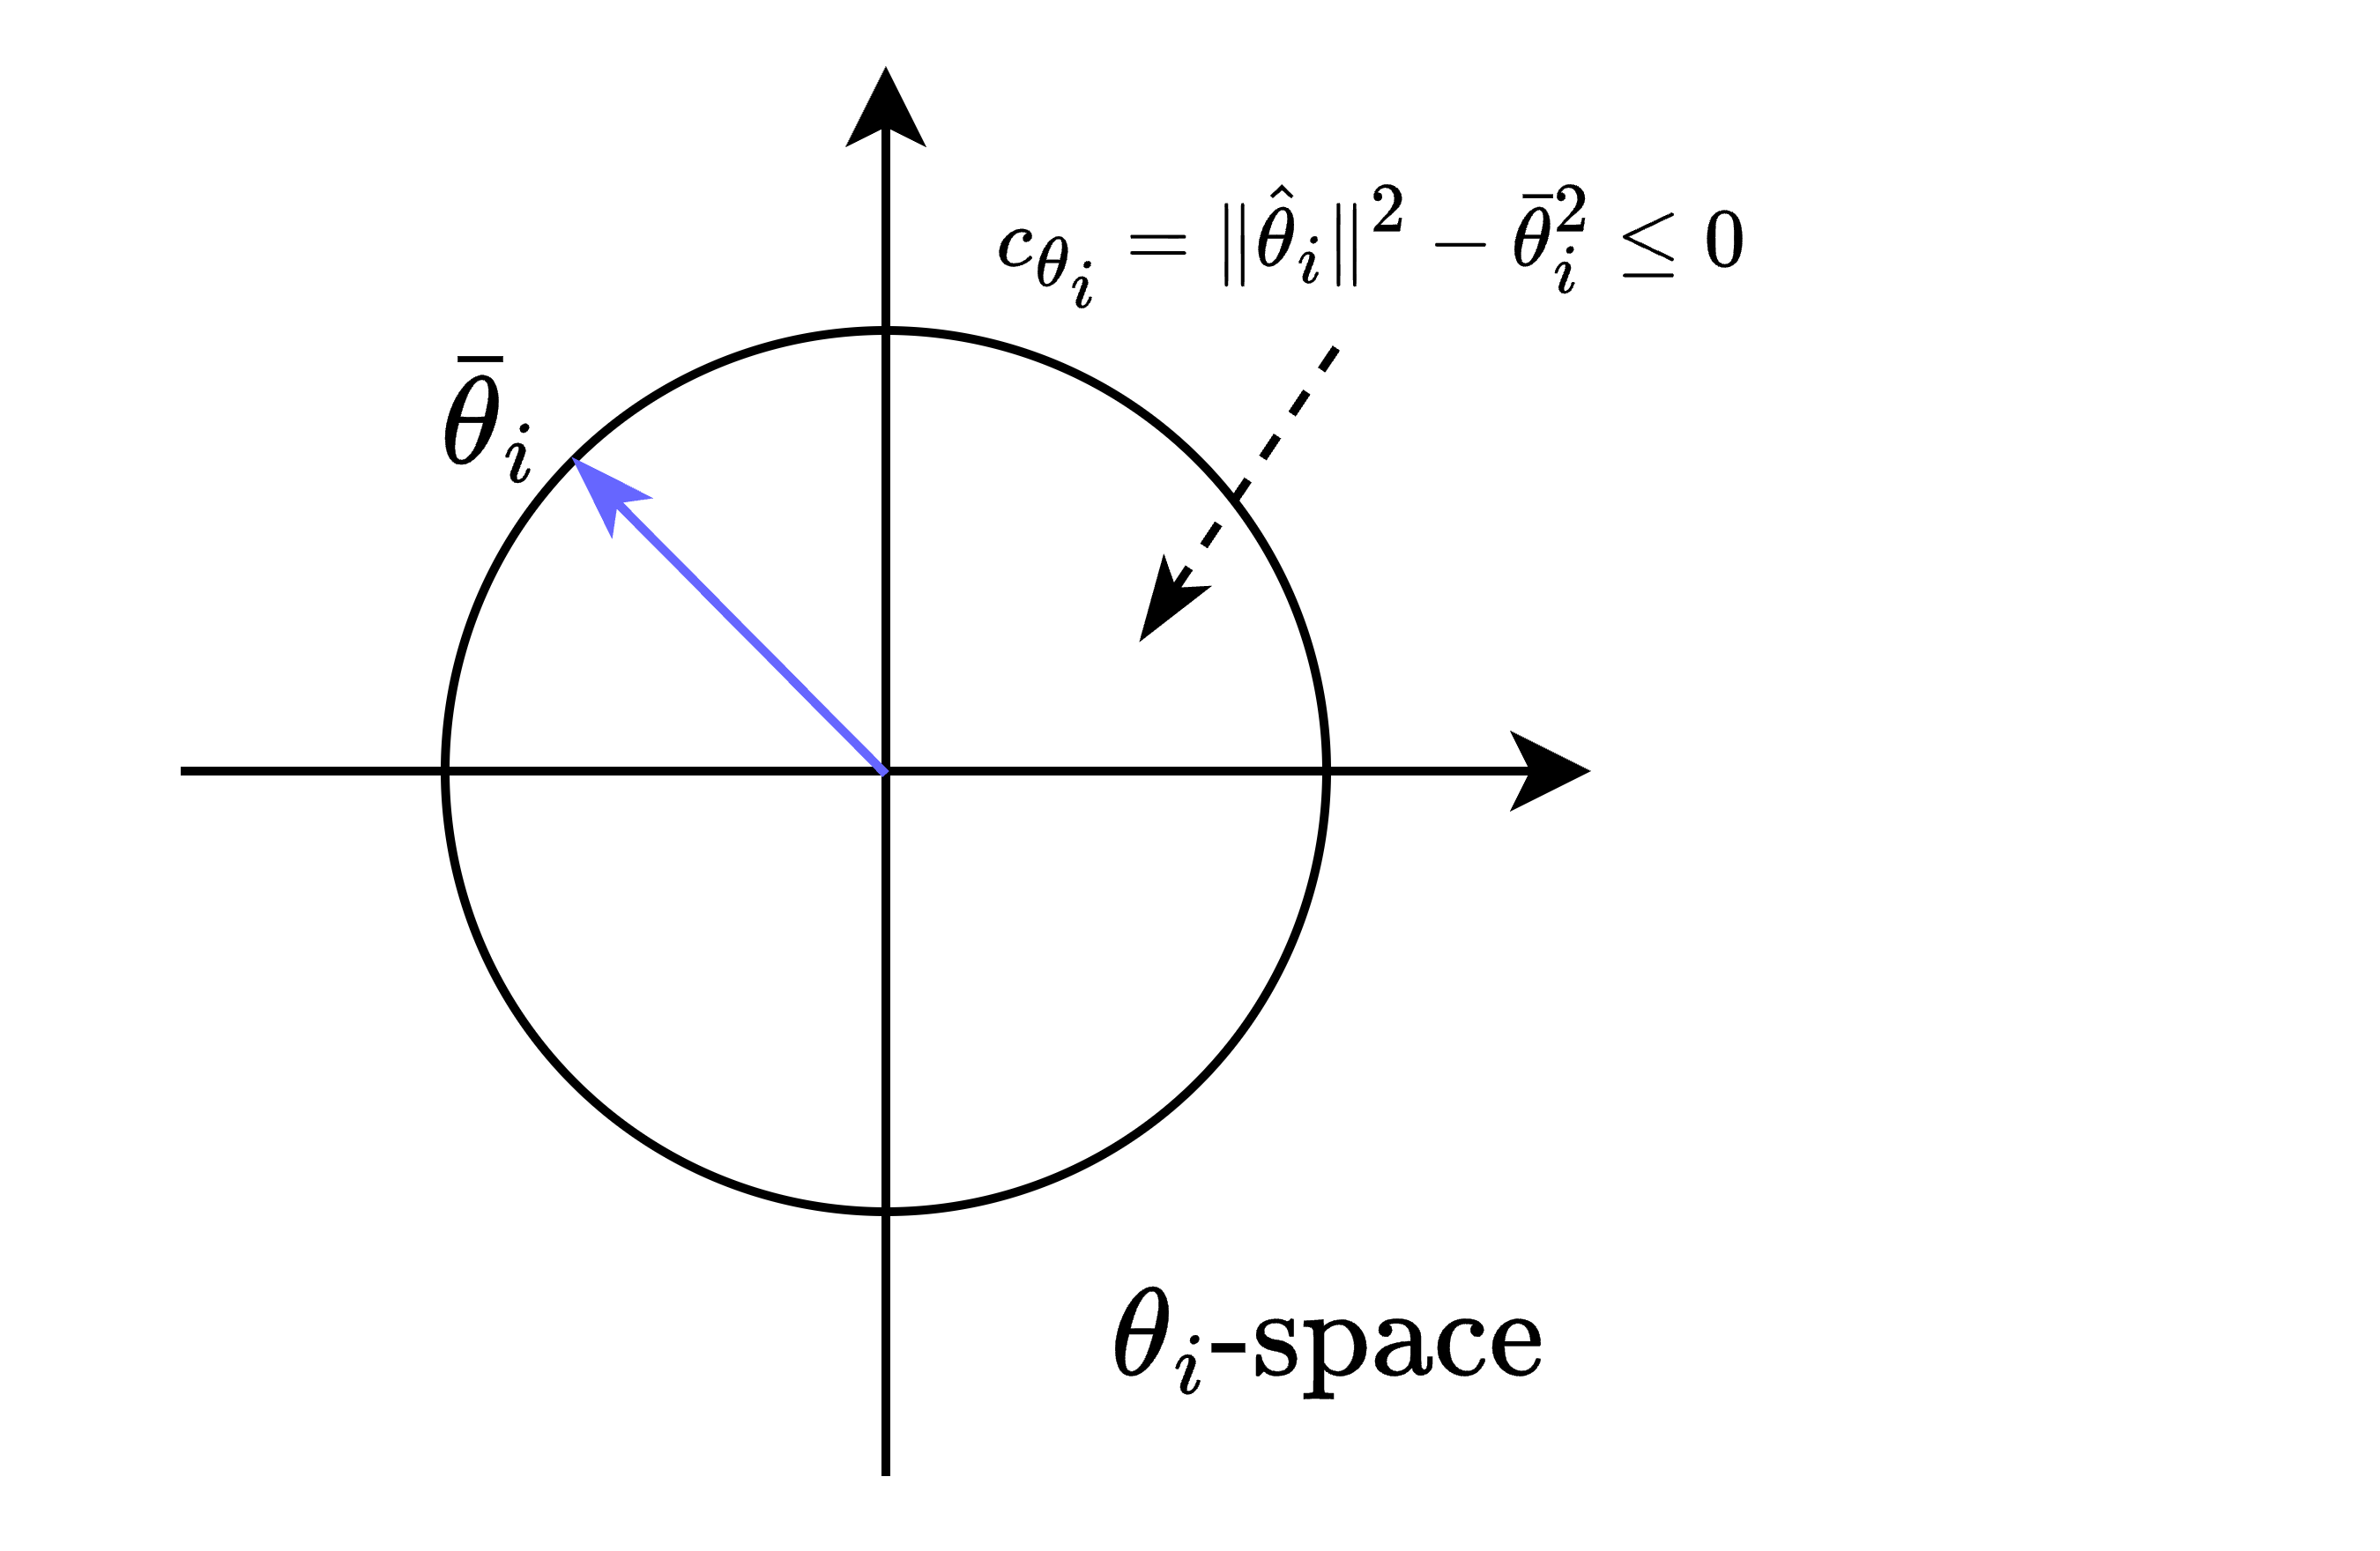
\includegraphics[width=0.5\linewidth]{imgs/cstr_weight.drawio.png}
  \caption{Weight norm constraints.}
  \label{chap3:fig:cstr:weight}
\end{figure*}

The satisfaction of the weights' boundedness is reformulated as a weight norm constraints as shown in Fig.~\ref{chap3:fig:cstr:weight}.
The weight norm constraints are represented as follows:
\begin{equation}
    \begin{aligned}
        c_{\theta_1}(\hat\theta) &\triangleq \Vert \hat\theta_1\Vert^2 - \bar\theta_1^2 \le 0,\\
        c_{\theta_0}(\hat\theta) &\triangleq \Vert \hat\theta_0\Vert^2 - \bar\theta_0^2 \le 0,
    \end{aligned}
    \label{chap3:eq:cstr:weight}
\end{equation}
where $\bar\theta_i^2\in\R_{>0}$ denotes the predefined weight norm bound for each layer $i\in[0,1]$.

The gradient of the constraints can be obtained easily as follows:
\begin{equation}
  \frac{\partial c_{\theta_0}}{\partial\hat\theta}
  = 
  \begin{bmatrix}
      0_{\Xi_1\times 1} \\
      2\hat\theta_0 
  \end{bmatrix}
  ,\quad
  \frac{\partial c_{\theta_1}}{\partial\hat\theta}    
  = 
  \begin{bmatrix}
      2\hat\theta_1 \\
      0_{\Xi_0\times 1}
  \end{bmatrix}
  .
  \label{chap3:eq:cstr:weight_grad}
\end{equation}

%%%%%%%%%%%%%%%%%%%%%%%%%%%%%%%%
\section{Stability Analysis}
%%%%%%%%%%%%%%%%%%%%%%%%%%%%%%%%

The following theorem proves the boundedness of the tracking error and the weight estimation of the weights.

\begin{theorem}
    For the dynamical system in \eqref{chap3:eq:sys1}, the proposed controller \eqref{chap3:eq:approx_control} and the adaptation law \eqref{chap3:eq:adap} ensure the boundedness of the tracking error $\xi$ and the weight estimation $\hat\theta$, provided that control gains ${k_q}$ and ${k_z}$ satisfy \eqref{chap3:eq:stable_cond}.
\end{theorem}

\begin{proof}

The boundedness will be proved from the last layer to the first layer.

\subsubsection{Step 1: Boundedness of $\hat\theta_1,\eta_1,\xi$}

For convenience, assume that all constraints are in the active set without loss of generality.
If the constraints are not in the active set, the boundedness cannot be guaranteed, but weights will be adapted to reduce the objective function until the constraints are violated.

The dynamics of $\xi$ can be represented as
\begin{equation}    
    \dot \xi = A_\xi\xi +B_\xi
    (
        -\hat V_1^T \hat\phi+w(t)
    )
\end{equation}
where $w(t)\triangleq V_1^{*T}\phi^*+\epsilon$ is a lumped residual term, which is bounded as $\Vert w(t)\Vert\le \bar w< 0$.
On the other hand, the dynamics of $\eta_1$ and $\hat\theta_1$ are represented as
\begin{equation}
    \begin{aligned}
        \dot\eta_1 =
        & 
        A_\xi \eta_1 -B_\xi (I_{l_{2}}\otimes \hat\phi^T)
        \\
        \dot{\hat\theta}_1 =
        & -\alpha 
        (
            \eta_1^TW\xi+2\lambda_{\theta_1} \hat\theta_1
        ).
    \end{aligned} 
\end{equation}
According to Theorem \ref{chap2:thm:BIBO}, the boundedness of $\eta_1$ can be obtained, since $A_\xi$ is stable and the residual term $-B_\xi (I_{l_{2}}\otimes \hat\phi^T)$ is bounded.

Define the Lyapunov function $\mathcal V_1=(1/2)\xi^TP\xi+(1/2\alpha)\tilde\theta_1^T\tilde\theta_1$, with the Lyapunov equation $A_\xi^TP+PA_\xi=-Q$, where $A_\xi<0,P=P^T>0$, and $Q>0$.
Using Proposition \ref{chap2:prop:kron} (\ie $\hat V_1^T\hat\phi = \text{vec}(\hat V_1^T\hat\phi)=\text{vec}(\hat\phi^T\hat V_1) = (I_{l_2}\otimes \hat\theta^T)\text{vec}(\hat V_1)=(I_{l_2}\otimes \hat\phi^T)\hat\theta_1$), the time derivative of $\mathcal V_1$ is
\begin{equation}
    \begin{aligned}
        \dot {\mathcal V}_1 =& {1\over 2}\xi^T(A_\xi^TP+PA_\xi)\xi+\xi ^TP ( -B_\xi\hat V_1^T\hat \phi   +B_\xi w(t) )+\hat\theta_1^T
        \bigg(
            -\eta_1^TW \xi-2\lambda_{\theta_1} \hat\theta_1 
        \bigg)
        \\
        =& -{1\over 2}\xi^TQ\xi -\xi^TPB_\xi(I_{l_2}\otimes \hat\phi^T)\hat\theta_1 +\xi^T\Delta
        -\hat\theta_1^T\eta_1^TW\xi
        -2\lambda_{\theta_1} \hat\theta_1^T\hat\theta_1
        \\
        \le& -(1/2)\lambda_\text{min}(Q)\Vert \xi\Vert ^2
        +\bar\Delta \Vert \xi\Vert  
        +\bar M\Vert \xi\Vert  \Vert \hat\theta_1\Vert
        -2\lambda_{\theta_1}
        \Vert\hat\theta_1\Vert ^2
        \\
        \le& 
        \bigg(
        -{\lambda_\text{min}(Q)\over 2} +{\bar M\over 2}
        \bigg)
        \Vert \xi\Vert ^2 +\bar\Delta \Vert \xi\Vert  
        + 
        \bigg(
        -2\lambda_{\theta_1} 
        +{\bar M\over 2}
        \bigg)
        \Vert \tilde\theta_1\Vert ^2 
        \end{aligned}
        \label{chap3:eq:V1_dot}
\end{equation}
where $\Delta\triangleq PB_\xi w(t)$ and $M\triangleq  -PB_\xi(I_{l_2}\otimes \hat\phi^T)+W\eta_1$ which are bounded such that $\Vert\Delta\Vert\le\bar\Delta<\infty$ and $\Vert M\Vert_F\le \bar M< \infty$, respectively.

By defining $P=I_n$, the eigenvalues of $Q=-A_\xi^T-A_\xi$ are $2k_q$ and $2k_z$, since $A_\xi$ is a skew-symmetric matrix except for the diagonal entries.
According to \eqref{chap3:eq:V1_dot}, if $k_q$ and $k_z$ are provided that
\begin{equation}
    \text{min}(k_q,k_z)>\bar M/2
    ,
    \label{chap3:eq:stable_cond}
\end{equation}
and if $\lambda_{\theta_1}$ is increased sufficiently large such that $2\lambda_{\theta_1}>\bar M/2$, due to the violation of the $c_{\theta_1}$, the tracking error is bounded in 
\begin{equation}
    \Theta_\xi = 
    \bigg\{
        \xi \ \bigg\vert\ \Vert\xi\Vert \le  
        {
            \bar \Delta \over \lambda _\text{min}(Q)-\bar M/2
        } 
    \bigg\}
    ,
\end{equation}
and the weight estimation $\theta^*_1$ is bounded in 
\begin{equation}
    \Theta_{\hat\theta_1} = 
    \{ 
        \hat\theta 
        \ 
        \vert
        \ 
        \Vert\hat\theta\Vert \le  
        \bar\theta_1
    \}
    .
\end{equation}
The Lagrange multiplier $\lambda_{\theta_1}$ is also bounded, since $\lambda_{\theta_1}$ update halts once $\hat\theta_1$ approaches into the compact set $\Theta_{\hat\theta_1}$, satisfying the constraint $c_{\theta_1}$.

\subsubsection{Step 2: Boundedness of $\hat\theta_0,\eta_0$}

The dynamics of $\eta_0$ and $\hat\theta_0$ are represented as
\begin{equation}
    \begin{aligned}     
        \dot\eta_0 =& 
        A_\xi\eta_0 -B_\xi 
        \hat V_1^T\hat\phi'(I_1\otimes {q_{NN}}^T)
        \\
        \dot{\hat\theta}_0
        =&
        -\alpha 
        \bigg(
            \eta_0^TW\xi+2\lambda_{\theta_0} \hat\theta_0
        \bigg)
        .
    \end{aligned}
\end{equation}
Also, according to Theorem \ref{chap2:thm:BIBO}, $\eta_0$ is bounded since $A_\xi$ is a stable matrix and $-B_\xi\hat V_1^T\hat\phi'(I_1\otimes {q_{NN}}^T)$ is bounded.
To obtain the invariance set of $\hat\theta_0$, taking the time-derivative of the Lyapunov function $\mathcal V_0=(1/2\alpha)\hat\theta_0^T\hat\theta_0$ yields:
\begin{equation}
    \begin{aligned}
        \dot {\mathcal V}_0 =& 
        \hat\theta_0^T (-\eta_0W\xi -2\lambda_{\theta_0}\hat\theta_0)
        \\
        \le &
        \Vert\hat\theta_0\Vert \Vert \eta_0W\xi\Vert -2\lambda_{\theta_0} \hat\theta_0^T\hat\theta_0
        \\
        \le &
        -2\lambda_{\theta_0} \Vert\hat\theta_0\Vert^2 + \Vert \eta_0W\xi\Vert \Vert \hat\theta_0\Vert 
        .
    \end{aligned}
\end{equation}
Then, the invariance set can be represented as 
\begin{equation}
    \Theta_{\hat\theta_0} =
    \{
        \hat\theta_0\ \vert \ \Vert\hat\theta_0\Vert \le \Vert\eta_0W\xi\Vert/\lambda_{\theta_0}
    \}
    .    
\end{equation}
If $\lambda_{\theta_0}$ is generated sufficiently large due to the violation of $c_{\theta_0}$, the invariance set $\Theta_{\hat\theta_0}$ converges to $\{\hat\theta_0\ \vert \ \Vert\hat\theta_0\Vert \le \bar\theta_0\}$, once the constraint $c_{\theta_0}$ is satisfied. 
Therefore, the Lagrange multiplier $\lambda_{\theta_0}$ is also bounded.

\end{proof}

\begin{remark}
    In the constrained optimization method, the corresponding method of $L_2$-regularization method is the quadratic penalty method, which replaces the constrained optimization problem into an unconstrained optimization problem by adding the penalty term $(1/2\mu)\sum_{r\in\mathcal A} c_r^2$ in the objective function.
    The penalty parameter $\mu\in\R_{>0}$ usually decreases over implementation for the convergence of the optimization process.
    However, the decreased penalty term $\mu$ may alter the original objective function as the penalty term dominates the objective function.
    Therefore, $L_2$-regularization inherently has the analogous drawback of the quadratic penalty method in the selection of the regularization coefficient $\lambda$.
\end{remark}

%%%%%%%%%%%%%%%%%%%%%%%%%%%%%%%%
\section{Simulation Validation}
%%%%%%%%%%%%%%%%%%%%%%%%%%%%%%%%

\subsection{Setup}

\begin{figure}[!t]
    \centering
    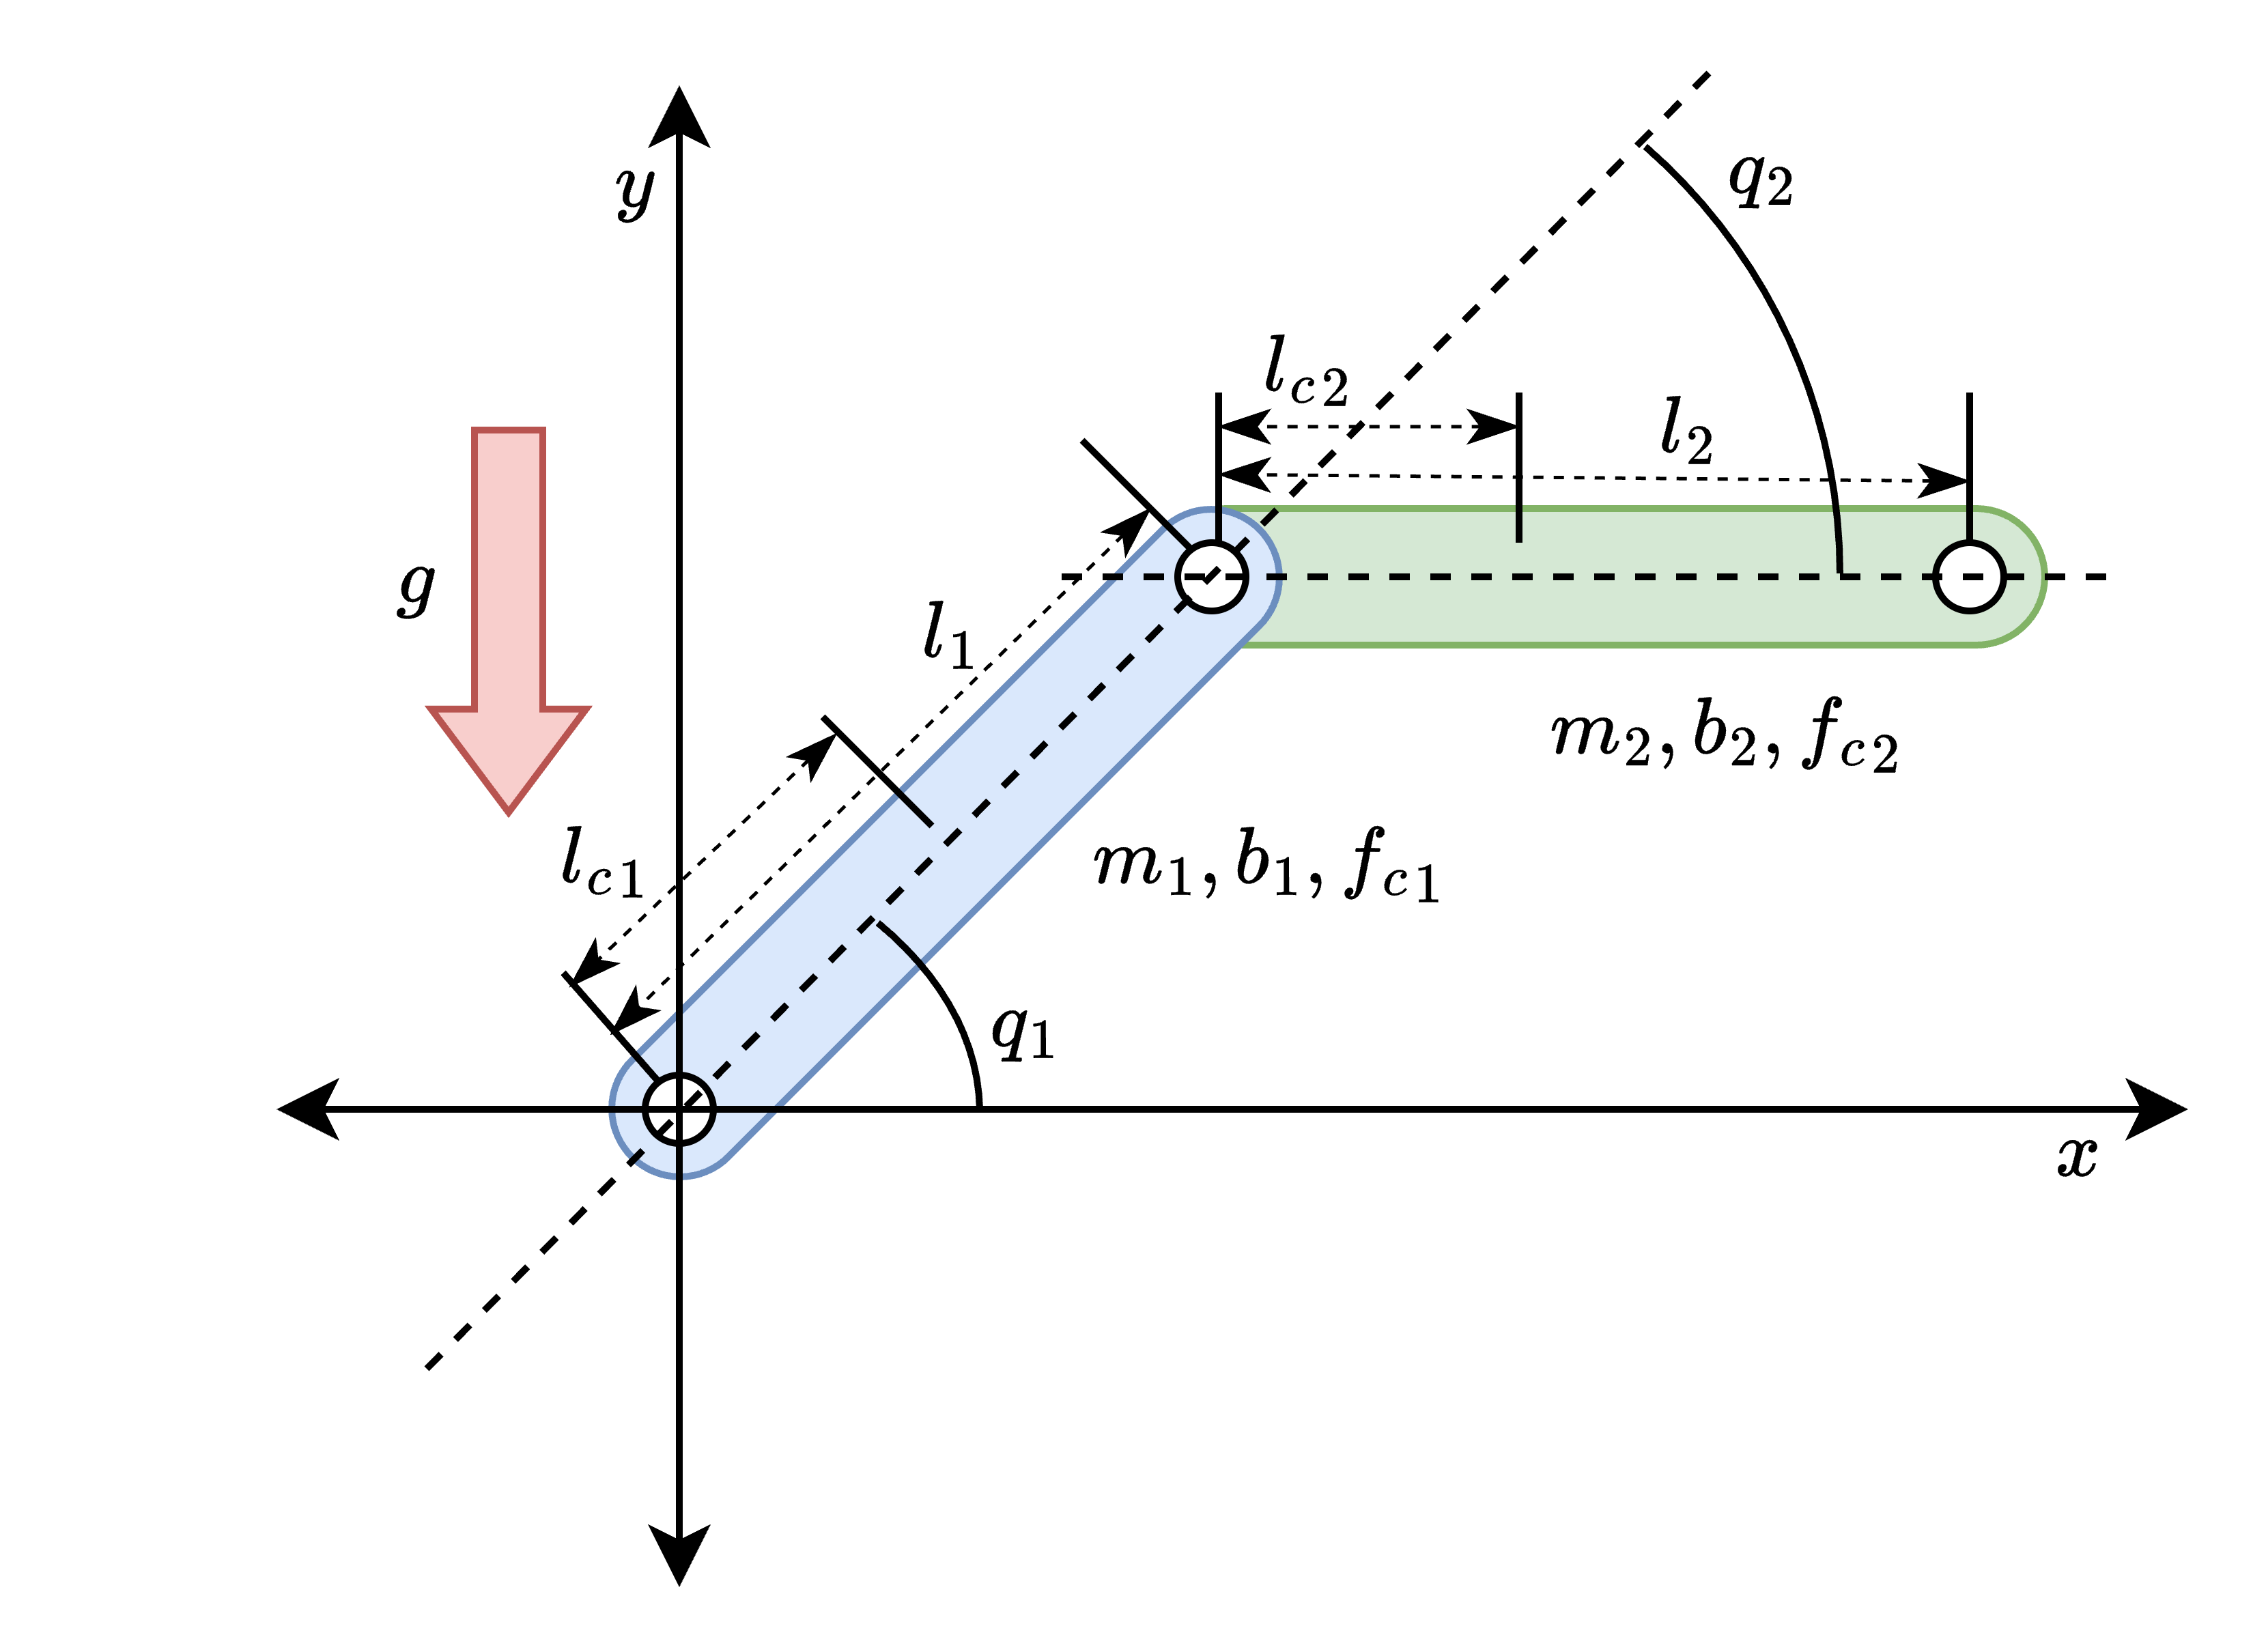
\includegraphics[width=0.75\linewidth]{imgs/RobotModel.drawio.png}
    \caption{Two-link manipulator model.}
    \label{chap3:fig:plant}
\end{figure}

\begin{table}[!t]
    \renewcommand{\arraystretch}{1.3}
    \caption{System model parameters.}
    \centering
    \begin{tabular}{|c||c|c|c|c|}
    \hline
    Symbol & \textbf{Description} & \textbf{Link 1} & \textbf{Link 2} \\
    \hline 
    $m_1, m_2$ & Mass of link    & 23.902 (kg) & 3.88 (kg) \\
    \hline
    $l_1, l_2$  & Length of link   & 0.45 (m) & 0.45 (m) \\
    \hline
    $l_{c1}, l_{c2}$ & COM of link  & 0.091 (m) & 0.048 (m) \\
    \hline
    $\theta_1, b_2$   & Viscous coefficient  &  2.288 (Nms) & 0.172 (Nms) \\
    \hline
    $f_{c1}, f_{c2}$  & Friction coefficient &  7.17 (Nm) & 1.734 (Nm) \\
    \hline
    \end{tabular}
    \label{chap3:table:plant_param}
\end{table}

The two-link manipulator model in \cite{RN33} is employed for the simulation demonstration.
In the system, the parameters $q_p,{q_d}_p,\tau_p,m_p,l_p,{l_c}_p,b_p$, and ${f_c}_p$ denote the joint angle, desired joint angle, torque, mass, length, center of mass, viscous coefficient, and friction coefficient, respectively, for link $p\in[1,2]$.
The values of the system parameters are given in Table~\ref{chap3:table:plant_param}.
The reference signal of the $q=[q_1,q_2]^T$ is defined as follows:
\begin{equation}
    q_d
    =
    \begin{bmatrix}
        {q_d}_1\\
        {q_d}_2
    \end{bmatrix}
    = 
    \begin{bmatrix}
        +\cos(\pi/2 t) + 1 \\
        -\cos(\pi/2 t) - 1 
    \end{bmatrix}
    .
\end{equation}

For the comparative study, three controllers were selected: the neuro-adaptive controller with $L_2$-regularization (NAC-L2) and with $\epsilon$-modification (NAC-eMod), and the proposed controller with constrained optimization (CoNAC).
%%%%%%%%%%%%%%%%%%%%%
The performances of the selected controllers are compared based on the tracking performances and the dependencies of the parameters $\lambda$, $\rho$, and $\beta_j$ of NAC-L2, NAC-eMod, and CoNAC, respectively.
The square root of integrated squared error (ISE) (\ie $\sqrt{\int_0^T\Vert\xi\Vert^2\,dt}$, where $T$ denotes a simulation termination time) is utilized to evaluate the tracking performances.
The parameter dependencies of the controllers were examined via various values of the parameters. 
The values ranged from $0.001$ to $1$ across $10$ samples.
%%%%%%%%%%%%%%%%%%%%%

The control laws of all three controllers were the same as defined in \eqref{chap3:eq:approx_control}.
The adaptation law of NAC-L2 is derived by adding the squared weight term $(1/2)\lambda\hat\theta^T\hat\theta$ to the objective function such that $J_{L_2} = J+(1/2)\lambda\hat\theta^T\hat\theta$, where $\lambda\in\R_{>0}$ denotes the $L_2$-coefficient.
The adaptation law obtained via the gradient descent method is subsequently adjusted by adding stabilizing term $-\alpha\lambda\hat\theta$ as follows:
\begin{equation} 
    \dot{\hat\theta} = 
    {\partial J_{L_2}\over\partial \hat\theta}
    =-\alpha
    \bigg(
        {\partial J\over\partial \hat\theta}+\lambda\hat\theta
    \bigg)
    .
    \label{chap3:eq:adap_L2}
\end{equation}
Note that this adaptation law derived based on $L_2$-regularization method in deep learning is inherently the same as $\sigma$-modification in the adaptive control theory which adds the term $-\alpha\sigma\hat\theta$, where $\sigma\in\R_{>0}$.
For NAC-eMod, Similar to $\sigma$-modification, the stabilizing function $-\alpha\rho\Vert \tilde z \Vert\hat\theta$ is added to the adaptation law as follows:
\begin{equation}
    \dot{\hat\theta} = -\alpha
    \bigg(
        {\partial J\over\partial \hat\theta}+\rho\Vert\tilde z\Vert\hat\theta
    \bigg)
    \label{chap3:eq:adap_eMod}
\end{equation}
where $\rho\in\R_{>0}$ denotes the $\epsilon$-modification coefficient.
By $\Vert\tilde z\Vert$, the stabilizing function proportionally increases as the tracking error $\tilde z$ increases.
Therefore, the adaptation attempts to reduce the tracking error mainly without the effect of the stabilizing function, if the tracking error is sufficiently regulated.
The adaptation law of CoNAC is presented in \eqref{chap3:eq:adap}.
Owing to the stabilizing functions, the weights of NAC-L2 and NAC-eMod are biased, since the stabilizing functions drive the weights toward the origin.

All controllers had the same control parameters except their crucial parameters (\ie $\lambda$, $\rho$ and $\beta_j$) as $k_q=1.1$, $k_z=10$, $M_0=I_2$ and $W=\text{diag}([5,1,15,15])$.
The parameters of the NNs were set $l_0=2$, $l_1=16$, $l_2=2$, and $\alpha=10^3$ and the same random seed was applied for the weight initialization.
The NN input vector was set to the desired trajectory $q_d$, with the augmented 1 to incorporate the bias term in the weight matrix, such that $q_{NN}=[q_d^T,1]^T$. 
For CoNAC, the parameters of the weight norm constraints were set as $\bar\theta_0=10$ and $\bar\theta_1=20$.
The sampling time of the simulation and the simulation termination time were set to $T_s=10^{-4}$ and $T=10$, respectively.

\subsection{Results}

\begin{figure}[!t]      
    \centering
    {\includegraphics[width=.85\linewidth]{imgs/BoxWhisker.drawio.png}}
    \caption{
        Box-and-Whisker plot of the square root of the tracking ISEs of NAC-L2, NAC-eMod and CoNAC across various parameter values.
    }
    \label{chap3:fig:box-whisker}
\end{figure}

\begin{table}[!t]
    \renewcommand{\arraystretch}{1.3}
    \caption{Quantitative comparison of square root of tracking ISE.}
    \centering
    \begin{tabular}{|c||c|c|c|}
    \hline
     & \textbf{NAC-L2} & \textbf{NAC-eMod} & \textbf{CoNAC} (proposed) 
     \\
    \hline 
    Maximum         & $11.1753$e-3 & $0.5603$e-3 & $0.3439$e-3 \\
    \hline
    Upper quartile  & $1.7284$e-3 & $0.5566$e-3 & $0.3261$e-3 \\
    \hline
    Median          & $0.5898$e-3 & $0.5519$e-3 & $0.3240$e-3 \\
    \hline
    Lower quartile  & $0.5533$e-3 & $0.5470$e-3 & $0.3238$e-3 \\
    \hline
    Minimum         & $0.5434$e-3 & $0.5434$e-3 & $0.3235$e-3 \\
    \hline
    \end{tabular}
    \label{chap3:table:error_norm}
\end{table}

As shown in Fig.~\ref{chap3:fig:box-whisker}, the maximum square root of tracking ISE of CoNAC is smaller than the minimum square root of tracking ISEs of NAC-L2 and NAC-eMod for all variations of the parameters.
This is because NAC-L2 and NAC-eMod bias the weights to the origin, due to the presence of the stabilizing functions.
A quantitative comparison of the square root of tracking ISE is provided in Table~\ref{chap3:table:error_norm}.

\begin{figure}[!t]      
    \centering
        \subfloat[NAC-L2]{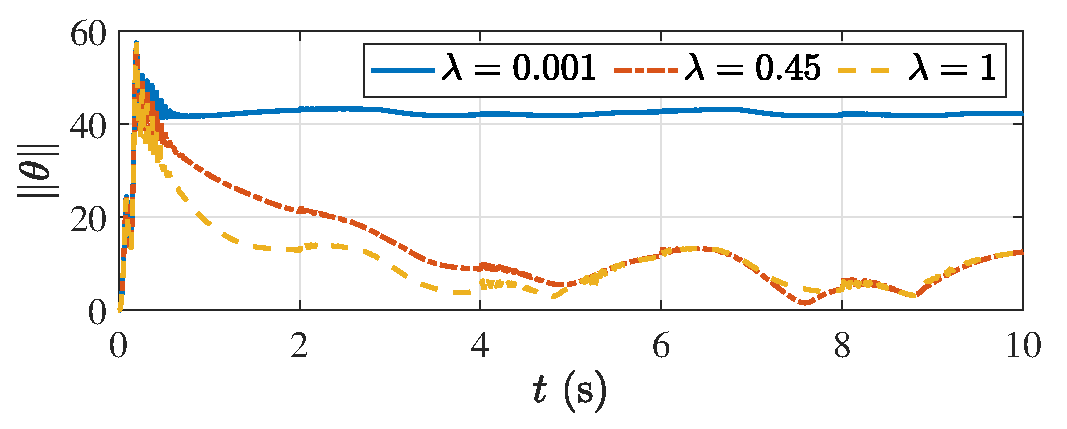
\includegraphics[width=.85\linewidth]{imgs/Chap3/fig9.eps}%
        \label{chap3:fig:weight_NAC-L2}}
    \vfill
        \subfloat[NAC-eMod]{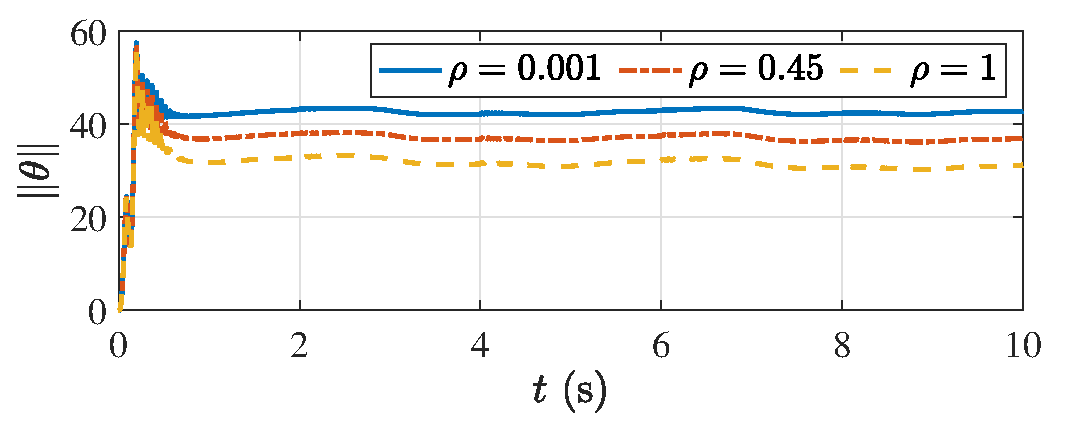
\includegraphics[width=.85\linewidth]{imgs/Chap3/fig10.eps}%
        \label{chap3:fig:weight_NAC-eMod}}
    \vfill
        \subfloat[CoNAC]{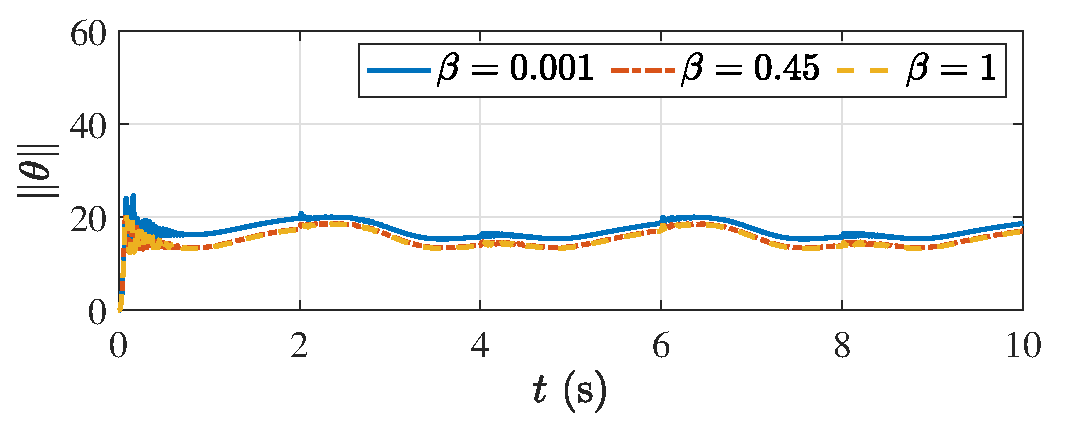
\includegraphics[width=.85\linewidth]{imgs/Chap3/fig8.eps}%
        \label{chap3:fig:weight_CoNAC}}
    \vfill
    \caption{Weight norms of NAC-L2, NAC-eMod and CoNAC.}
    \label{chap3:fig:weight}
\end{figure}

\begin{figure}[!t]      
    \centering
        \subfloat[NAC-L2]{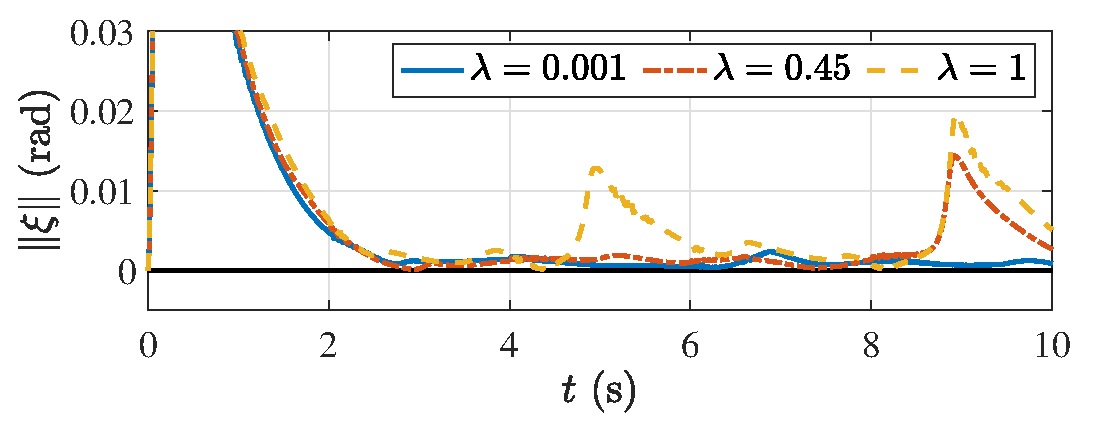
\includegraphics[width=.85\linewidth]{imgs/Chap3/fig6.eps}%
        \label{chap3:fig:error_NAC-L2}}
    \vfill
        \subfloat[NAC-eMod]{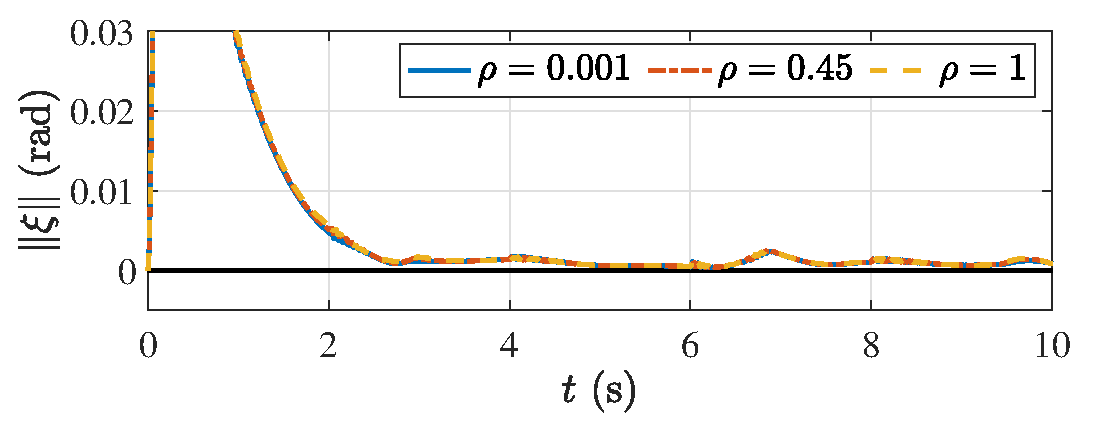
\includegraphics[width=.85\linewidth]{imgs/Chap3/fig7.eps}%
        \label{chap3:fig:error_NAC-eMod}}
    \vfill
        \subfloat[CoNAC]{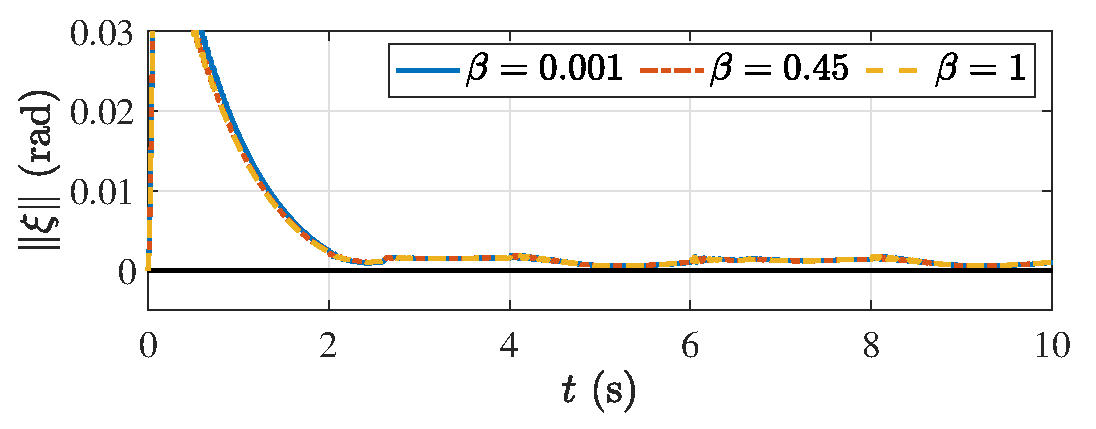
\includegraphics[width=.85\linewidth]{imgs/Chap3/fig5.eps}%
        \label{chap3:fig:error_CoNAC}}
    \vfill
    \caption{Tracking errors of NAC-L2, NAC-eMod and CoNAC.}
    \label{chap3:fig:error}
\end{figure}

For the detailed analysis, three values of the parameters (\ie $\lambda,\rho,\beta_j\in[0.001,0.45,1] \allowbreak $) were selected as described in Fig.~\ref{chap3:fig:weight} and Fig.~\ref{chap3:fig:error}.
As shown in Fig.~\ref{chap3:fig:weight_NAC-L2}, increasing $\lambda$ reduces the weight norm of NAC-L2 by the stabilizing function $-\alpha\lambda\hat\theta$.
Moreover, the high dependency of NAC-L2 to the $L_2$-regularization coefficient $\lambda$ also can be observed.
Since the weight norm is decreased, NAC-L2 cannot generate sufficient control inputs, resulting in a larger square root of tracking ISE, as shown in Fig.~\ref{chap3:fig:error_NAC-L2}.

On the other hand, NAC-eMod exhibits lower dependency on the $\epsilon$-modification coefficient $\rho$ as shown in Fig.~\ref{chap3:fig:weight_NAC-eMod} and Fig.~\ref{chap3:fig:error_NAC-eMod}.
This is because stabilizing function $-\alpha\rho\Vert\tilde z\Vert\hat\theta$ can be decreased once the tracking error $\tilde z$ is sufficiently regulated.
However, the bias of the weights to the origin still exists as described in Fig.~\ref{chap3:fig:weight_NAC-eMod} (\ie smaller weight norms are observed as $\rho$ is increased.).
Therefore, similar to NAC-L2, the biased weights produce insufficient control input, resulting in a relatively larger square root of tracking ISE than that of CoNAC, as described in Table \ref{chap3:table:error_norm}.

Finally, the weight norm of CoNAC is smaller than those of NAC-L2 and NAC-eMod as shown in Fig.~\ref{chap3:fig:weight_CoNAC} with better tracking performances.
Even if the large $\beta_j$ is provided, CoNAC can adjust the adaptation direction to satisfy the weight norm constraints faster, according to \eqref{chap3:eq:adap_L}.
Therefore, the lowest dependency on the update rate $\beta_j$ is observed in CoNAC as shown in Fig.~\ref{chap3:fig:weight_CoNAC} and Fig.~\ref{chap3:fig:error_CoNAC}.
Note that $\beta_j$ of CoNAC is the update rate for Lagrange multipliers while $\lambda$ and $\rho$ are the coefficients of the stabilizing function that generates the biases of the weights.
However, considering the implementation using a digital computer, excessively large $\beta_j$ should be avoided.

The details of the satisfaction of the weight norm constraints are shown in Fig.~\ref{chap3:fig:weight_multiplier CoNAC} for CoNAC with $\beta_j=0.001$.
As the weight norms of each layer reach the constraint boundary, the corresponding Lagrange multipliers are generated.
Using the Lagrange multipliers, the adaptation direction is adjusted toward the constraint satisfactory point.
The Lagrange multipliers disappear when the constraints are satisfied, and the weights are adapted to optimize the original objective function without weight bias.

\begin{figure}[!t]      
    \centering
    \subfloat[Weight norm]{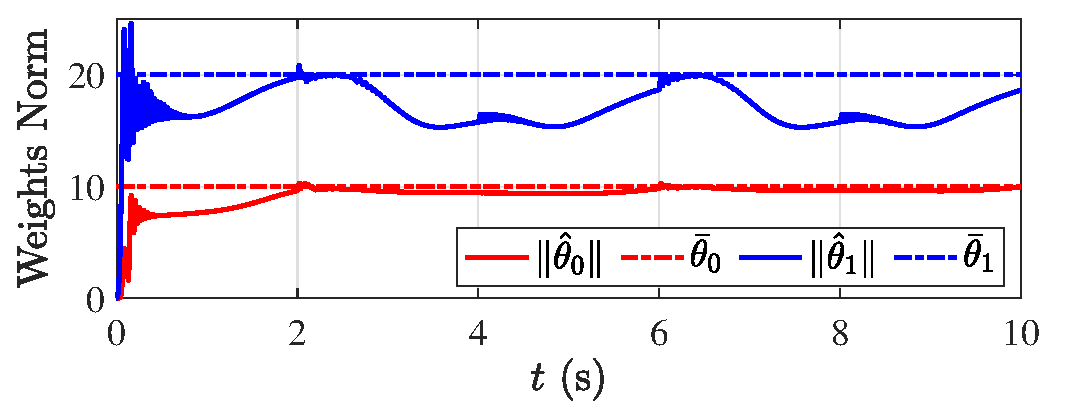
\includegraphics[width=.85\linewidth]{imgs/Chap3/fig12.eps}%
    \label{chap3:fig:weight_norms CoNAC}}
    \vfill
    \subfloat[Lagrange multipliers]{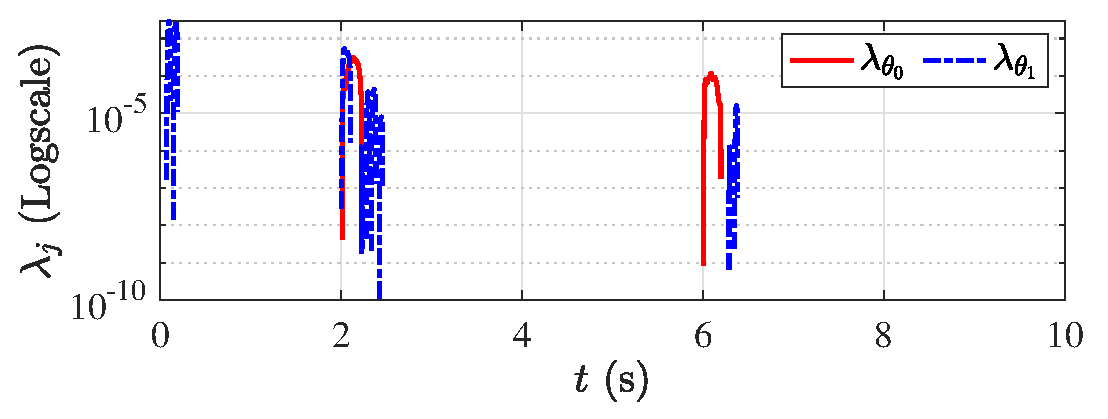
\includegraphics[width=.85\linewidth]{imgs/Chap3/fig11.eps}%
    \label{chap3:fig:multipliers CoNAC}}
    \caption{Weight norms and Lagrange multipliers of CoNAC ($\beta=0.001$).}
    \label{chap3:fig:weight_multiplier CoNAC}
\end{figure}

Furthermore, it is important to note that CoNAC shows enhanced tracking performance with smaller weights than NAC-L2 and NAC-eMod.
This implies that the weights in CoNAC approach the different local optimal solution points from those of NAC-L2 and NAC-eMod.
Therefore, if the physical analysis of the system is available to predict the feasible maximum control inputs, CoNAC can find the local optimal solution without unnecessary large control input by imposing the proper weight norm constraints.

%%%%%%%%%%%%%%%%%%%%%%%%%%%%%%%%
\section{Conclusion}
%%%%%%%%%%%%%%%%%%%%%%%%%%%%%%%%

In this chapter, a Constrained Optimization-based Neuro-Adaptive Controller \allowbreak (CoNAC) with a single hidden layer neural network (SHLNN) and weight norm constraint is presented for the uncertain Euler-Lagrange systems.
The boundedness of the weights is handled by formulating a constrained optimization problem with weight norm inequality constraints.
Using the constrained optimization approach, the adaptation laws of the weights and Lagrange multipliers are derived.
The boundedness of the tracking error and the weight estimation are analyzed via Lyapunov analysis.
The simulation results demonstrated that the proposed controller outperforms the existing methods in terms of tracking performance and parameter dependency.
In next chapter, CoNAC will be extended to handle input constraints and DNN.



\end{spacing}

%%%%%%%%%%%%%%%%%%%%%%%%%%%%%%%%%%%%
% Chapter 4
%%%%%%%%%%%%%%%%%%%%%%%%%%%%%%%%%%%%

% \begin{spacing}{2.0} % double spacing
\begin{spacing}{1.3} % double spacing
%%%%%%%%%%%%%%%%%%%%%%%%%%%%%%%%
% Chap 4. Constrained Optimization-Based Neuro-Adaptive Control (CoNAC) for Uncertain Euler–Lagrange Systems Under Weight and Input Constraints
%%%%%%%%%%%%%%%%%%%%%%%%%%%%%%%%

\chapter{
    CoNAC for Uncertain Euler–Lagrange Systems Under Weight and Input Constraints
} \label{chapter4}

%%%%%%%%%%%%%%%%%%%%%%%%%%%%%%%%
\section{Introduction}
%%%%%%%%%%%%%%%%%%%%%%%%%%%%%%%%

Besides the boundedness of neural network (NN) weights, the other major issue is satisfying input constraints, particularly in systems where actuators are subject to physical limitations \cite{RN24}. 
The unpredictable outputs of NNs can sometimes lead to excessively large control inputs which may destroy the actuators or the system itself. 
This problem is exacerbated in neuro-adaptive controllers (NACs) that attempt to cancel out system dynamics using conventional methods like feedback linearization or backstepping. 
In such cases, controllers may produce overly aggressive control inputs, even when the system's natural dynamics are stabilizing, leading to unnecessary saturation of the control inputs.

In this chapter, the Constrained Optimization-based Neuro-Adaptive Controller (CoNAC) framework is extended to address the input saturation problem.
Moreover, single hidden layer neural network (SHLNN) is substituted by deep neural network (DNN).

%%%%%%%%%%%%%%%%%%%%%%%%%%%%%%%%
\section{Problem formulation} \label{chap4:problem}
%%%%%%%%%%%%%%%%%%%%%%%%%%%%%%%%

Consider an uncertain Euler–Lagrange system modeled as
\begin{equation}
    M(q)\ddot q + C(q,\dot q)\dot q + G(q) + F(q) = h(\tau)
    \label{chap4:eq:sys1}
\end{equation}
where $q\in \R^n$ denotes the generalized coordinate, and $\tau\in\R^n$ denotes the control input. The terms $M(q)\in\R^{n\times n}$, $C(q,\dot q)\in\R^{n\times n}$, and $G(q)\in\R^{n}$ represent the unknown system function matrices, while $F(q)\in\R^{n}$ denotes the external force. The function $h(\cdot)\in \R^n$ is a control input saturation function, where each element represents the control input saturation for each element of $\tau$. The gradient of $h(\cdot)$ with respect to $\tau$ is continuous and bounded, \ie $\Vert\partial h/\partial \tau\Vert_F\in L_\infty$. 

The control input saturation function represents the inherent physical limitations of the actuators. To account for these limitations, it is essential to incorporate physically motivated constraints into the controller design. Section \ref{chap4:sec:cstr_candidates} introduces candidate constraints that can be applied to ensure compliance with these physical limitations.

Using user-designed nominal system matrices $M_0 > 0$, $C_0$, and $G_0$, \eqref{chap4:eq:sys1} can be reformulated as
\begin{equation}
    M_0\ddot q+C_0\dot q+G_0 = h(\tau) + f(q,\dot q,\ddot q)
    \label{chap4:eq:sys2}
\end{equation}
where $f(q,\dot q,\ddot q) \triangleq -\Delta M(q)\ddot q-\Delta C(q,\dot q)\dot q -\Delta G(q) -F(q)\in\R^n$ is the lumped system uncertainty function. Here, $\Delta M(q)\triangleq M(q)-M_0$, $\Delta C(q,\dot q)\triangleq C(q,\dot q)-C_0$, and $\Delta G(q)\triangleq G(q)-G_0$. 

The function $f$ acts like an external disturbance, leading to a poor performance index and potential instability. 
%Therefore, an adaptive control approach is required to improve the control performance. 
The control objective is to develop a neuro-adaptive controller that enables $q$ to track a continuously differentiable desired trajectory ${q_d}(t): \R \to \R^n$, compensating for the unknown function $f$ while addressing the imposed constraints (\eg weight boundedness and input saturation).

%%%%%%%%%%%%%%%%%%%%%%%%%%%%%%%%
\section{Existing Works to Prevent Input Saturation} 
%%%%%%%%%%%%%%%%%%%%%%%%%%%%%%%%

To address input saturation, one may consider the projection operator in Section \ref{chap3:sec:proj} as one of solutions.
However, the projection operator can not be simply applied since the NNs are highly nonlinear and non-convex function.
Note that the operator is used to project on given convex set.

On the other hand, many studies introduced auxiliary systems. These systems mitigated the effects of control input saturation by modifying the control strategy when saturation occurred. 
For instance, in \cite{RN60, RN95, RN46}, auxiliary states were generated whenever input saturation was detected, and these states were incorporated into the adaptation law to adjust the NN weights accordingly. 
For details, the auxiliary systems are generally designed as
\begin{equation}
    \dot\zeta = A_\zeta \zeta + B_\zeta \Delta\tau
\end{equation}
where $\zeta$ is the auxiliary state, $A_\zeta$ is Hurwitz matrix, $B_\zeta$ is control gain matrix, and $\Delta\tau_{(i)}=\tau_{(i)}-\tau_{\text{sat},(i)}$ is saturated control input of each control channel where $\tau_{\text{sat},(i)}$ denote maximum or minimum value of $\tau_{(i)}$.
Thus, the auxiliary state $\zeta$ is generated when the control input $\tau$ exceeds the saturation limit $\tau_{\text{sat}}$.
Using the auxiliary state, the feedback signal for the adaptation law is modified as
\begin{equation}
    \dot{\hat\theta} = \gamma(\xi) 
    \ \to \ 
    \dot{\hat\theta}=\gamma(\xi+\zeta)
\end{equation}
where $\gamma(\cdot)$ denotes arbitrary adaptation law and $\xi$ denotes tracking error which is typically used as feedback signal for adaptation process for NACs.  
This approach helped the controller reduce input saturation by indirectly regulating the auxiliary states.
Alternatively, auxiliary states can also be used as feedback terms in the control law to directly compensate for the effects of input saturation constraints, as demonstrated in \cite{RN89, RN88, RN82}. 
In \cite{RN18}, the NN was used to approximate the desired control input, compensating for input saturation. 

However, these approaches typically handle input bound constraints on a per-input basis (\ie applying bounds to each scalar control variable individually), and may not account for more complex, nonlinear constraints, like input norm constraints, which are commonly found in physical systems such as robotic actuators or motor systems.

%%%%%%%%%%%%%%%%%%%%%%%%%%%%%%%%
\section{CoNAC with Weight and Input Constraints}
%%%%%%%%%%%%%%%%%%%%%%%%%%%%%%%%

The architecture of the proposed CoNAC is illustrated in Fig.~\ref{chap4:fig:ctrl}, consisting of: a reference generator, a DNN that functions as a neuro-adaptive controller, and a weight optimizer for the DNN. 
The simple version of the CoNAC is introduced in Section \ref{chap3:sec:ctrl_dev} ahead with the SHLNN instead of the DNN and the weight norm constraints.
We will extend it to the DNN with the weight and input constraints in this chapter.

\begin{figure*}[t]
    \centering
    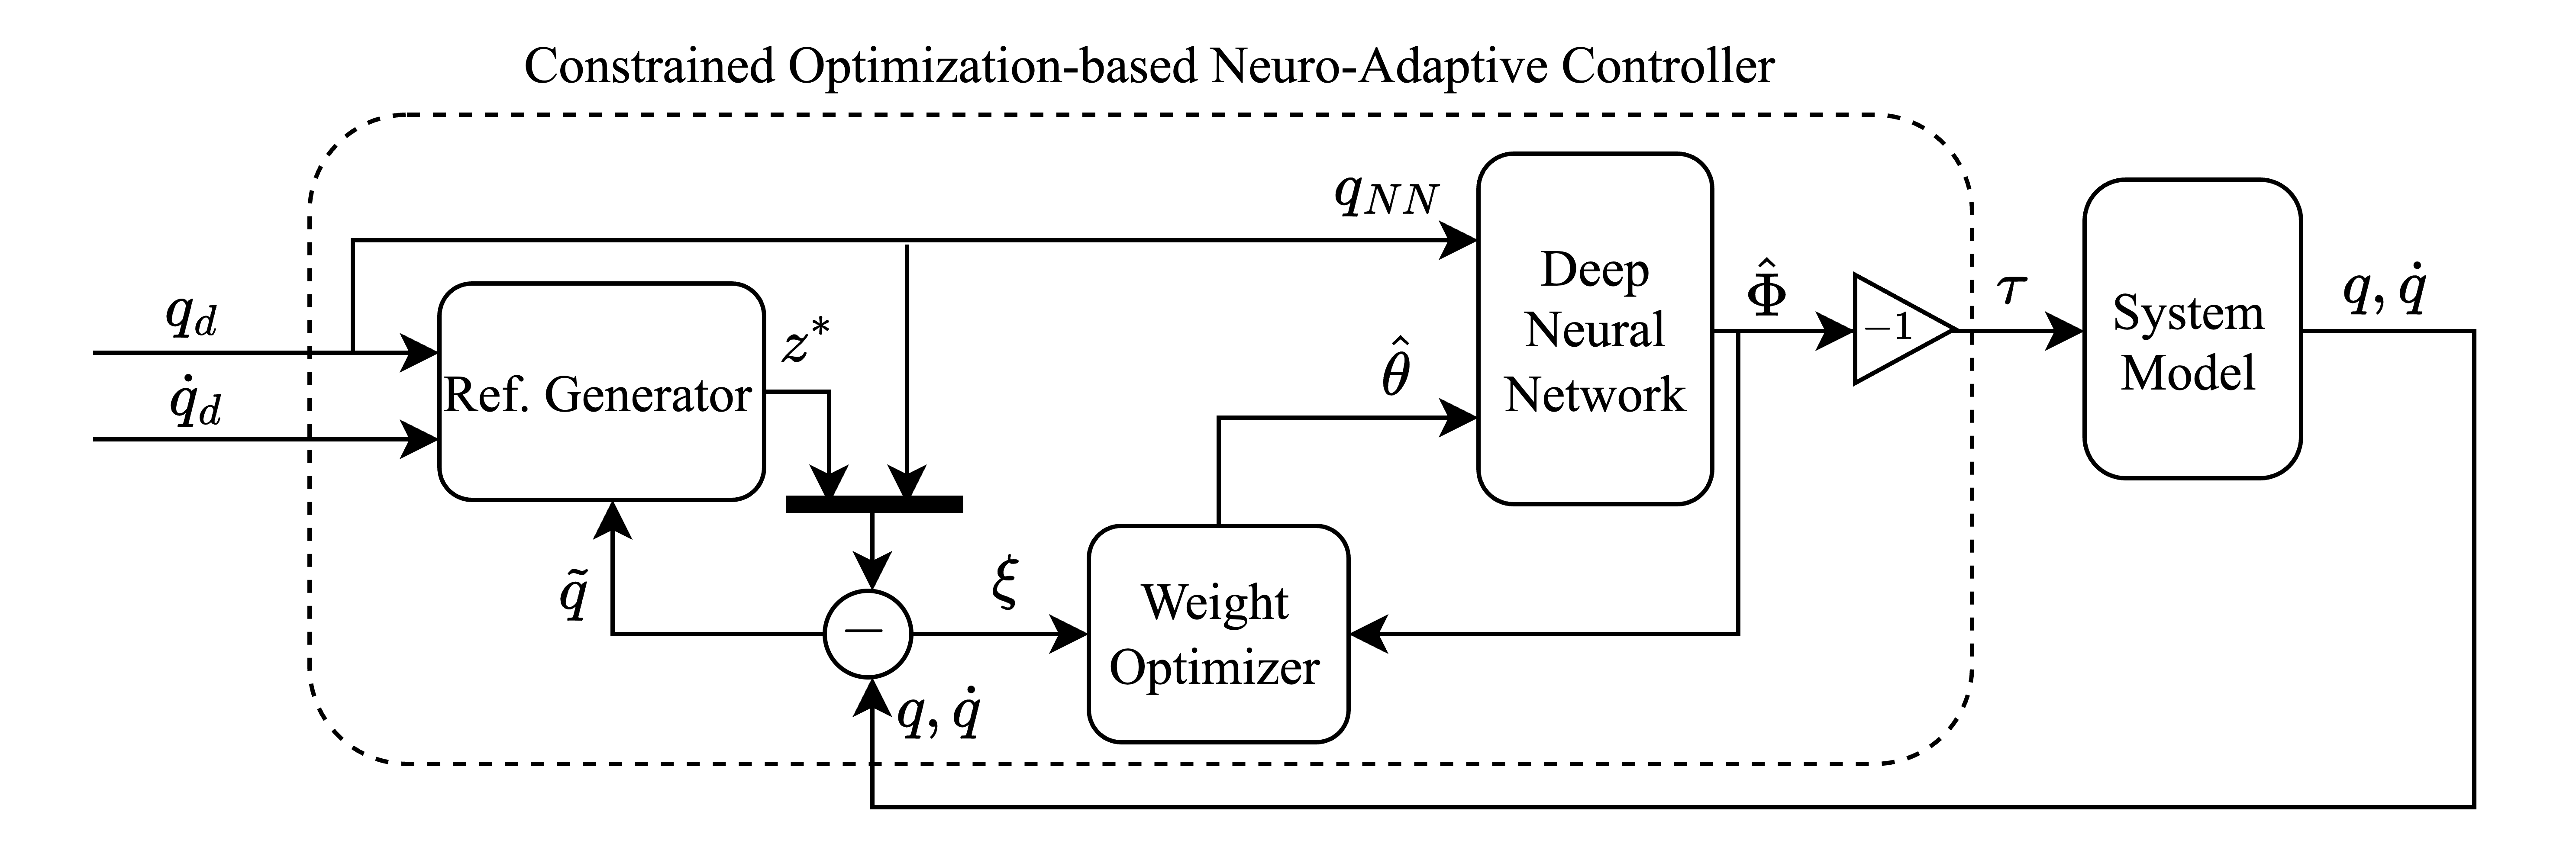
\includegraphics[width=0.9\linewidth]{imgs/ControllerChap4.drawio.png}
    \caption{Architecture of the Constrained Optimization-based Neuro-Adaptive Controller (CoNAC).}
    \label{chap4:fig:ctrl}
\end{figure*}

\subsection{Control Law Development}

The system dynamics \eqref{chap4:eq:sys2} can be represented as
\begin{equation}
    \begin{aligned}
        \dot {q} &= {z},\\
        \dot {z} &= -M_0^{-1} C_0 {z}-M_0^{-1} G_0+M_0^{-1} h(\tau) + M_0^{-1} f,
    \end{aligned}
    \label{chap4:eq:x_dyna}
\end{equation}
where ${z}\triangleq \dot q$.

Similar to the control law development in Section \ref{chap3:sec:ctrl_dev}, the reference generator generates the desired trajectory $z^*\triangleq -k_q\tilde q+\dot q_d$ for $z\triangleq \dot q$, where $\tilde q\triangleq q-q_d$ and $k_q\in\R_{>0}$.
Then the desired stabilizing controller can be designed As
\begin{equation}
    \tau^* = -M_0(k_z\tilde z+\tilde q)+C_0 z+G_0-f+M_0\dot z^*
    \label{chap4:eq:desired_control}
\end{equation}
where $\tilde z\triangleq z-z^*$, $k_z\in\R_{>0}$, and $k_z\in\R_{>0}$.
Note that the control law $\tau^*$ cannot be realized because of $f$.

The DNN is defined as 
\begin{equation}
    \Phi(q_{NN};\theta) \triangleq 
    \underbrace{
        V_k^T  \phi_{k}(
        \underbrace{
        V_{k-1}^T   \cdots \phi_2(
        \underbrace
            {
            V_1^T   \phi_1(
            \underbrace
            {
            V_0^T   q_{NN}
            }_{\Phi_0}
            )
        }_{\Phi_1}
        )\cdots )
        }_{\Phi_{k-1}}
        )
    }_{\Phi_k}
\end{equation}
where $q_{NN}$ denotes the NN input vector, $V_i\in\R^{(l_i+1)\times l_{i+1}}$ is the weight matrix of the $i\textsuperscript{th}$ layer, and $\phi_i: \R^{l_i}\to\R^{l_i+1}$ represents the activation function of the $i\textsuperscript{th}$ layer.
For the simplicity, the weights are vectorized in $\theta\triangleq[\theta_i]_{i\in[k,\cdots,0]}\in\R^{\Xi}$ consisting of vectorized weights of each layer such that $\theta_i\triangleq\text{vec}(V_i)\in\R^{\Xi_i}$, where $\Xi\triangleq \sum_{i\in[k,\cdots 0]}$ denotes the total number of weights and $\Xi_i\triangleq (l_i+1)l_{i+1}$ denote the number of weights in the $i\textsuperscript{th}$ layer, respectively.
The details of the DNN architecture is provided in Section \ref{chap2:sec:DNN}.

According to Theorem \ref{chap2:thm:uni_approx}, $\Phi(q_{NN};\theta)$ can approximate a nonlinear function $g(\cdot)$ with an ideal weight vector $\theta^*$ on a compact subset $\Omega_{NN}\in\R^{l}$ to $\epsilon$-accuracy, such that $\sup_{q_{NN}\in\Omega_{NN}}\Vert \Phi(q_{NN};\theta^*) - g(\cdot) \Vert = \epsilon < \infty$.
The ideal weight $\theta^*$ is typically assumed to be bounded, \ie $\Vert\theta^*\Vert\le \bar\theta<\infty$.
In this thesis, $\theta^*$ is defined as a local optimal point, rather than a global optimal point.

Therefore, the desired control law is expressed by the DNN approximation with the ideal weight vector $\Phi^*\triangleq\Phi(q_{NN};\theta^*)$ as follows:
\begin{align}
    \tau^*=& -(\Phi^*+\epsilon),
\end{align}
which is estimated online by
\begin{align}
    \tau =& -\hat\Phi,
    \label{chap4:eq:approx_control}
\end{align}
where $\hat\Phi\triangleq\Phi(q_{NN};\hat\theta)$, and  $\hat\theta$ is the estimated weight vector for $\theta^*$.

Using \eqref{chap4:eq:x_dyna}, \eqref{chap4:eq:desired_control}, \eqref{chap4:eq:approx_control}, and the definition of $\tilde z$ the error dynamics can be derived as
\begin{equation}
    \begin{aligned}
        \dot {\tilde q} = & -{k_q} {\tilde q} + {\tilde z} \\
        \dot {\tilde z} = & -{\tilde q} -{k_z} {\tilde z} + M_0^{-1} (\Phi^*-h(\hat\Phi)+\epsilon).
    \end{aligned}
    \label{chap4:eq:e_dyna}
\end{equation}
The error dynamics \eqref{chap4:eq:e_dyna} can be represented as a first-order system: 
\begin{equation}
    \dot\xi = A_\xi \xi + B_\xi (\Phi^*-h(\hat\Phi)+\epsilon)
    \label{chap4:eq:xi_dyna}
\end{equation}
where 
$\xi\triangleq[{\tilde q}^T  , {\tilde z}^T  ]^T  \in\R^{2n}$ denotes the augmented error,
and
\begin{equation}
    A_\xi \triangleq 
    \begin{bmatrix}
        -{k_q} I_n &I_n\\-I_n& -{k_z} I_n
    \end{bmatrix}
    ,\ 
    B_\xi \triangleq 
    \begin{bmatrix}
        0_{n\times n}\\M_0^{-1}
    \end{bmatrix}.
\end{equation}
Note that $A_\xi$ is a stable matrix, and $\Vert B_\xi\Vert_F<\infty$.
For further sections, $\phi^*_i \triangleq\phi_i(\Phi^*_{i-1})$ and ${\phi^*}'_i = \partial \phi^*_i/\partial \Phi^*_{i-1}$, and $\hat\phi_i \triangleq\phi_i(\hat\Phi_{i-1})$ and $\hat\phi_i' = \partial \hat\phi_i/\partial \hat{\Phi}_{i-1}$.

%%%%%%%%%%%%%%%%%%%%%%%%%%%%%%%%
\subsection{Weight Adaptation Laws}
%%%%%%%%%%%%%%%%%%%%%%%%%%%%%%%%

The adaptation laws are same to the previous Section \ref{chap3:sec:weight_adap} and represented as follows:
%\begin{equation}
\begin{align}
    \dot {\hat\theta}&=-\alpha {\partial L\over\partial \hat\theta}
    =-\alpha 
    \bigg(
    {\partial J\over \partial \hat\theta}+\sum_{j\in\mathcal{A}}
    \lambda_j {\partial c_j\over\partial \hat\theta}
    \bigg),
\label{chap4:eq:adap_th}
    \\
    \dot\lambda_j& = \beta_j{\partial L\over\partial \lambda_j} = \beta_j c_j ,
    \quad\quad\quad\quad      \      
    \forall j\in\mathcal A,
\label{chap4:eq:adap_L}
    \\
    \lambda_j & = \max(\lambda_j,0) ,
    \quad\quad\quad\quad\ \ \ \ \ 
    \forall j\in\mathcal A,
\label{chap4:eq:adap_L_max}
\end{align}
% \end{equation}
where $L\triangleq J(\xi;\hat\theta)+\sum_{j\in\mathcal A}\lambda_j c_j(\hat\theta)$ denotes Lagrangian function consisting of the original objective function $J\triangleq(1/2)\xi^T\xi$, the inequality constraint $c_j,\ j\in\mathcal I$ and Lagrange multiplier $\lambda_j$, where $\mathcal I$ is the set of imposed constraints, $\mathcal A \triangleq \{j\in\mathcal I\ |\ c_j\ge 0\}$ represents the active set.
Moreover, $\alpha\in\R_{>0}$ denotes the adaptation gain (learning rate) and $\beta_j\in\R_{>0}$ denotes the update rate of the Lagrange multipliers in $\mathcal A$. 

%%%%%%%%%%%%%

Using the chain rule, the gradient of the objective function with respect to the weights (\ie $\partial J/\partial \hat\theta$) in \eqref{chap4:eq:adap_th} can be represented as
\begin{equation}
    {\partial J\over\partial \hat\theta}
    =
    {\partial \xi\over\partial \hat\theta}^TW
    {\partial \xi\over\partial \hat\theta}
    .
\end{equation}
Using the forward sensitivity method presented in \cite{RN49}, the sensitivity equation can be obtained as follows:
\begin{equation}
    \dot \eta =A_\xi - B_\xi {\partial \hat\Phi\over\partial \hat\theta}
    \label{chap4:eq:eta_dyna}
\end{equation}
where $\eta\triangleq \partial \xi/\partial \hat\theta\in\R^{2n\times \Xi}$ denotes the sensitivity of the weights to the augmented error.
The initial value of $\eta$ is zero since the initial $\xi$ is independent of the weights.
By decomposing for each layer, the dynamics of $\eta_i\triangleq \partial \xi/\partial \hat\theta_i\in\R^{2n\times \Xi_i}$ can be represented as
\begin{equation}
    \begin{aligned}
        \dot \eta&= 
        \begin{bmatrix}
            \eta_k&
            \eta_{k-1}&
            \cdots &
            \eta_0
        \end{bmatrix}'
        \\
        &=A_\xi
        \begin{bmatrix}
            \eta_k&
            \cdots &
            \eta_0
        \end{bmatrix}
        -B_\xi{\partial h\over\partial \tau}
        \begin{bmatrix}
            (I_{l_{k+1}}\otimes \hat\phi_{k}^T  )&
        \cdots&
        (\cdot)
        \end{bmatrix}
    \end{aligned}
\end{equation}
The calculation of $\partial \hat\Phi/\partial\hat\theta$ is presented in \eqref{chap2:eq:DNNgrad}.
In conclusion, by simulating the sensitivity equation \eqref{chap4:eq:eta_dyna} the gradient of the objective with respect to the weights can be obtained as follows:
\begin{equation}
    {\partial J\over\partial\hat\theta}
    =
    \begin{bmatrix}
        \partial J/\partial\hat\theta_k\\\vdots\\\partial J/\partial\hat\theta_0\\
    \end{bmatrix}    =
    \begin{bmatrix}
        \eta_k^T\\\vdots\\\eta_0^T\\
    \end{bmatrix}
    W
    \xi
\end{equation}

The adaptation is implemented using Algorithm \ref{chap4:alg:alg1}. For implementation in the discrete-time domain, it is recommended to use a sufficiently small sampling time $T_s$. If a large $T_s$ is used, $\alpha$ and $\beta_j$ should satisfy the Armijo condition \cite[Chap.~3 eq.~(3.4)]{RN9} to ensure that the objective function decreases.

\begin{algorithm}[t]
    \caption{Weight Optimizer Implementation.}\label{chap4:alg:alg1}
    \SetKwInOut{Input}{input}
    \SetKwInOut{Output}{output}
        \Input{$\xi$, $\hat\theta$, $\lambda_j$, $\eta$}
        \Output{$\hat\theta$, $\lambda_j$, $\eta$}
        \BlankLine
        \emph{Set $\mathcal A \leftarrow \mathcal A\cup \{j\}$ for all $c_j\ge0$}\;
        \emph{Determine update matrix $\dot\eta$ using \eqref{chap4:eq:eta_dyna}}\;
        \emph{Update $\eta\leftarrow \eta +\dot\eta\cdot T_s$}\; 
        \emph{Determine update directions $\dot{\hat\theta}$, $[\dot\lambda_j]_{j\in\mathcal A}$ using \eqref{chap4:eq:adap_th}, \eqref{chap4:eq:adap_L}}\;
        \emph{Update weight vector $\hat\theta\leftarrow \hat\theta+\dot{\hat\theta}\cdot T_s$}\;
        \emph{Update multipliers $[\lambda_j]_{j\in\mathcal A}\leftarrow [\lambda_j]_{j\in\mathcal A}+[\dot\lambda_j]_{j\in\mathcal A}\cdot T_s$}\;
        \emph{$[\lambda_j]_{j\in\mathcal A}\leftarrow \max([\lambda_j]_{j\in\mathcal A}, 0)$}\;
        \emph{Set $\mathcal A \leftarrow \mathcal A - \{j\}$ for all $\lambda_j=0$}\;
\end{algorithm}

%%%%%%%%%%%%%%%%%%%%%%%%%%%%%%%%
\section{Constraint Candidates} \label{chap4:sec:cstr_candidates}
%%%%%%%%%%%%%%%%%%%%%%%%%%%%%%%%

This section introduces potential weight and input constraints that can be used in the CoNAC. The controller can handle any combination of the following constraints, provided they meet the specified assumptions.

\begin{assumption}
    The constraint functions $c_j(\hat\theta),\ \forall j\in\mathcal I$ are convex in the $\tau$-space and satisfy $c_j(0) \le 0$ and $c_j(\theta^*)\le 0$.
    \label{chap4:assum:assum1}
\end{assumption}

\begin{assumption}
    The selected constraints satisfy the Linear Independence Constraint Qualification (LICQ).
    \label{chap4:assum:assum2}
\end{assumption}

\subsection{Weight Norm Constraint} \label{chap4:sec:weight_cstr}

\begin{figure*}[t]
    \centering
    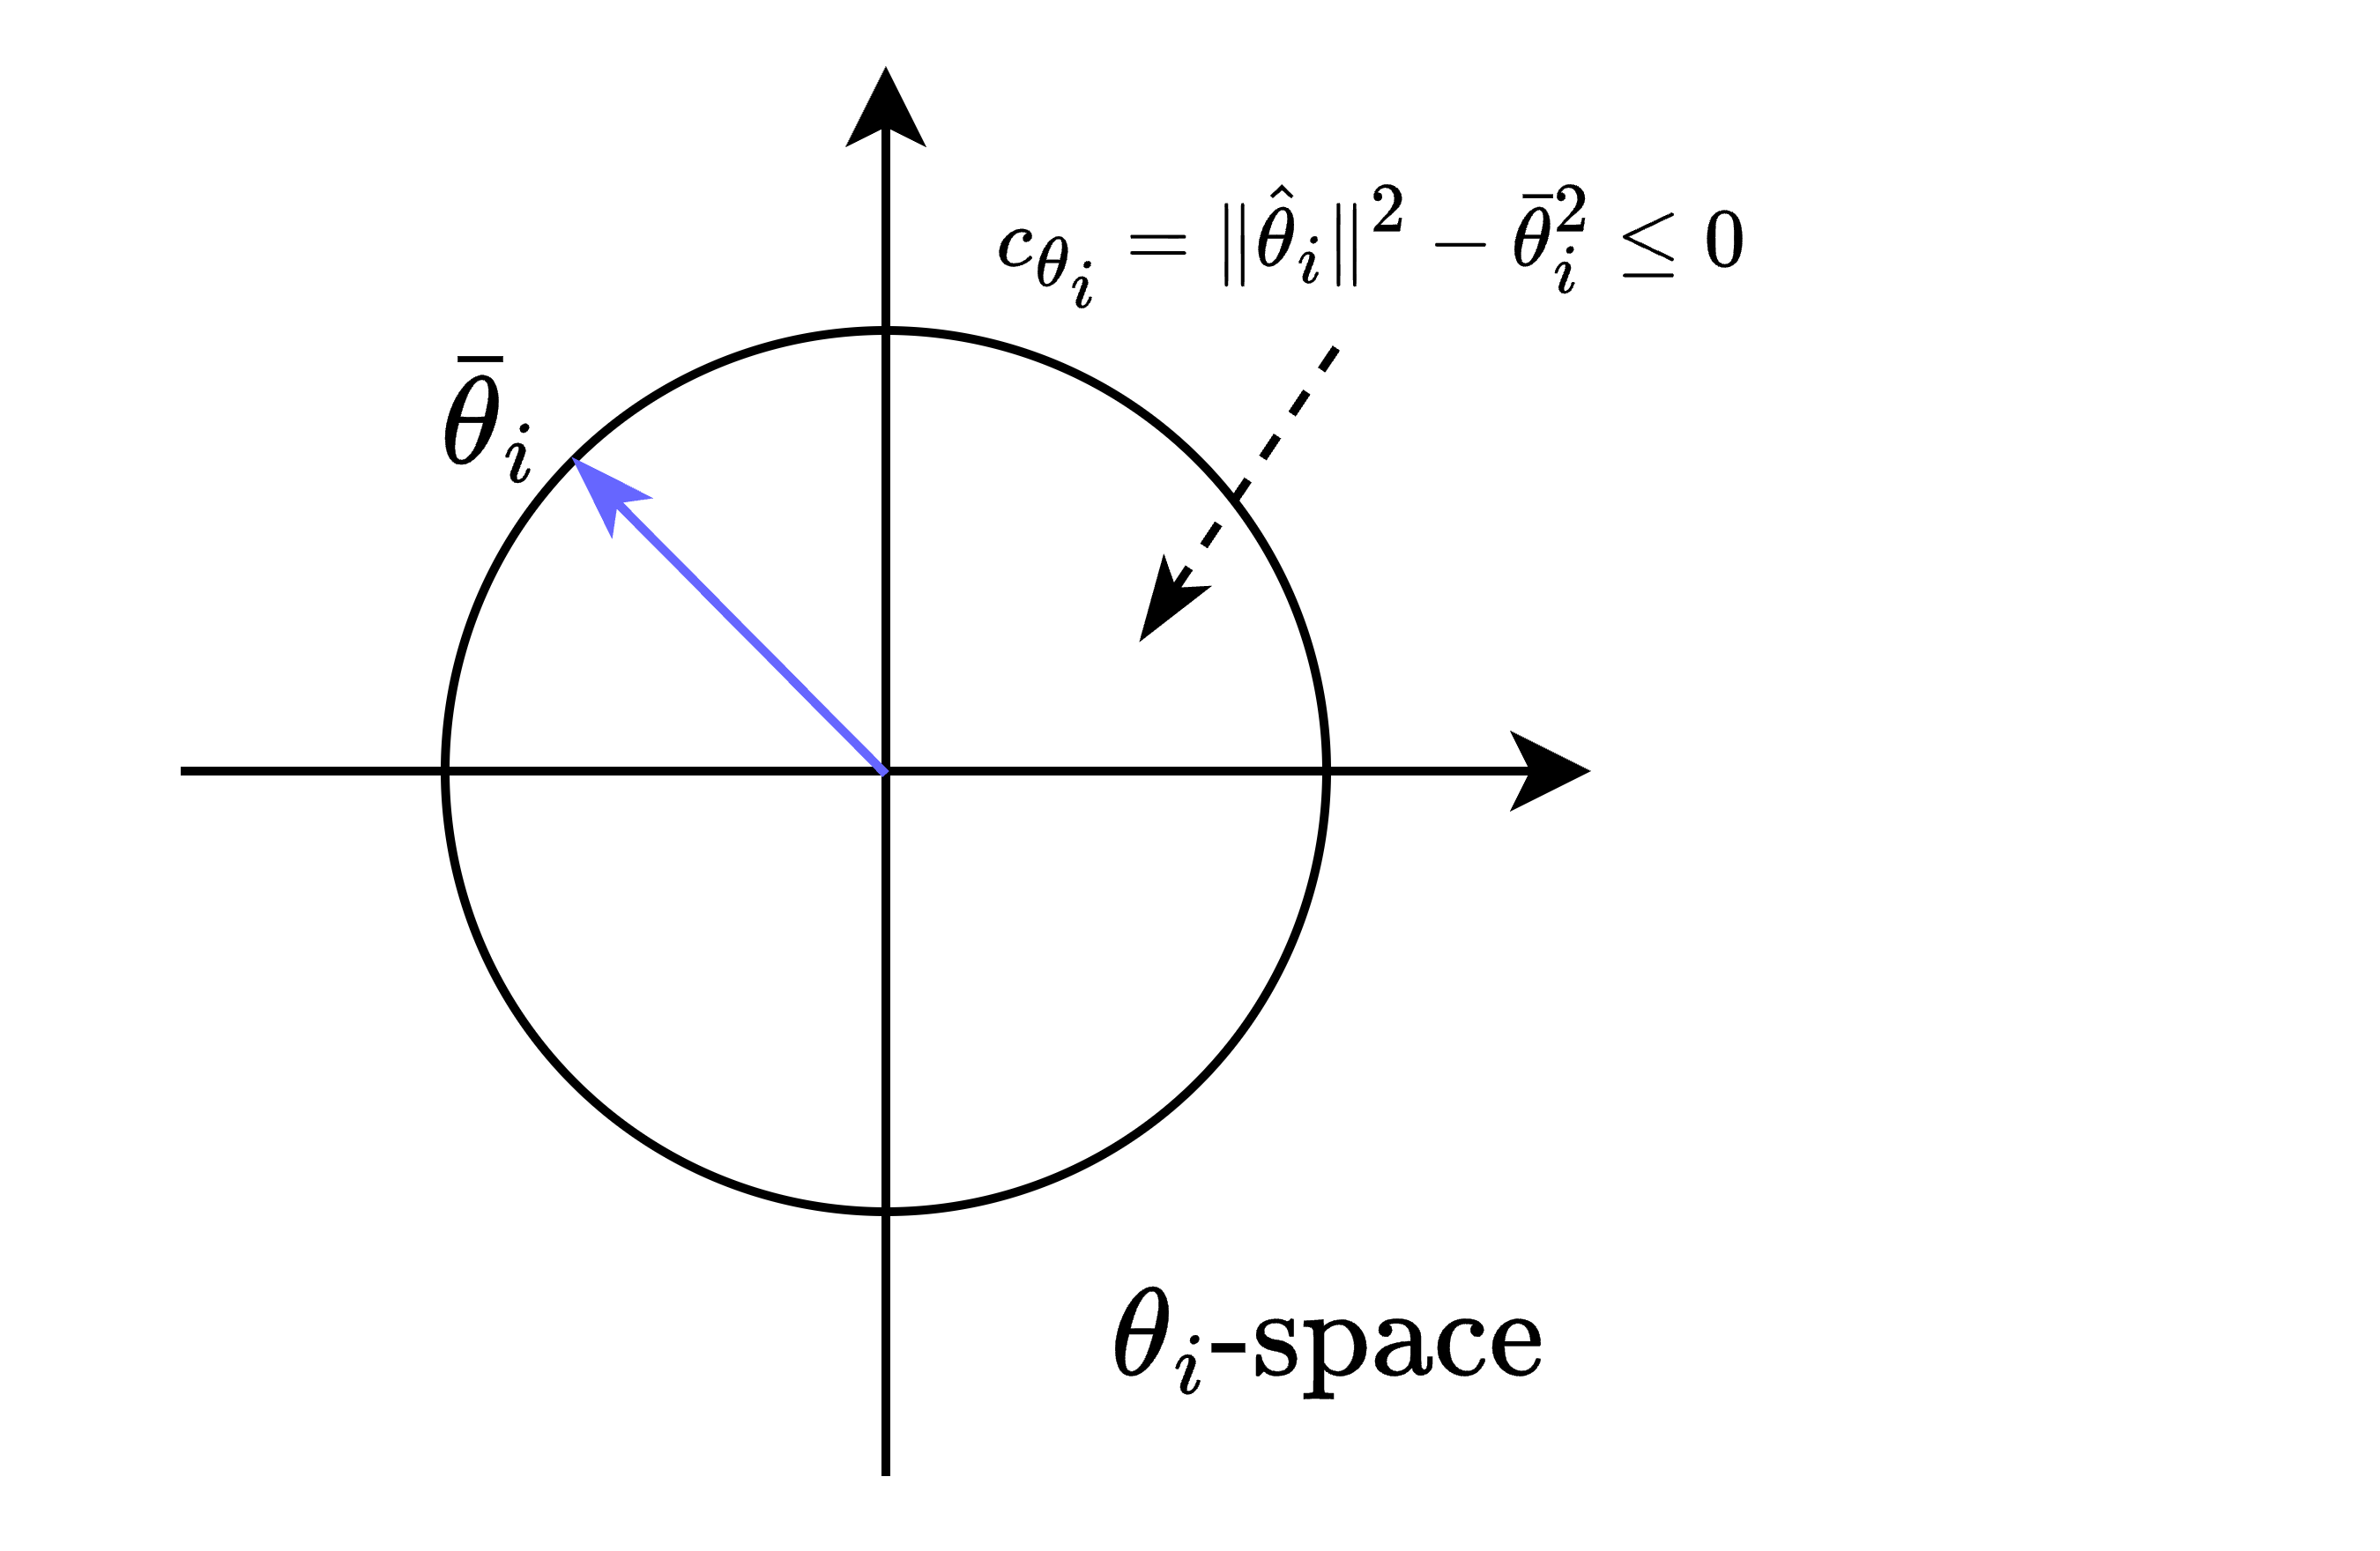
\includegraphics[width=0.5\linewidth]{imgs/cstr_weight.drawio.png}
    \caption{Weight norm constraints.}
    \label{chap4:fig:cstr:weight}
\end{figure*}

The weight norm constraint $\mathbf{c}_{\theta}\triangleq [c_{\theta_i}]_{i\in[0,\cdots ,k]}\in\R^{k+1}$ limits the maximum norm of each layer's weight vector as shown in Fig.~\ref{chap4:fig:cstr:weight}, where
\begin{equation}
    c_{\theta_i}=\Vert \hat\theta_i\Vert^2 -\bar\theta_i^2 \le 0
    \label{chap4:eq:cstr:weight}
\end{equation}
with $\bar\theta_i<\infty$ denoting the maximum allowable norm for $\hat\theta_i$. 
The gradient of $\mathbf{c}_\theta$ with respect to $\hat\theta$ is given by
\begin{equation}
    {\partial \mathbf c_\theta \over \partial \hat\theta}
    \triangleq
    \begin{bmatrix}
        (\partial c_{\theta_0}/\partial \hat\theta)^T
        \\ 
        \vdots 
        \\
        (\partial c_{\theta_k}/\partial \hat\theta)^T
    \end{bmatrix}
    = 2\cdot 
    \begin{bmatrix}
        0&0&\cdots & \hat\theta_0^T\\
        \vdots&\vdots&\ddots&\vdots\\
        0&\hat\theta^T_{k-1}&\cdots &0\\
        \hat\theta^T_k&0&\cdots &0
    \end{bmatrix}
    \in\R^{(k+1)\times\Xi}
    .
    \label{chap4:eq:cstr:weight_grad}
\end{equation}

%\begin{remark} Imposing the weight norm constraint is analogous to applying $L_2$-regularization, a common technique used in DNN training to prevent parameter drift or overfitting \cite{RN23}, by minimizing the $L_2$ norm of the estimated weight vector $\hat\theta$. Typically, $L_2$-regularization adds a term $\lambda\Vert\hat\theta\Vert_2^2$ to the objective function $J$, where $\lambda\in\R_{>0}$ is a constant $L_2$ coefficient. This term biases the trainable weights $\hat\theta$ toward the origin (\ie $\hat\theta = 0$) in the adaptation law \eqref{eq. adaptation law th}. In contrast, within the proposed controller, the term associated with the maximum weight ball constraint in the adaptation law (\ie $\sum_{j\in\mathcal{A}}\lambda_j (\partial c_j/\partial \hat\theta)$ in \eqref{eq. adaptation law th}) vanishes when the constraint is satisfied (\ie $\lambda_j = 0$).
    % 1. 제약조건이 사라져 자유롭게 ball condition 내에서 optimal point로 접근할 수 있다.
%    As a result, $\hat\theta$ can still converge to $\theta^*$ without being restricted to the origin.
%    Moreover, $\lambda_{b_i}$ which corresponds to $\lambda$ varies as the constraint is violated, while $L_2$-regularization has a constant coefficient.
%    \label{remark: ball cstr}
%\end{remark}

\subsection{Input Bound Constraint} \label{chap4:sec:input_cstr}

\begin{figure*}[t]
    \centering
    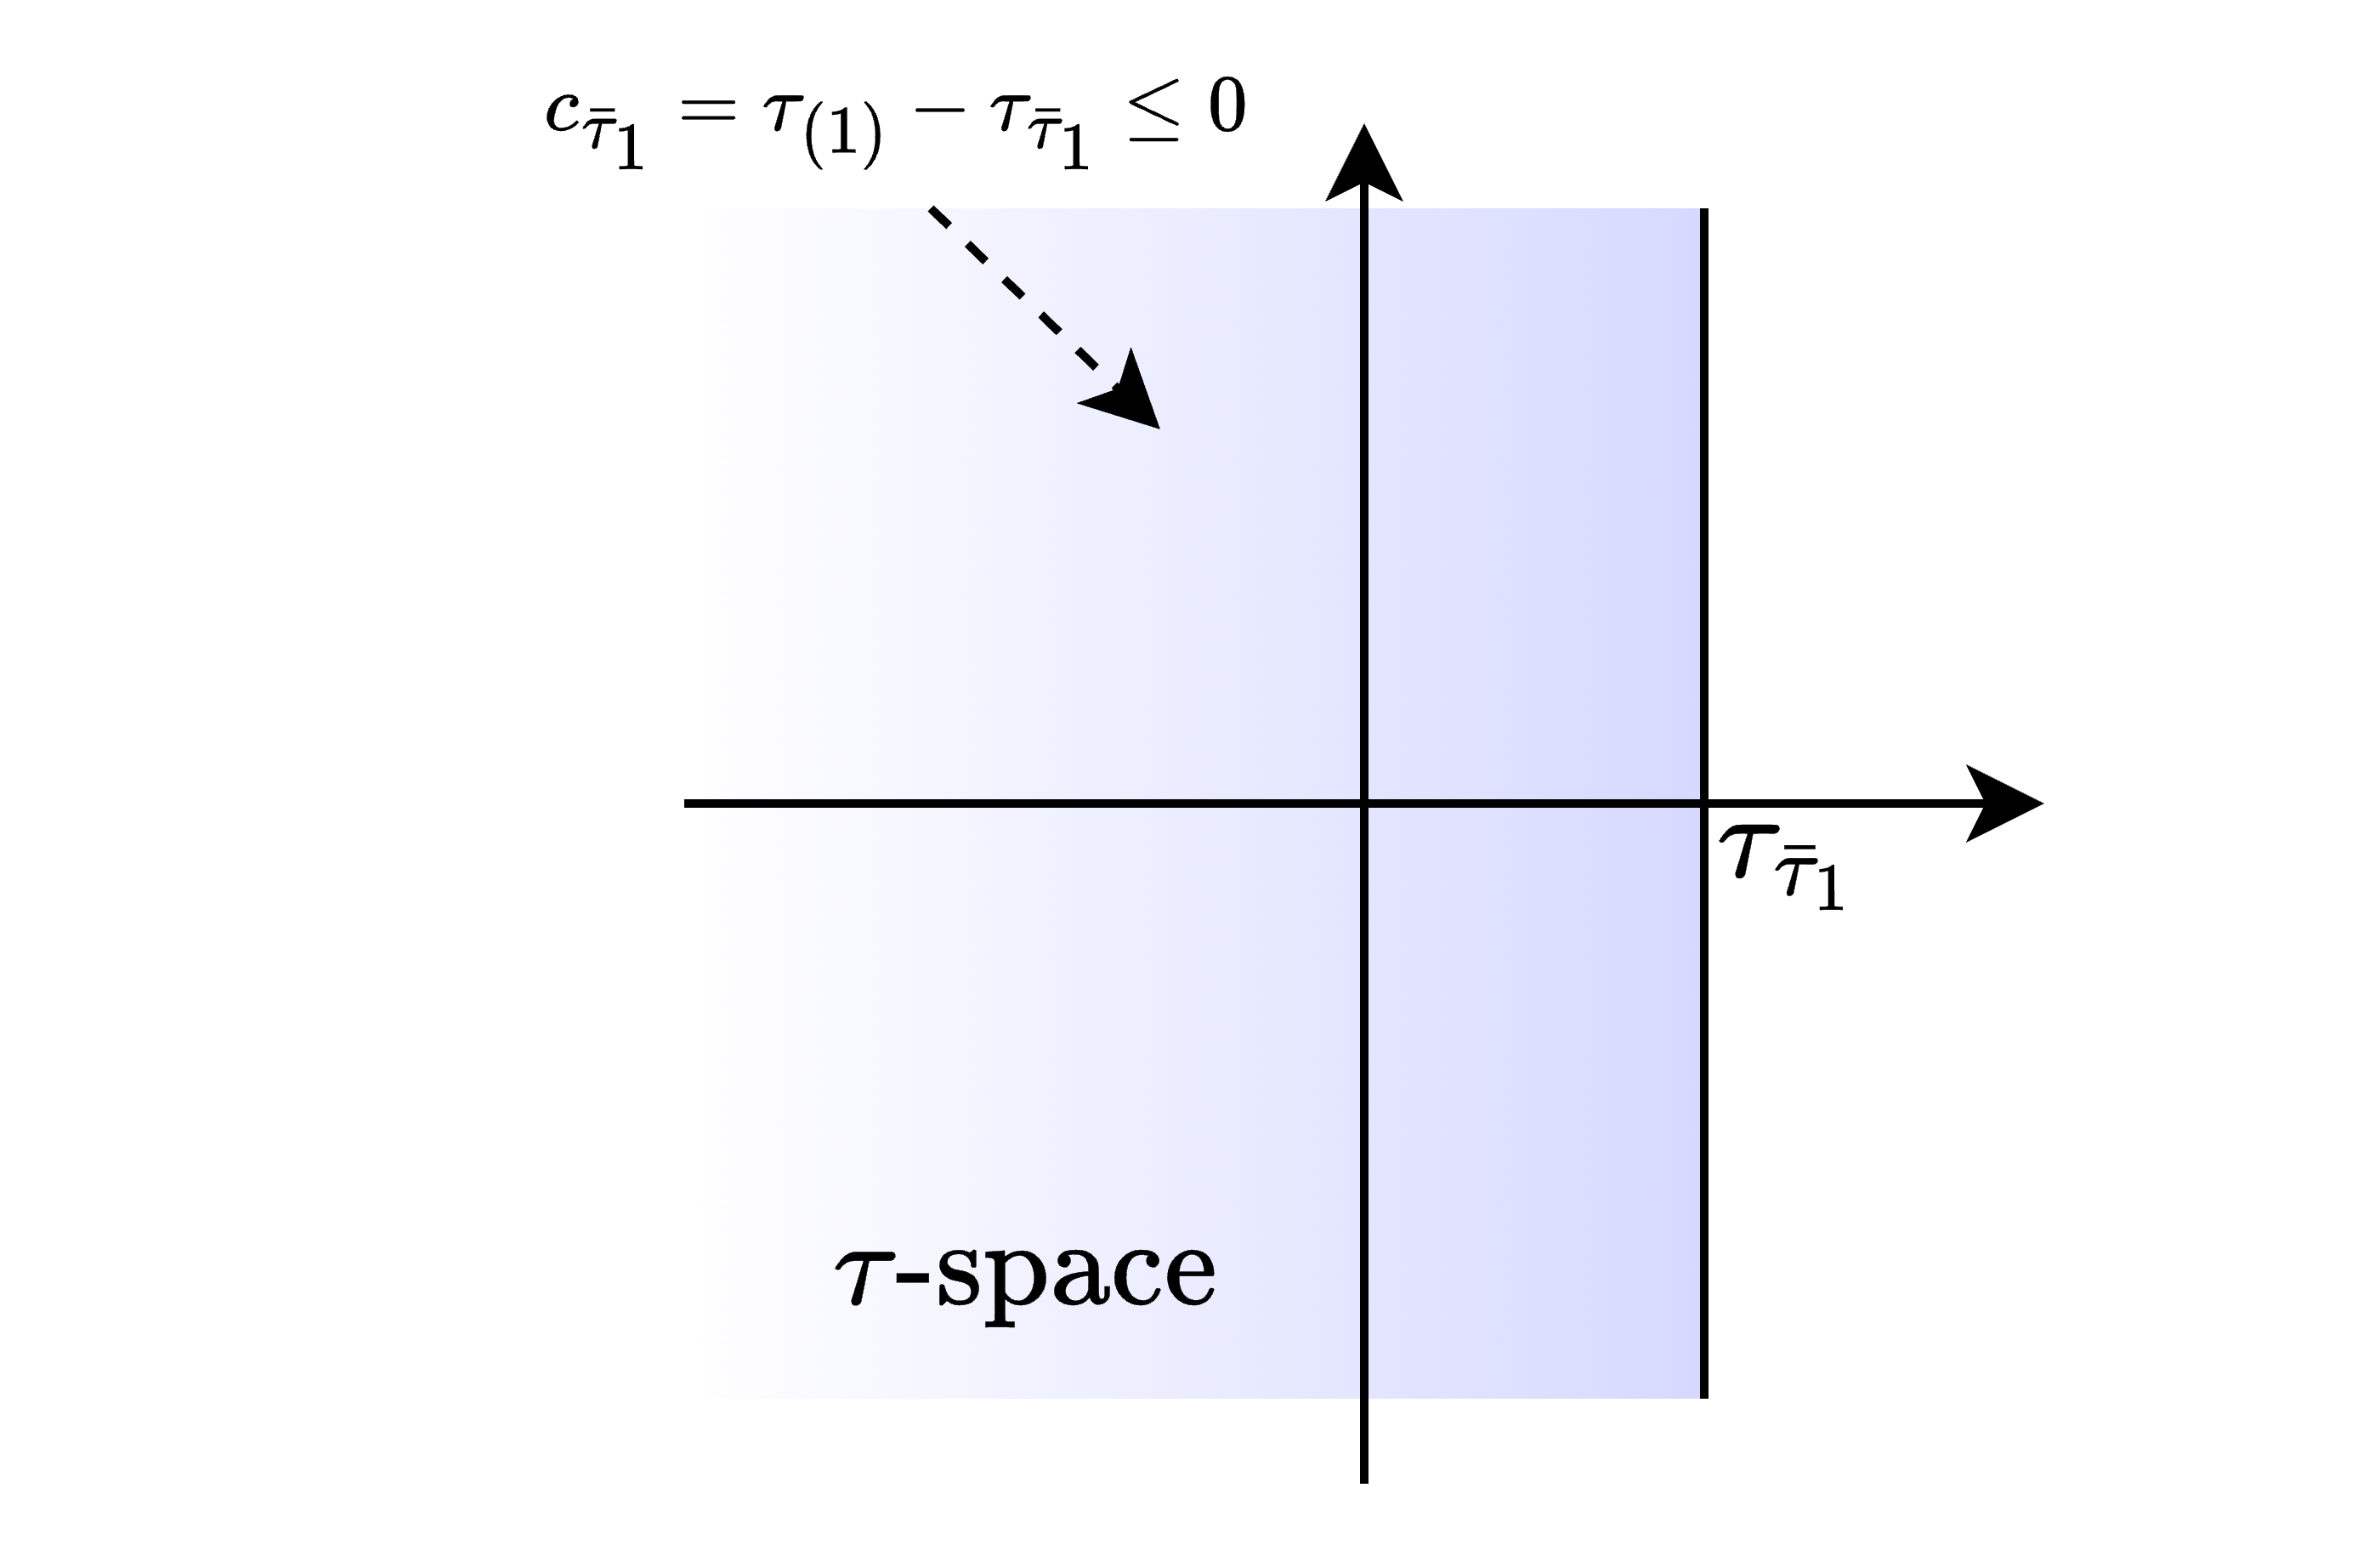
\includegraphics[width=0.5\linewidth]{imgs/cstr_input_bound.drawio.png}
    \caption{Input bound constraints.}
    \label{chap4:fig:cstr:u_bound}
\end{figure*}

Most physical systems have control input limits due to electrical and mechanical limitations. These are expressed as $\mathbf{c}_{\overline \tau}\triangleq [c_{\overline \tau_i}]_{i\in[1,\cdots,n]}$ and $\mathbf{c}_{\underline\tau}\triangleq [c_{\underline\tau_i}]_{i\in[1,\cdots,n]}$, where
\begin{equation}
    \begin{aligned}
        c_{\overline \tau_i}=\tau_{(i)} - {\tau_{\overline \tau_i}} \le 0
        \\
        c_{\underline\tau_i}={\tau_{\underline\tau_i}}-\tau_{(i)} \le 0
    \end{aligned}
    \label{chap4:eq:cstr:input_bound}
\end{equation}
with $\tau_{\overline \tau_i}$ and $\tau_{\underline\tau_i}$ representing the maximum and minimum control input bounds, respectively.
For the case of $c_{\overline{\tau_1}}$ is shown in Fig.~\ref{chap4:eq:cstr:input_bound}.
% The corresponding Lagrange multipliers are $\lambda_{u_j,i},\ \forall j\in[M,m]$. 
The gradients of $\mathbf{c}_{\overline \tau}$ and $\mathbf{c}_{\underline\tau}$ with respect to $\hat\theta$ are given by
\begin{equation}
    \begin{aligned}
        {\partial \mathbf \mathbf c_{\overline \tau} \over \partial \hat\theta}
        \triangleq
        & 
        \begin{bmatrix}
            (\partial c_{\overline \tau_1}/\partial \hat\theta)^T \\
            \vdots \\
            (\partial c_{\overline \tau_n}/\partial \hat\theta)^T
        \end{bmatrix}
         = -{\partial \hat\Phi\over\partial\hat\theta}
        =
        -\begin{bmatrix}
            (I_{l_{k+1}}\otimes \hat\phi_{k}^T)&
            % V_k^T \phi_{k}' (I_{l_{k}}\otimes  \phi_{k-1}^T)&
            \cdots &
            (
            \cdot
            )
        \end{bmatrix} 
        &
        \in
        \R^{n\times \Xi}
        , 
        \\
        {\partial \mathbf \mathbf c_{\underline\tau} \over \partial \hat\theta}         
        \triangleq
        & 
        \begin{bmatrix}
            (\partial c_{\underline\tau_1}/\partial \hat\theta)^T \\
            \vdots \\
            (\partial c_{\underline\tau_n}/\partial \hat\theta)^T
        \end{bmatrix}
        = +{\partial \hat\Phi\over\partial\hat\theta}
        =
        +\begin{bmatrix}
            (I_{l_{k+1}}\otimes \hat\phi_{k}^T)&
            % V_k^T \phi_{k}' (I_{l_{k}}\otimes  \phi_{k-1}^T)&
            \cdots &
            (
            \cdot
            )
        \end{bmatrix} 
        &
        \in
        \R^{n\times \Xi}
        .
    \end{aligned}
    \label{chap4:eq:cstr:input_bound_grad}
\end{equation}

\subsection{Input Norm Constraint} \label{chap4:sec:input_norm_cstr}

\begin{figure*}[t]
    \centering
    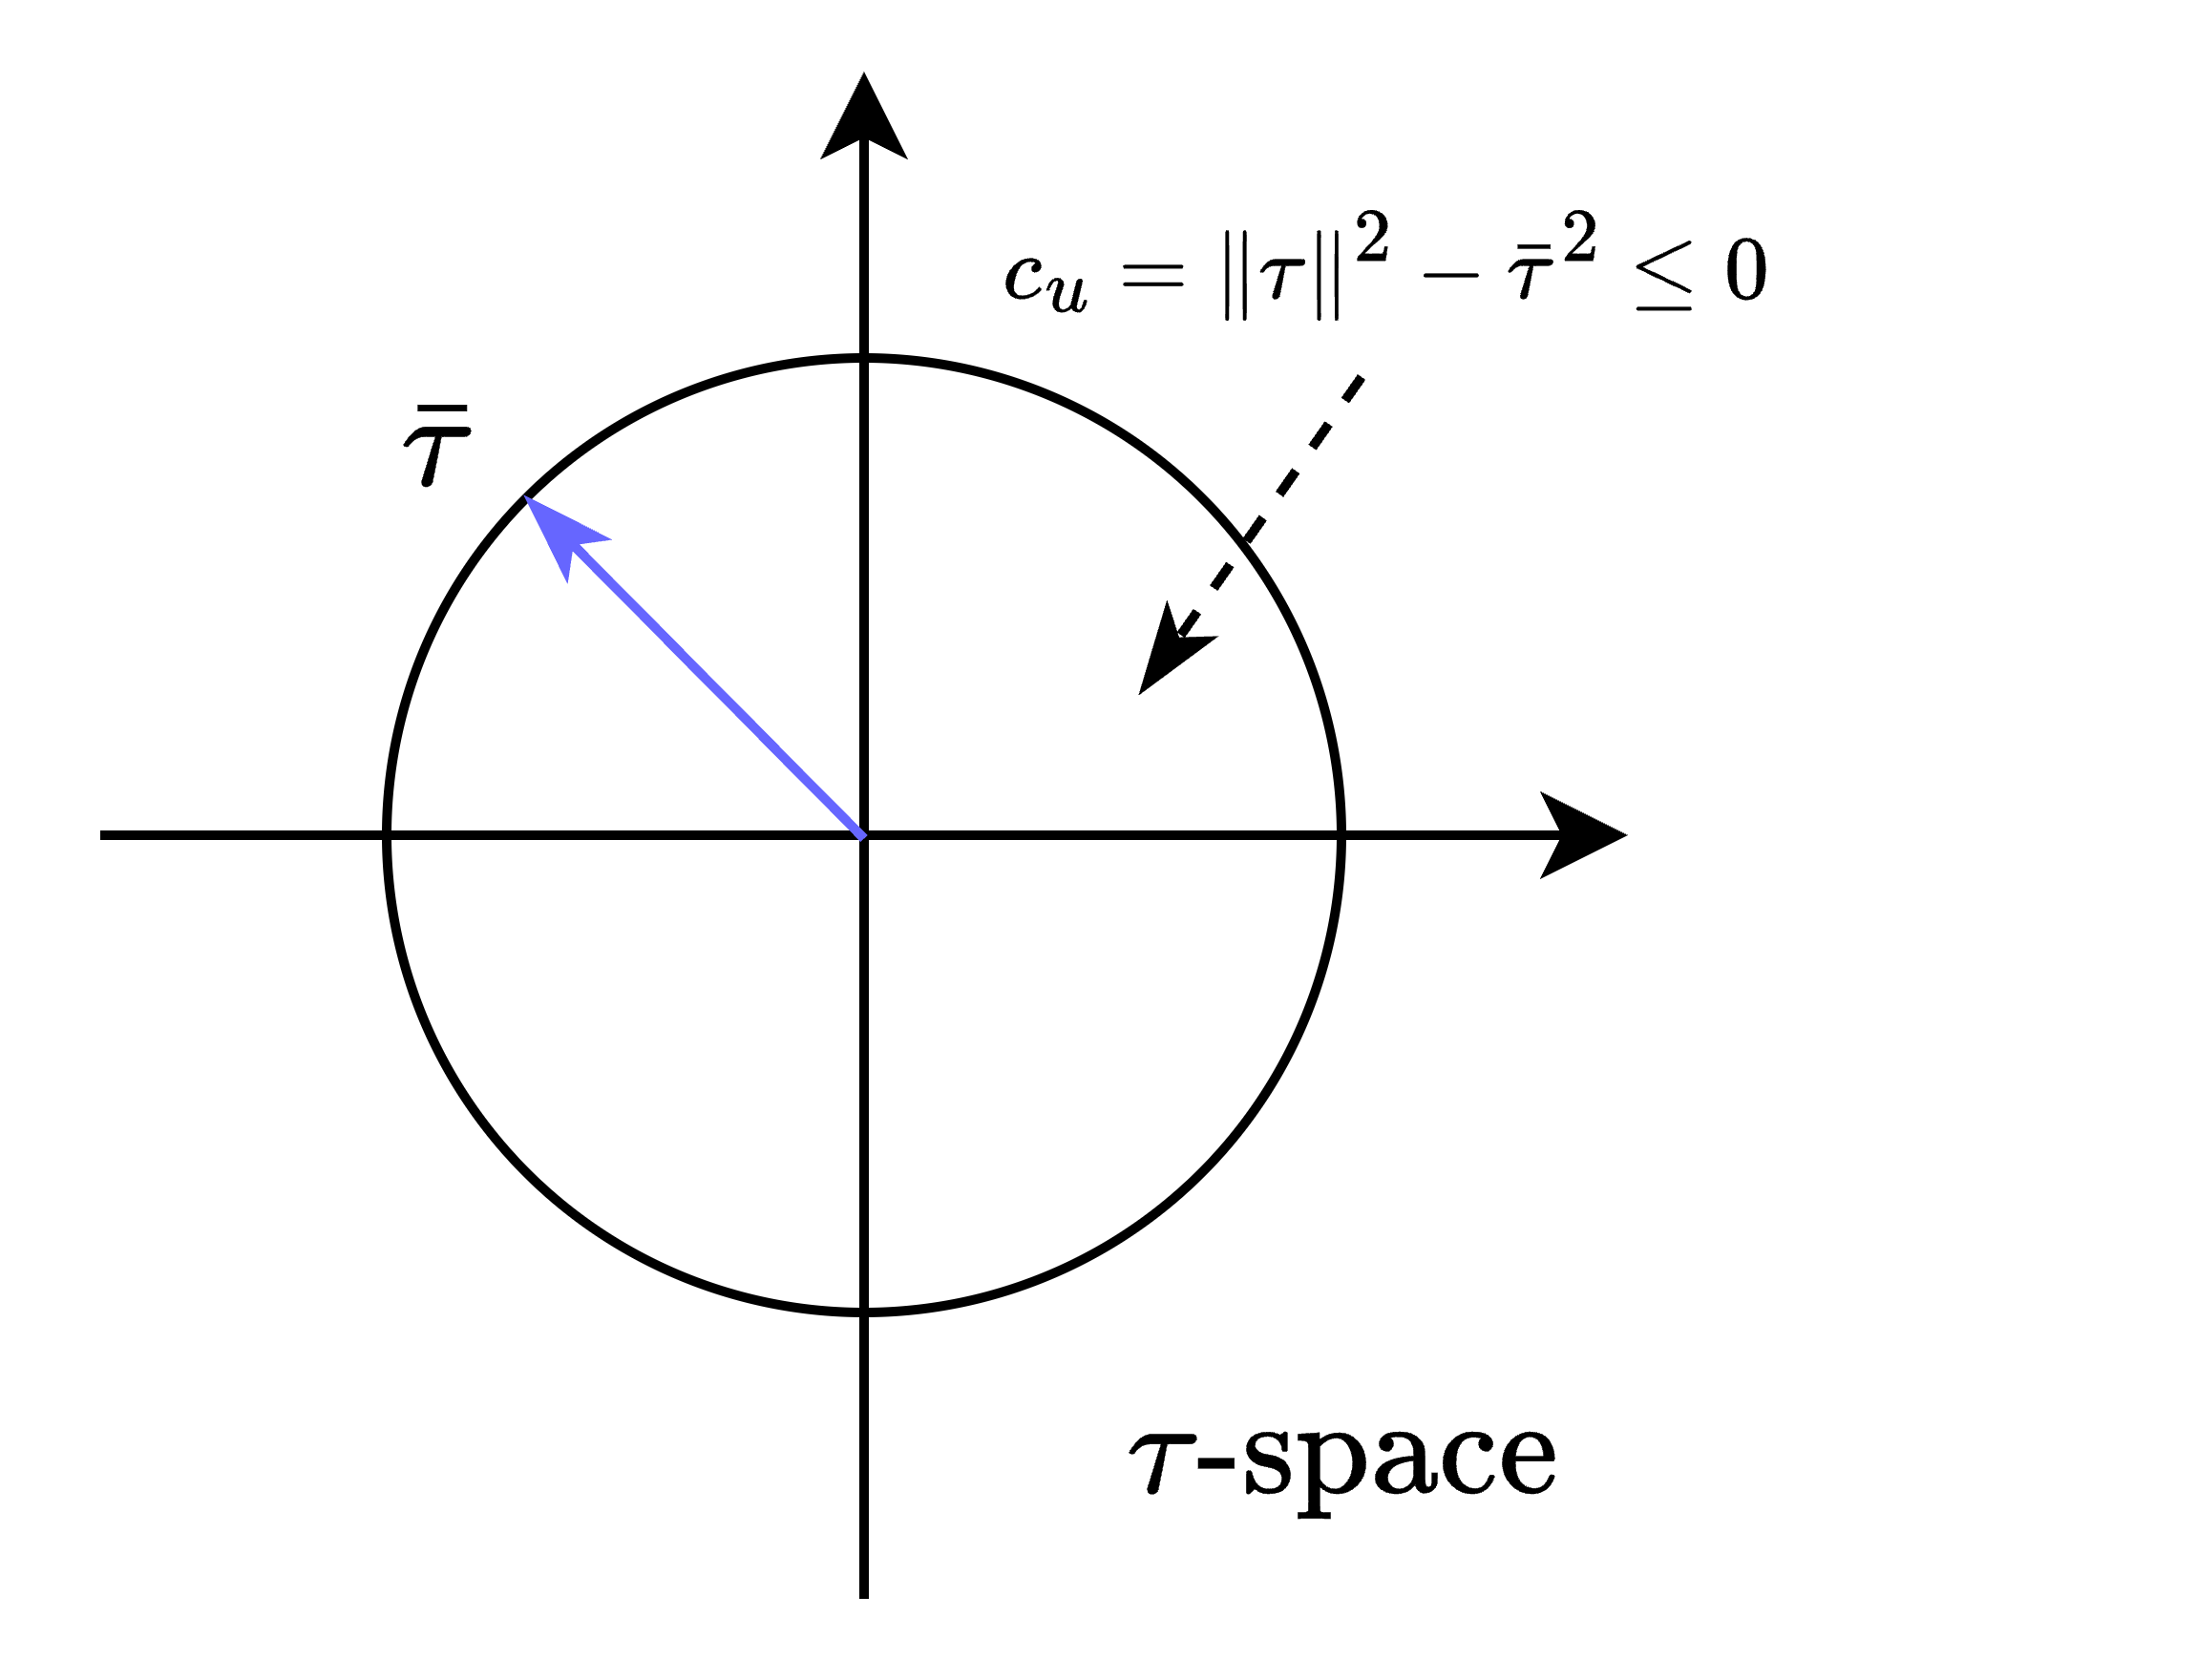
\includegraphics[width=0.5\linewidth]{imgs/cstr_input_norm.drawio.png}
    \caption{Input norm constraints.}
    \label{chap4:fig:cstr:u_norm}
\end{figure*}

Consider the control input $\tau$ as the torque of each actuator corresponding to its generalized coordinate. Since torque is typically linearly proportional to current, actuators that share a common power source are often subject to total current limitations. This can be captured by the following inequality constraint: 
\begin{equation}
    c_{u}=\Vert\tau\Vert^2 -\bar\tau^2  \le 0
    \label{chap4:eq:cstr:input_norm}
\end{equation}
with $\bar\tau\in\R_{>0}$ denoting the maximum allowable control input magnitude as shown in Fig.~\ref{chap4:fig:cstr:u_norm}. 
This input norm constraint is also commonly applied in current and torque control problems for electric motors \cite{RN90}.
% The corresponding Lagrangian multipier is $\lambda_{u_b}$. 
The gradients of $c_{u}$ with respect to $\hat\theta$ are given by
\begin{equation}
    {\partial \mathbf \mathbf c_{u} \over \partial \hat\theta}
    = -\sum_{i=1}^n 2\tau_{(i)} 
    \bigg(
        \text{row}_i
        \bigg(
            -{\partial \hat\Phi\over\partial\hat\theta}
        \bigg)
    \bigg)^T  
    = \tau^T (I_{l_{k+1}}\otimes \hat\phi_k^T)
    \in \R^{\Xi}.
    \label{chap4:eq:cstr:input_norm_grad}
\end{equation}
It should be noted that constraints \eqref{chap4:eq:cstr:input_bound} and \eqref{chap4:eq:cstr:input_norm} cannot be imposed simultaneously, as their gradients \eqref{chap4:eq:cstr:input_bound_grad} and \eqref{chap4:eq:cstr:input_norm_grad} are linearly dependent, violating the LICQ condition.

%%%%%%%%%%%%%%%%%%%%%%%%%%%%%%%%
\section{Stability Analysis} 
%%%%%%%%%%%%%%%%%%%%%%%%%%%%%%%%

Before conducting the stability analysis, let $\tilde\theta\triangleq [\tilde\theta_i]_{i\in[0,\cdots,k]}$, where $\tilde\theta_i\triangleq\hat\theta_i-\theta^*_i$ represents the weight estimation error. The following Lemmas are introduced for the stability analysis. % of the last layer of the DNN.
\begin{lemma}
    If Assumptions \ref{chap4:assum:assum1} and \ref{chap4:assum:assum2} are satisfied, the angle between $\partial c_j/\partial \hat\theta_k$ and $\hat\theta_k$ is positive when $c_j$ is active set, \ie $(\partial c_j/\partial \hat\theta_k)^T\hat\theta_k>0$.
    \label{chap4:lem:lem1}
\end{lemma}

\begin{figure}[!t]
   \centering
   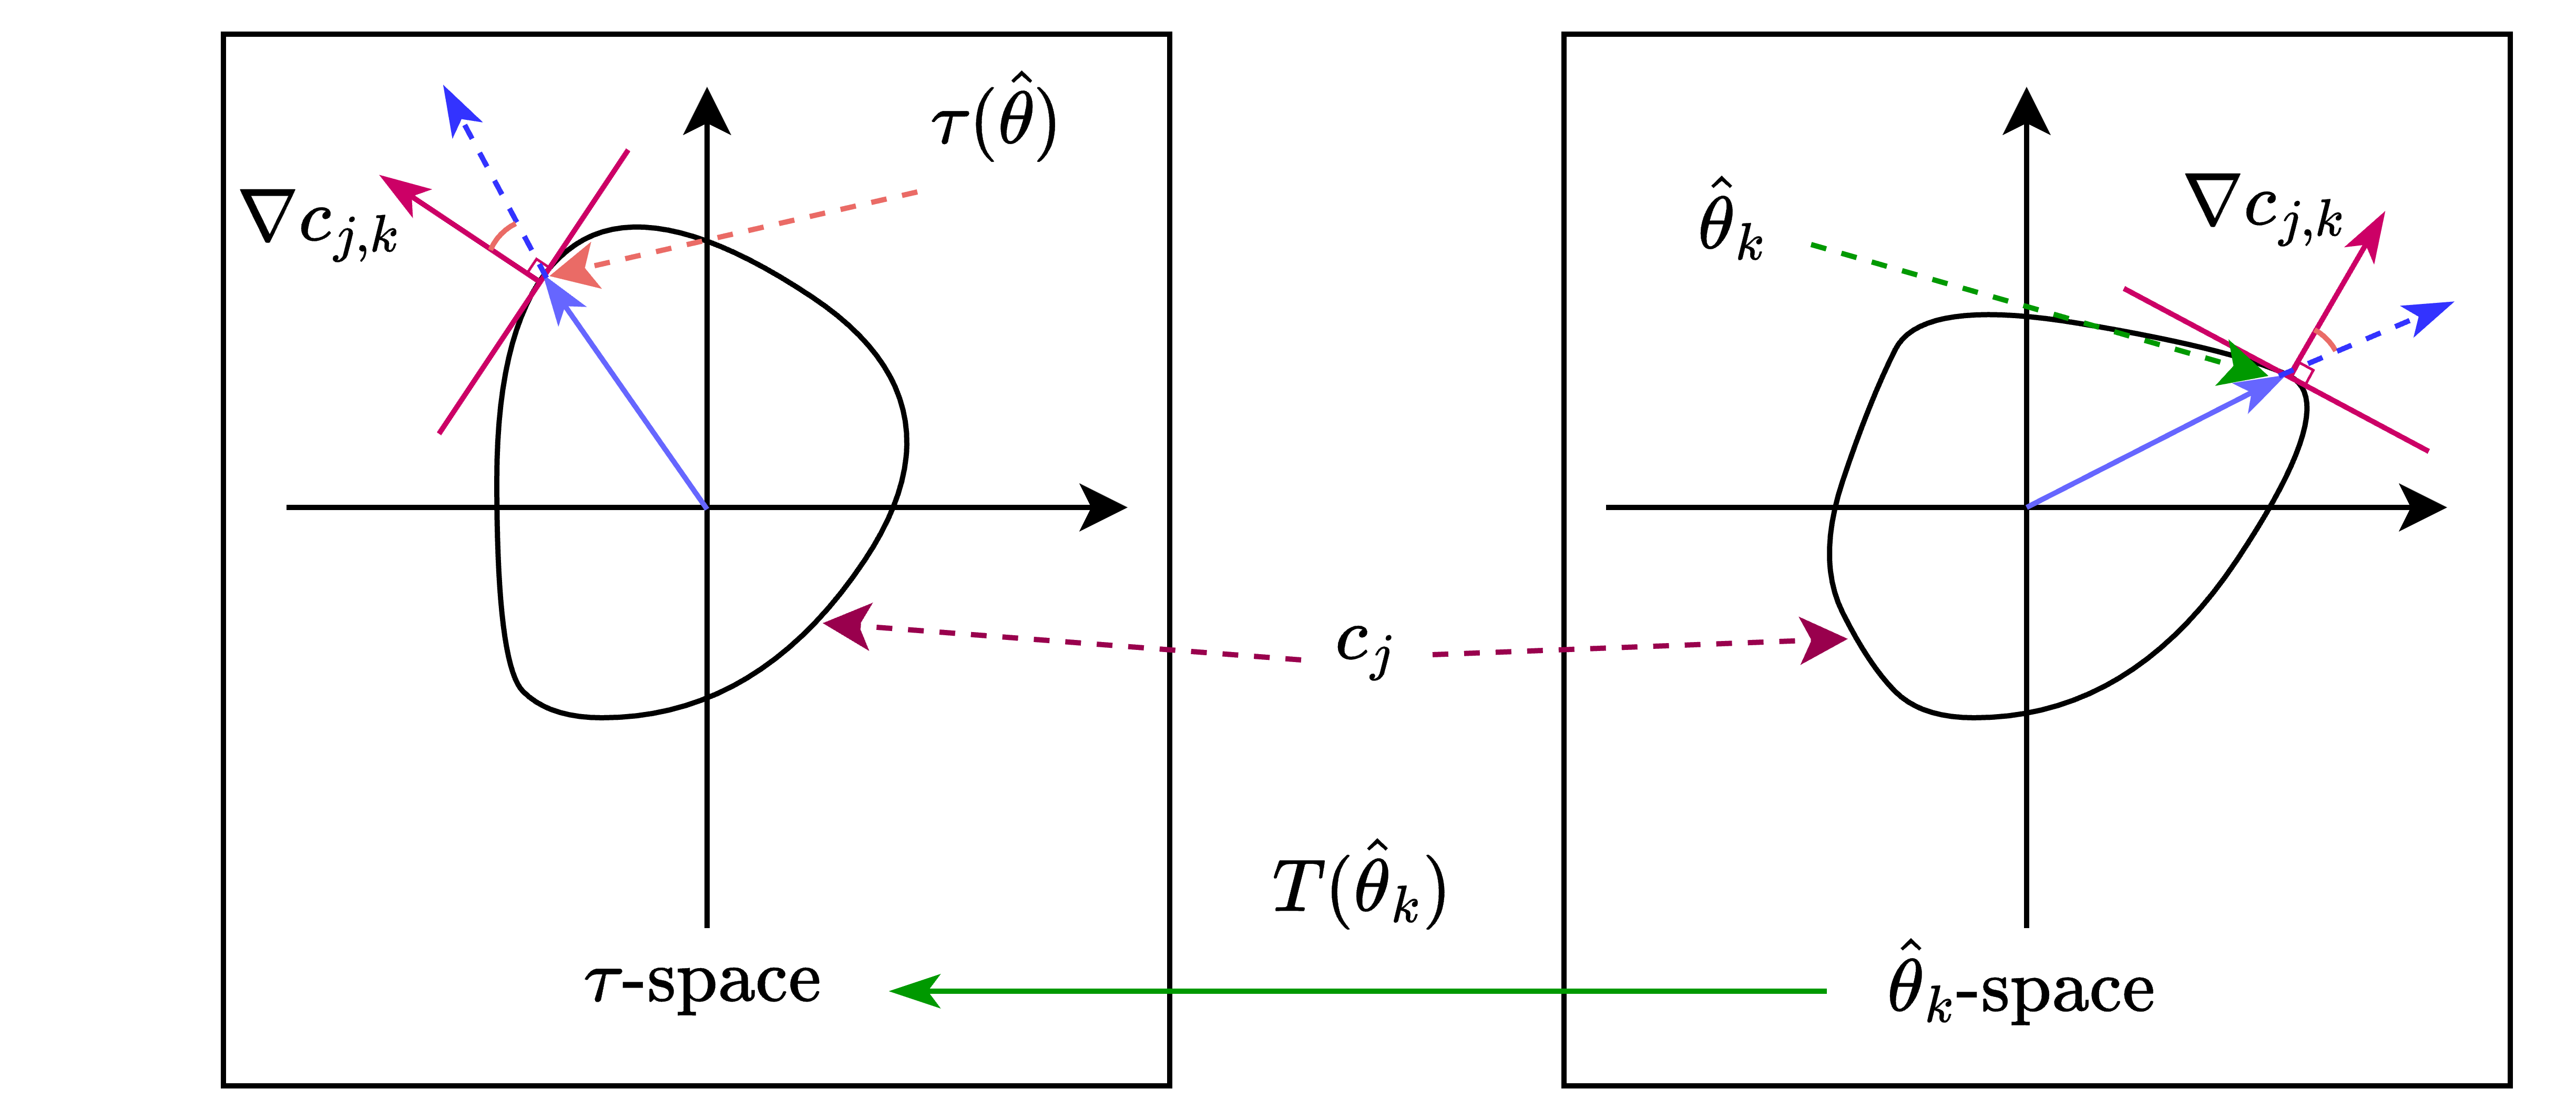
\includegraphics[width=.9\linewidth]{imgs/spaces.drawio.png}
   \caption{Convexity of input constraints.}
   \label{chap4:fig:spaces}
\end{figure}

\begin{proof}

Since $\tau = -\hat\Phi$, using \cite[Proposition 7.1.9]{RN22}, a linear map $T(\cdot):\hat\theta_k\to\tau$ can be derived: 
\begin{equation}
    \begin{aligned}
    \tau = &-\hat\Phi = -\text{vec}(\hat\Phi)     
    = -\text{vec}(\hat V_k \hat\phi_k) 
    \\
    = & -(I_{l_{k+1}}\otimes \hat\phi_k^T)\text{vec}(\hat V_k)
    =-(I_{l_{k+1}}\otimes \hat\phi_k^T)\hat\theta_k = T(\hat\phi_k) \hat\theta_k
    .
    \end{aligned}
    \label{chap4:eq:linear map}
\end{equation}
Therefore, the convexity of the input constraints in $\tau$-space (assumed in Assumption \ref{chap4:assum:assum1}) holds in $\hat\theta_k$-space, implying
%, as depicted in Fig.~\ref{fig: spaces}. 
that $(\partial c_j/\partial \hat\theta_k)^T\hat\theta_k>0$.

\end{proof}

\begin{lemma} 
    If $c_j(\hat\theta),\ \forall j\in\mathcal I \setminus \{\theta_i\}_{i\in[0,\cdots,k]}$ satisfies Assumption \ref{chap4:assum:assum1}, then $\Vert\partial c_j/\partial\hat\theta_i\Vert \allowbreak $, for all $i\in[k-1,\cdots, 0]$, is bounded, provided the norms of $\hat\theta_i$, for all $i\in[k,\cdots, i+1]$, remain bounded.
    \label{chap4:lem:lem2}
\end{lemma}

\begin{proof}

The derivative of $c_j,\ \forall j\in\mathcal I \setminus \{\theta_i\}_{i\in[0,\cdots,k]}$, with respect to $\hat\theta_i$ is represented as
\begin{equation}
    {\partial c_j\over\partial \hat\theta_i} = {\partial c_j\over\partial \tau} {\partial \tau\over\partial \hat\Phi} {\partial \hat\Phi\over\partial \hat\theta_i}
\end{equation}
where $\partial \tau/\partial \hat\Phi=-I_n$, which is bounded. From the linear mapping in \eqref{chap4:eq:linear map}, $\tau$ is bounded as long as $\hat\theta_k$ is bounded (by the condition of the lemma), and $\Vert\phi_k(\cdot)\Vert$ is bounded due to the properties of the activation functions. By Assumption \ref{chap4:assum:assum1}, the function $c_j$ is convex. The convex function has a bounded derivative with respect to $\tau$, since $\tau$ is a bounded variable (\ie $\partial c_j/\partial\tau$ is bounded). Furthermore, $\partial \hat\Phi/\partial \hat\theta_i$ is bounded, provided that the norms of $\hat\theta_i,\ \forall i \in[k,\cdots,i+1]$, are bounded. This can be verified by using the definition of $\partial \hat\Phi/\partial\hat\theta_i$ given in \eqref{chap2:eq:DNNgrad}.
Consequently, $\Vert\partial c_j/\partial \hat\theta_i\Vert,\ \forall j\in\mathcal I \setminus \{\theta_i\}_{i\in[0,\cdots,k]}$, is bounded, when $\hat\theta_i,\ \forall i\in [k,\cdots,i+1]$ are bounded.

\end{proof}

The following theorem shows that $\hat\theta$ and $\xi$ are bounded.

\begin{theorem}
    For the dynamical system in \eqref{chap4:eq:sys1}, the neuro-adaptive controller \eqref{chap4:eq:approx_control} and weight adaptation laws \eqref{chap4:eq:adap_th}, \eqref{chap4:eq:adap_L}, and \eqref{chap4:eq:adap_L_max} ensure the boundedness of the augmented error $\xi$ and the weight estimate $\hat \theta$. This holds with the weight norm constraint \eqref{chap4:eq:cstr:weight} and input constraints satisfying Assumption \ref{chap4:assum:assum2} and \ref{chap4:assum:assum2}, provided that the control gains ${k_q}$ and ${k_z}$ satisfy \eqref{chap4:eq:stable_cond}.
\end{theorem}

\begin{proof}

The boundednesses of $\hat\theta$, $\xi$, and $\eta$ are analyzed recursively from the last $k\textsuperscript{th}$ layer to the first layer of $\hat\Phi$. The step-by-step analysis is described as follows.

\subsubsection{
    Step 1: Boundedness of $\hat\theta_k,\eta_k$, and $\xi$
}

The boundedness of $\xi$ follows from \eqref{chap4:eq:xi_dyna}, using Theorem \ref{chap2:thm:BIBO}, since $A_\xi$ is a stable matrix and the term $B_\xi (\Phi^*-h(\hat\Phi)+\epsilon)$ is bounded due to $\Vert B_\xi\Vert_F$, $\Vert V_k^*\Vert_F$, $\Vert \phi(\cdot)\Vert$, $\Vert h(\cdot)\Vert$, and $\Vert\epsilon\Vert <\infty$.

Assume that all constraints are active in $\mathcal A$ without loss of generality. The dynamics of $\eta_k$ and $\hat\theta_k$ can be decomposed from \eqref{chap4:eq:adap_th} and \eqref{chap4:eq:eta_dyna} as 
\begin{equation}
    \begin{aligned}
        \dot\eta_k =
        & 
        A_\xi \eta_k -B_\xi {\partial h\over\partial\tau}{\partial \hat\Phi\over \partial \hat\theta_k}
        =
        A_\xi \eta_k -B_\xi {\partial h\over\partial\tau}(I_{l_{k+1}}\otimes \hat\phi_k^T)\\
        \dot{\hat\theta}_k =
        & -\alpha 
        \bigg[
            \eta_k^TW\xi+
            \sum_{j\in\mathcal{A}}
            \lambda_j{\partial c_j\over\partial \hat\theta_k}
        \bigg]
    \end{aligned} 
\end{equation}
According to Theorem \ref{chap2:thm:BIBO}, $\Vert \eta_k\Vert_F$ is bounded, since $A_\xi$ is a stable matrix and the term $-B_\xi(\partial h/\partial \tau)(I_{l_{k+1}}\otimes\hat\phi_k^T)$ is also bounded.

Let $\mathcal{V}: \R^{2n} \times \R^{\Xi} \to \R_{>0}$ denote the Lyapunov function:
\begin{equation}
    \mathcal{V} = \frac{1}{2} \xi^T P \xi + \frac{1}{2 \alpha} \hat{\theta}_k^T \hat{\theta}_k,
\end{equation}
with the Lyapunov equation $A_\xi^T P + P A_\xi = -Q$, where $A_\xi < 0$, $P = P^T > 0$, and $Q > 0$.
Taking the time derivative of $\mathcal{V}$ yields:
\begin{equation}
    \begin{aligned}
        \dot{\mathcal{V}} 
        &= -\frac{1}{2} \xi^T Q \xi + \xi^T P B (V_k^{*T} \phi_k^* - h(\tau) + \epsilon) \\
        &\quad - \hat{\theta}_k^T \left( \eta_k W \xi + \sum_{j \in \mathcal{A}} \lambda_j \frac{\partial c_j}{\partial \hat{\theta}_k} \right)
    \end{aligned}
\end{equation}
By applying the boundedness of $\Delta \triangleq P B (V_k^{*T} \phi_k^* - h(\tau) + \epsilon)$ and $M \triangleq \eta_k W$, where $\Vert \Delta \Vert \leq \bar{\Delta} < \infty$ and $\Vert M \Vert_F \leq \bar{M} < \infty$, this simplifies to:
\begin{equation}
    \begin{aligned}
        \dot{\mathcal{V}} 
        &\leq \left( -\frac{\lambda_{\text{min}}(Q)}{2} + \frac{\bar{M}}{2} \right) \Vert \xi \Vert^2 + \bar{\Delta} \Vert \xi \Vert \\
        &\quad + \frac{\bar{M}}{2} \Vert \hat{\theta}_k \Vert^2 - \sum_{j \in \mathcal{A}} \lambda_j \hat{\theta}_k^T \frac{\partial c_j}{\partial \hat{\theta}_k}.
    \end{aligned}
    \label{chap4:eq:V1_dot}
\end{equation}

By representing the term $\partial c_{\theta_k}/\partial \hat\theta_k$ in the last inequality as $\partial c_{\theta_k}/\partial \hat\theta_k=2\hat\theta_k$ using the result provided in \eqref{chap4:eq:cstr:weight_grad}, $\dot {\mathcal V}$ can be rewritten as
\begin{equation}
    \begin{aligned}
        \dot {\mathcal V} \le&
        (\cdot) + 
        \bigg(
            -2\lambda _{\theta_k}+{\bar M}/{2}
        \bigg)
        \Vert\hat\theta_k\Vert^2 
        - \underbrace{
        \sum_{j\in\mathcal{A}\setminus \{\theta_i\}_{i\in[0,\cdots,k]}}\lambda_j\hat\theta_k^T{\partial c_j\over\partial \hat\theta_k}
        }_{>0, \text{\;by Lemma} \ref{chap4:lem:lem1} \text{\;and\;} \text{Assumption} \ref{chap4:assum:assum2}}	
        \\
        \le&
        \bigg(
            -{\lambda_\text{min}(Q)}/{2}+{\bar M}/{2}
        \bigg)
        \Vert\xi\Vert^2
        +\bar \Delta \Vert \xi\Vert 
        + 
        \bigg(
            -2\lambda _{\theta_k}+{\bar M}/{2}
        \bigg)
        \Vert\hat\theta_k\Vert^2 
    \end{aligned}
    \label{chap4:eq:V2_dot}
\end{equation}
Define $P=I_2$, leading to $Q = -A_{\xi}^T - A_{\xi}$. Consequently, the minimum eigenvalues ${\lambda_{\text{min}}(Q)}$ is determined by $2\min({k_q},{k_z})$, as follows from the structure of the matrix $A_{\xi}$. From \eqref{chap4:eq:V2_dot}, if the control gains ${k_q}$ and ${k_z}$ are chosen sufficiently large to satisfy the condition:
\begin{equation}
    % -\lambda_\text{min}(Q)/2+M/2<0
    \min({k_q},{k_z})>\bar M/2
    \label{chap4:eq:stable_cond}
\end{equation}
and if the Lagrange multiplier $\lambda_{\theta_k}$ for the weight norm constraint of the $k\textsuperscript{th}$ layer is increased sufficiently, such that
\begin{equation}
    -2\lambda_{\theta_k} +{\bar M/ 2}<0,  
\end{equation}
(as dictated by \eqref{chap4:eq:adap_L} when the corresponding constraint is violated, \ie $c_{\theta_k}=\Vert \hat\theta_k\Vert^2 -\bar\theta_k^2 > 0$), then both $\xi$ and $\hat\theta_k$ will remain bounded within the compact sets $\Theta_\xi$ and $\Theta_{\hat\theta_k}$, defined as
\begin{equation}
    \Theta_\xi = 
    \bigg\{ \xi \ \bigg\vert\ \Vert\xi\Vert \le  
    {2\bar \Delta\over \lambda _\text{min}(Q)-\bar M} 
    \bigg\}
\end{equation}
and
\begin{equation}
    \Theta_{\hat\theta_k} = 
    \{
    \hat\theta_k 
    \ 
    \vert
    \ 
    \Vert
    \hat\theta_k\Vert \le  
    \bar\theta_k
    \}
    .
\end{equation}
The increase of the Lagrange multiplier $\lambda_{\theta_k}$ will halt once $\hat \theta_k$ reaches the compact set $\Theta_{\hat\theta_k}$. Thus, the Lagrange multiplier $\lambda_{\theta_k}$ is bounded.

The boundedness of the Lagrange multipliers $\lambda_j,\ \forall j\in\mathcal A\setminus\{\theta_i\}_{i\in[0,\cdots,k]}$, can be accessed by considering the convexity of the constraints in $\hat\theta_k$-space.
The boundedness of the remaining Lagrange multipliers associated with the weight norm constraints, $\lambda_{\theta_r},\ \forall r\in[0,\cdots,k-1]$, will be examined in Step $i$. Based on Assumption \ref{chap4:assum:assum1} and Lemma \ref{chap4:lem:lem1},  
%(\ie the constraint is convex on $\tau$-space and $\hat\theta_k$-space, including the origin), 
the equality constraints $c_j \le 0, \ \forall j\in\mathcal A\setminus \{\theta_i\}_{i\in[0,\cdots,k]}$, for convex sets $\Theta_{c_j}$ in $\hat\theta_k$-space.
Let $\Theta_c\triangleq \cap_{j\in\mathcal A\setminus \{\theta_i\}_{i\in[0,\cdots ,k]}} \Theta_{c_j}$ represent the intersection of these convex sets, which also contains the origin.
If $\lambda_j$ increases sufficiently such that $\dot{\mathcal V} \approx -\sum_{j\in\mathcal A\setminus \{\theta_i\}_{i\in[0,\cdots,k]}}\lambda_j\hat\theta_k^T(\partial c_j/\partial \hat\theta_k)<0$, then ${\mathcal V}$, and consequently $\Vert\hat\theta_k\Vert$, will decrease until $\hat\theta_k$ reaches $\Theta_\xi\cap\Theta_{\hat\theta_k}\cap\Theta_c$. Once $\hat\theta_k$ hits the boundary of $\Theta_c$, the Lagrange multipliers will cease to increase, thus ensuring their boundedness.

\subsubsection{Step i: Boundedness of $\hat\theta_i$ and $\eta_i, \ i\in[k-1,\cdots,0]$}

The boundedness of the Frobenius norm of the gradient $\partial\hat\Phi/\partial \hat\theta_i$ can be obtained from its definition in \eqref{chap2:eq:DNNgrad}. This relies on the fact that the boundedness of $\Vert\hat\theta_i\Vert,\ \forall i\in[k,\cdots,i+1]$, was already shown in the previous step (\ie Step 1 to Step $i+1$) and the activation functions $\hat\phi_i$ and their derivative $\hat\phi_i'$ are bounded.

The dynamics of $\eta_i$ and $\hat\theta_i$ for all $i\in [k-1,\cdots,0]$ are represented as
\begin{equation}
    \dot\eta_i = 
    A_\xi\eta_i -B_\xi {\partial h\over\partial\tau}
    {\partial \hat\Phi\over \partial \hat\theta_i}
\end{equation}
and
\begin{equation}
    \begin{aligned}
        \dot{\hat\theta}_i 
        =&
        -\alpha 
        \bigg[
            \eta_i^TW\xi+2\lambda_{\theta_i} \hat\theta_i
            +
            \sum_{j\in\mathcal{A}\setminus \{\theta_i\}_{i\in[0,\cdots,k]}}\lambda_j{\partial c_j\over\partial \hat\theta_i}
        \bigg].
    \end{aligned}
\end{equation}
According to Theorem \ref{chap2:thm:BIBO}, $\Vert\eta_i\Vert_F$ is bounded because $A_\xi$ is a stable matrix and the terms $\Vert B_\xi\Vert, \Vert(\partial h/\partial \tau)\Vert_F$, and $\Vert\partial \hat\Phi/\partial\hat\theta_i\Vert_F$ are bounded.
When $\lambda_{\theta_i}$ is generated due to a violation of the weight norm constraint, $\hat\theta_i$ remains bounded because the term $-2\alpha\lambda_{\theta_i}$ is stable, and the residual terms $\Vert\eta_iW\xi\Vert$, $\lambda_j$, and $\Vert(\partial c_j/\partial \hat\theta_i)\Vert_F$ for all $j\in\mathcal{A}\setminus \{\theta_i\}_{i\in[0,\cdots,k]}$ are bounded, as demonstrated in Step 1 and by Lemma \ref{chap4:lem:lem2}.
The boundedness of each $\lambda_{\theta_i}$ also can be obtained, assuming that $\lambda_{\theta_i}$ is sufficiently increased regulating $\Vert\theta_i\Vert$ into the origin until $c_{\theta_i}$ is satisfied.

Therefore, starting from the boundedness of $\xi$, $\hat\theta_k$, and $\eta_k$ in the $k\textsuperscript{th}$ layer, the boundednesses of $\hat\theta_i$ and $\eta_i$ for the remaining layers $i\in[0,\cdots,k-1]$ can be established recursively, down to the input layer ($i=0$). Thus, $\hat\theta$, $\xi$, and $\eta$ are bounded because $\hat\theta_i,\eta_i,\ \forall i\in[0,\cdots,k]$ and $\xi$ are bounded. Furthermore, since the estimated weight vector $\hat\theta$ is bounded, the weight estimation error $\tilde\theta$ is also bounded, as $\theta^*$ is bounded according to the universal approximation theorem.

\end{proof}

%%%%%%%%%%%%%%%%%%%%%%%%%%%%%%%%
\section{Simulation Validation} 
%%%%%%%%%%%%%%%%%%%%%%%%%%%%%%%%

\subsection{Setup}

The proposed CoNAC was validated using a two-link manipulator model, as depicted in Fig.~\ref{chap4:fig:plant}, adapted from \cite{RN33}. 
The parameters $q_p,{q_d}_p,\tau_p,m_p,l_p,{l_c}_p,b_p$, and ${f_c}_p$ denote the joint angle, desired joint angle, torque, mass, length, center of mass, viscous coefficient, and friction coefficient, respectively, for link $p\in[1,2]$.
%This model contains terms of gravity and friction in its mechanical system.
%These terms make system functions in \eqref{eq. system dynamics 1} nonlinear.
%and can be considered as the disturbance of the system.
The values of the system model parameters are provided in Table~\ref{chap4:table:plant_param}. The desired trajectory for ${q}=[q_1,q_2]^T$ was defined as
\begin{equation}
    {q_d}(t) = 
    \begin{bmatrix}
        {q_d}_1\\{q_d}_2
    \end{bmatrix}
    =
    \begin{bmatrix}
        +\cos(0.49\pi t) + 1 \\
        -\cos(0.49\pi t) - 1 
    \end{bmatrix}.
\end{equation}
%\color{red}
%Considering the power limitation of the power source for the actuators [], 
The control input saturation function was defined as $h(\tau)\triangleq \tau/\Vert\tau\Vert \cdot \text{SSF}_L^U(\Vert\tau\Vert)$, where smooth saturation function (SSF) was adopted from \cite{RN72} and is given by
\begin{equation}
    \text{SSF}_L^U(\Vert\tau\Vert) = {\Vert\tau\Vert\over (1+(\Vert\tau\Vert/\bar\tau)^p)^{1/p}}.
    \label{chap4:eq:sat_h}
\end{equation}
with $p$ being the smoothing factor. The effect of $p$ and the boundedness of $\Vert\partial h/\partial \tau\Vert_F$ is shown in Fig.~\ref{fig: h func}.
The parameters of the control input saturation function were selected as $p=100$ and $\bar\tau=50$. 

In addition to this physically imposed control input saturation, the input norm constraint \eqref{chap4:eq:cstr:input_norm} was imposed to ensure that the control input $\tau$ stays within the unsaturation region of $h(\tau)$ and to prevent inefficient use of the input. With a sufficiently large value for $p$, the input norm constraint essentially matches the control input saturation function. Note that among the selected controllers given below, only the proposed CoNAC can rigorously handle this input norm constraint.

% **********************************************************
% SYSTEM FIGURE AND TABLE
\begin{figure}[!t]
    \centering
    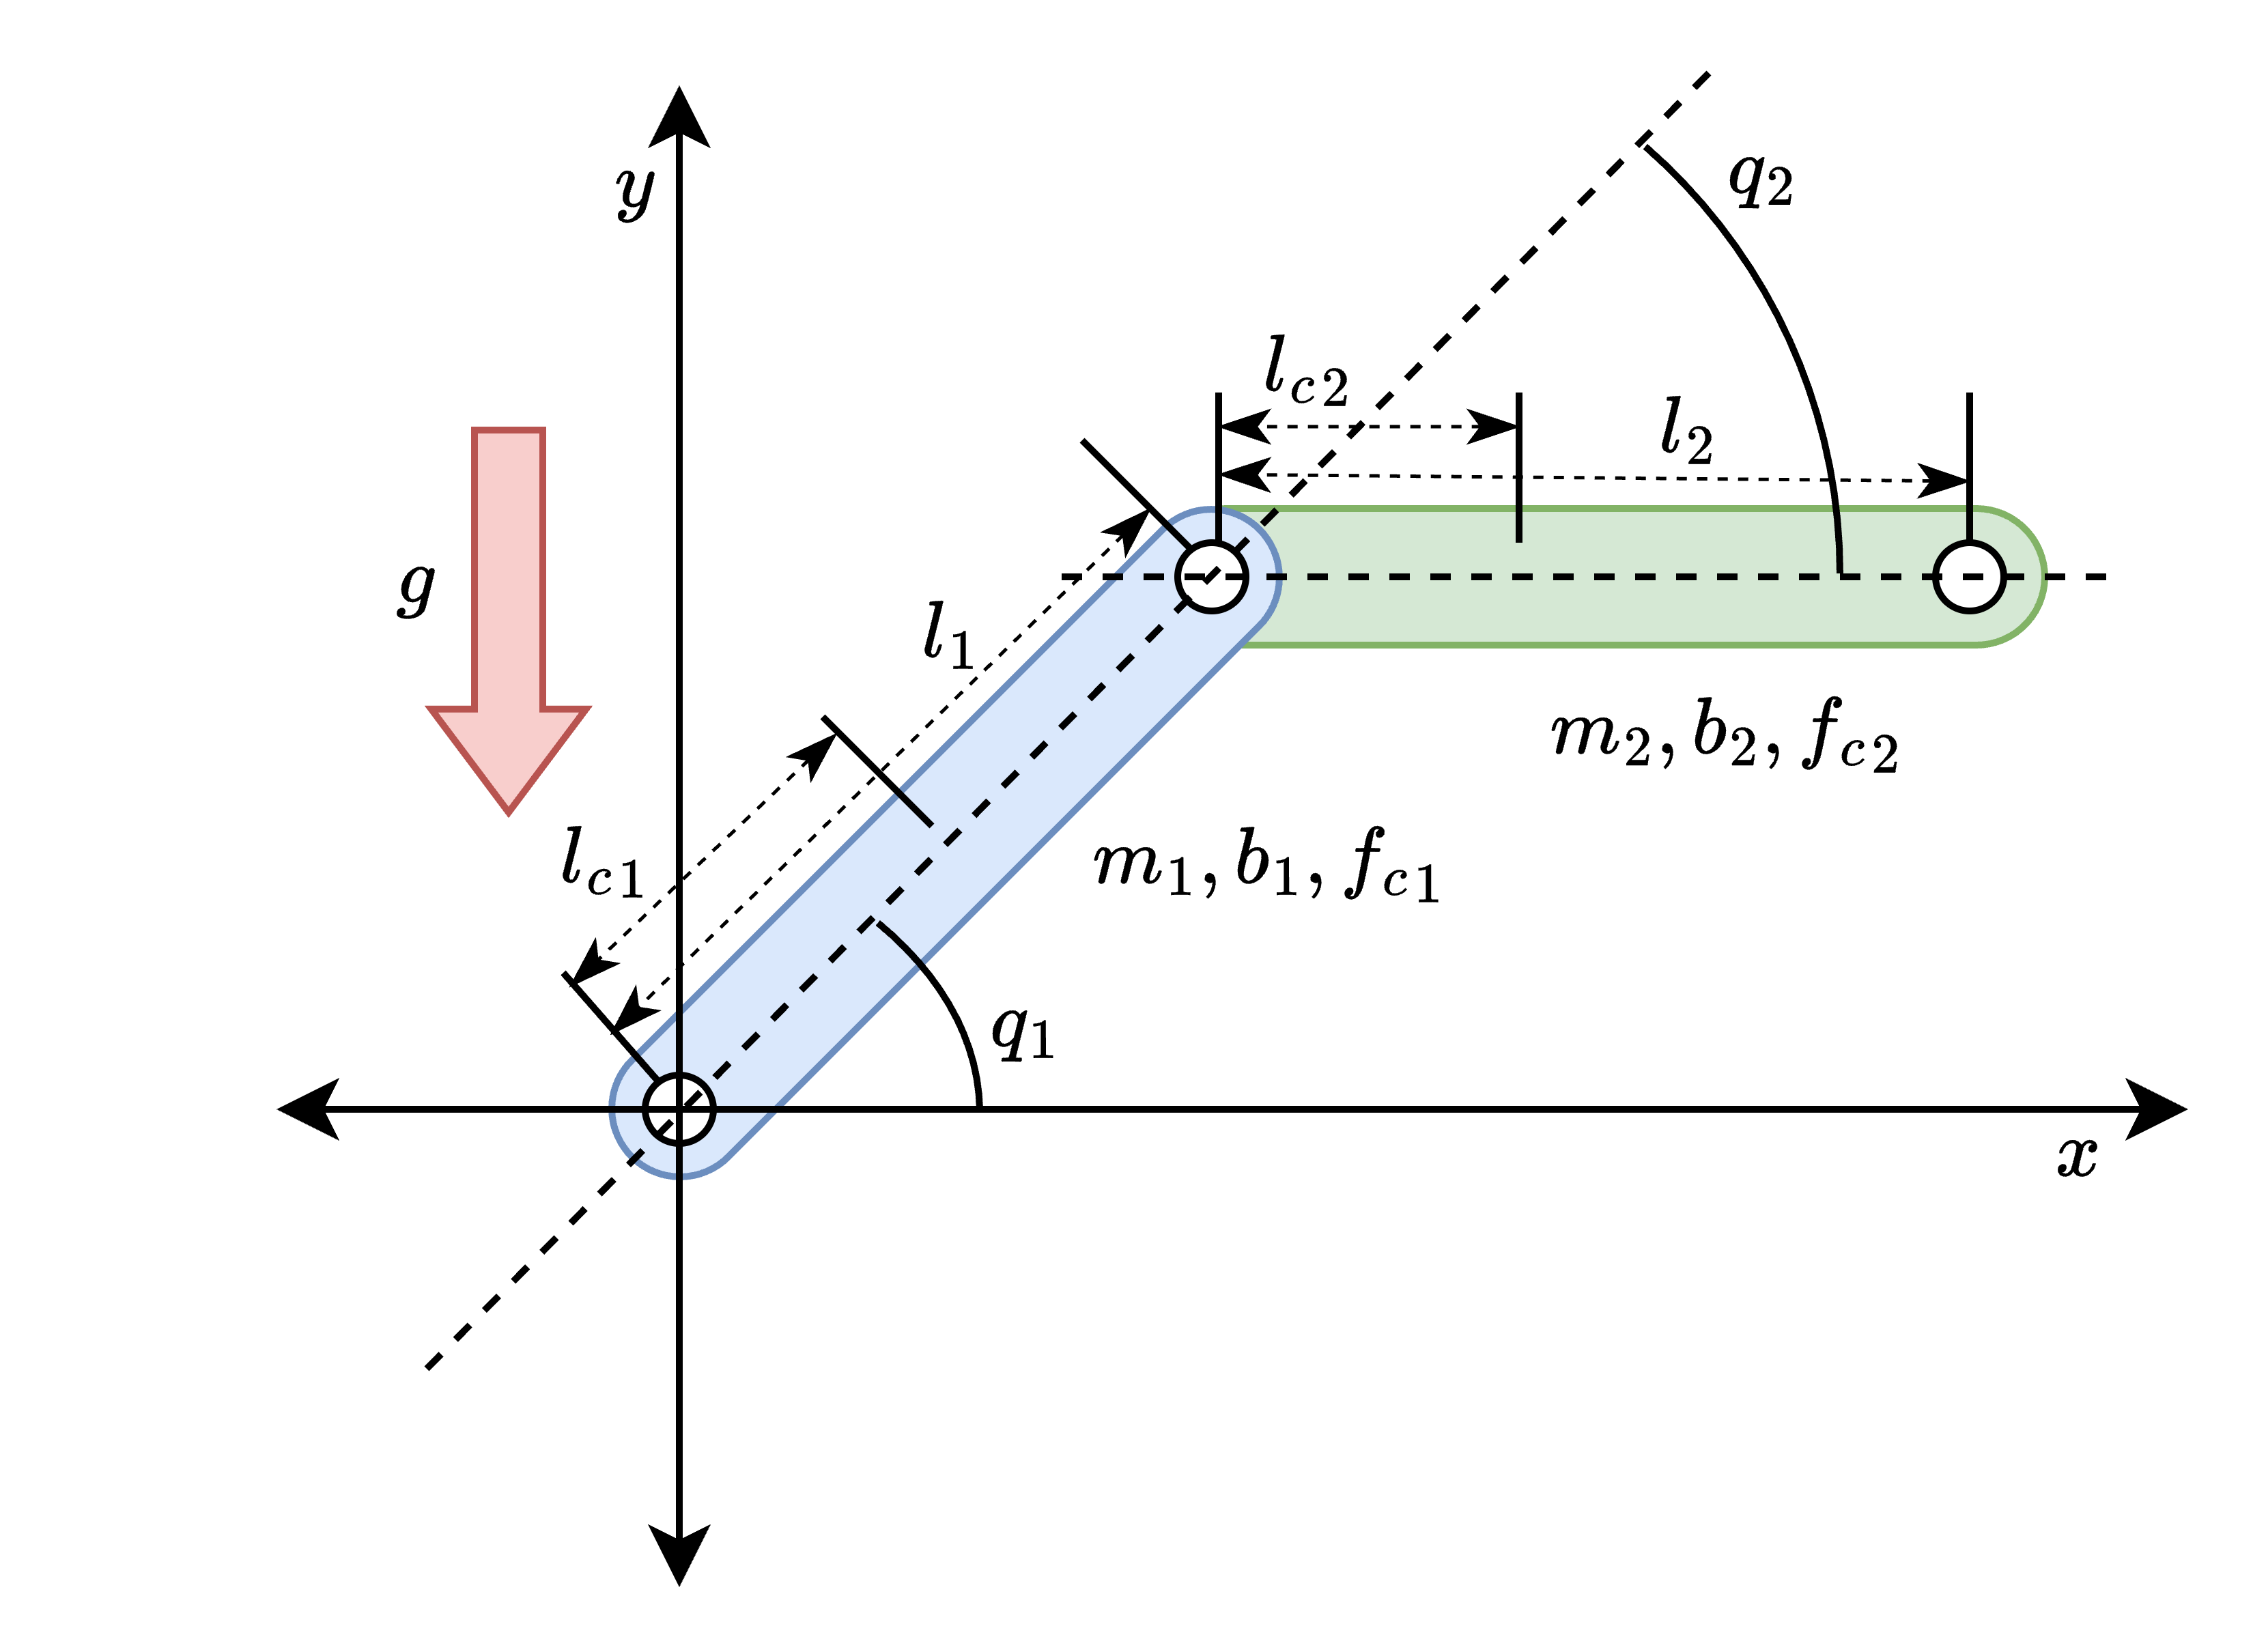
\includegraphics[width=0.7\linewidth]{imgs/RobotModel.drawio.png}
    \caption{Two-link manipulator model.}
    \label{chap4:fig:plant}
\end{figure}

\begin{table}[!t]
    \renewcommand{\arraystretch}{1.3}
    \caption{System model parameters.}
    \centering
    \begin{tabular}{|c||c|c|c|c|}
    \hline
    Symbol & \textbf{Description} & \textbf{Link 1} & \textbf{Link 2} \\
    \hline 
    $m_1, m_2$ & Mass of link    & 23.902 (kg) & 3.88 (kg) \\
    \hline
    $l_1, l_2$  & Length of link   & 0.45 (m) & 0.45 (m) \\
    \hline
    $l_{c1}, l_{c2}$ & COM of link  & 0.091 (m) & 0.048 (m) \\
    \hline
    $b_1, b_2$   & Viscous coefficient  &  2.288 (Nms) & 0.172 (Nms) \\
    \hline
    $f_{c1}, f_{c2}$  & Friction coefficient &  7.17 (Nm) & 1.734 (Nm) \\
    \hline
    \end{tabular}
    \label{chap4:table:plant_param}
\end{table}

\begin{figure}[!t]
    \centering
    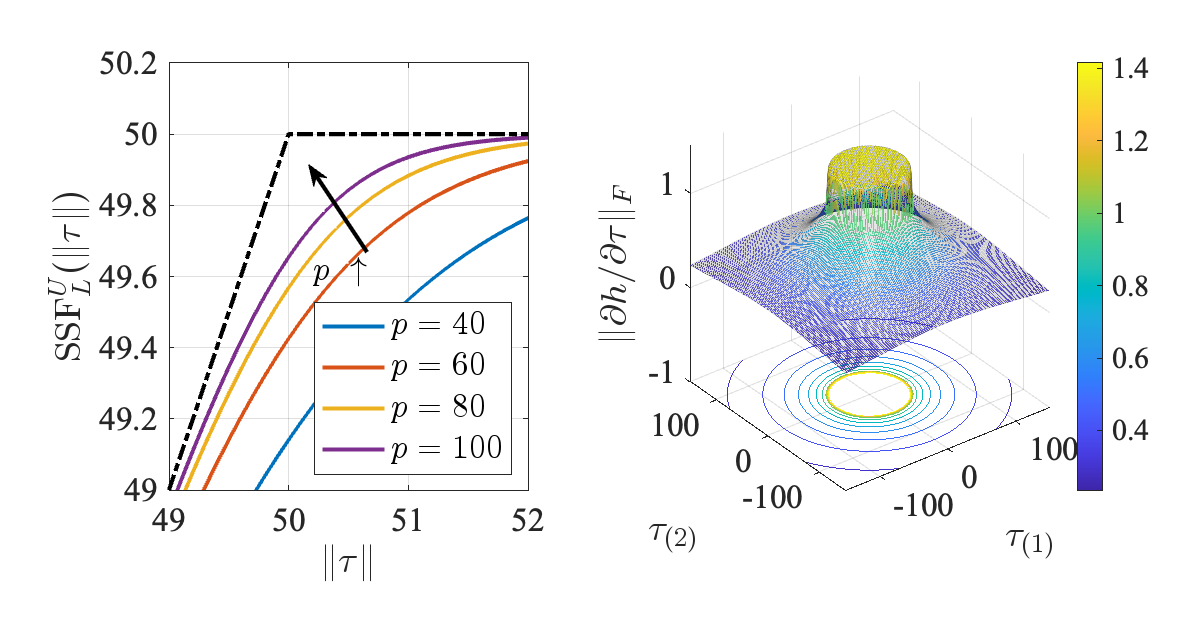
\includegraphics[width=0.85\linewidth]{imgs/Chap4/fig13.eps}
    \caption{Effect of parameter $p$ in the control input saturation function $h$ and boundedness of $\Vert\partial h/\partial \tau\Vert_F$.}
    \label{fig: h func}
\end{figure}

% SYSTEM FIGURE AND TABLE
% **********************************************************
Four controllers were examined for a comparative study. The first was the Backstepping Controller (BSC), used as the baseline. The second was the DNN-based Backstepping Controller (DNN-BSC), an existing neuro-adaptive control method where a DNN was employed to learn and compensate for the lumped system uncertainty function $f$ in the BSC. While this method addressed the weight norm constraint via a projection operator, it did not account for either the input norm or input bound constraints. The third was DNN-BSC augmented with an auxiliary system presented in \cite{RN95,RN46,RN60} (DNN-BSC-A), which handled the (linear) input saturation constraint but not the nonlinear input norm constraint. As a result, an approximation of the input norm constraint was used as an input bound constraint. Lastly, the proposed controller, CoNAC, rigorously considered system uncertainties, the weight norm constraint, and input constraints within a constrained optimization framework. The properties of these four controllers are summarized in Table \ref{chap4:table:ctrl}.

\begin{table}[!t]
    \renewcommand{\arraystretch}{1.3}
    \caption{Properties of the controllers used in simulation}
    \label{chap4:table:ctrl}
    \centering
    \begin{tabular}{|c||c|c|c|}
    \hline
    & \multicolumn{3}{c|}{Handling Capability}\\
    \hline
    & System & Weight Norm & Input Norm\\
    &  Uncertainty & Constraint & Constraint\\
    \hline 
    BSC     & X & X & X\\
    \hline
    \multirow{2}{*}{DNN-BSC}     & \multirow{2}{*}{O} & O & \multirow{2}{*}{X}\\
         &  & (by projection) & \\
    \hline
    \multirow{2}{*}{DNN-BSC-A}   & \multirow{2}{*}{O} & O & $\triangle$ \\
       &  & (by projection) &  (by aux. system)\\
       % &  & & linearized constraint)\\
    % \hline
    % \multirow{3}{*}{DNN-BSC-A}   & \multirow{3}{*}{O} & O & $\triangle$ (by auxiliary\\
    %    &  & (by projection) &  system for \\
    %    &  & & linearized constraint)\\
    \hline
    \multirow{2}{*}{CoNAC}     &  \multirow{2}{*}{O} & O & O\\
         &  & (by optimization) & (by optimization)\\
    \hline
    \end{tabular}
\end{table}

% **** CM1,2 control law *****
The BSC used the control law defined in \eqref{chap4:eq:desired_control} with $\hat f=[0,0]^T$. Since BSC did not consider the unknown system dynamics, the approximation term $\hat f$ was set to zero.
The control law for DNN-BSC was the same as BSC, but the unknown system dynamics were approximated by a DNN \ie $\hat f\approx \hat\Phi$. The adaptation law for DNN-BSC, as presented in \cite{RN13}, was defined by 
\begin{equation}\label{eq:projection}
\dot {\hat\theta}= \text{Proj}_{\Omega}[\alpha  (\partial \hat\Phi/\partial \hat\theta)M_0^{-1}{\tilde z}],
\end{equation}
where $\text{Proj}_{\Omega}(\cdot)$ is the projection operator defined in \eqref{chap3:eq:proj}, which projects an input vector onto a convex set $\Omega$. The convex set was defined as ${\Omega}\triangleq \{\Omega_0\,\cap\,\cdots\,\cap\, \Omega_k\}$, where $\Omega_i\triangleq \{\hat\theta_i\ \vert \ c_{b_i}\le 0\}, \ \forall i\in[0,\cdots, k]$, representing the weight norm constraint \eqref{chap4:eq:cstr:weight}.
% The maximum control input ball constraint is not addressed since the stability analysis of \cite{RN16} uses the property that  $\text{Proj}_\Omega(\cdot)$ projects to the convex set, (\ie the constraints are generally non-convex on the $\hat\theta$-space.).
% **** CM3 control law *****

The control law for DNN-BSC-A was the same as DNN-BSC, but with an auxiliary system to compensate for control input violations. Since the auxiliary system handled only the input bound constraint, not the more complex input norm constraint \eqref{chap4:eq:cstr:input_norm}, an approximated version of the input norm constraint was used as an input bound constraint \eqref{chap4:eq:cstr:input_bound} with ${\overline\tau_i} = -{\underline\tau_i} = (\bar\tau/\sqrt{2}+\bar\tau)/2$. The comparison between the original input norm constraint and its approximation is shown in Fig.~\ref{chap4:fig:control_ball}.
The auxiliary system is defined as $\dot\zeta = A_\zeta \zeta + B_\zeta \Delta\tau,\quad \zeta\vert_{t=0} = 0$, where $\zeta\in\R^n$ denotes the auxiliary state, $A_\zeta=-[20,0;0;20],B_\zeta=[10,0;0,10]$, and $\Delta\tau_{(i)} = 
\tau_{(i)}-\text{sat}(\tau_{(i)},{\overline\tau_i},{\underline\tau_i})$
% s(\tau)-\tau$.
The auxiliary state variables were used in the adaptation law \eqref{eq:projection} by substituting ${\tilde z}$ with ${\tilde z}+\zeta$.

% **** CoNAC control law *****
The proposed CoNAC directly approximated the control law using the DNN as defined in \eqref{chap4:eq:approx_control}. The update rates for the multipliers were set as $\beta_{j}=0.1$. The weight matrix $W$ was selected as $W=\text{diag}([5,1,15,15])]$.

For all DNN-based controllers (DNN-BSC, DNN-BSC-A, and CoNAC), the DNN input vector $q_{NN}$ was set as the desired trajectory for ${q}$, \ie $q_{NN}=[{q_d}^T,1]^T$ with the augmented scalar 1 included to account for the bias term in the weight matrix. 
Each DNN architecture had two hidden layers with eight nodes (\ie $k=2, l_0=2, l_1=8, l_2=8, l_3=2$), and the adaptation gain was set to $\alpha =10^3$. The constraint parameters were $\bar\theta_0=20, \bar\theta_1=30, \bar\theta_2=40$, and $\bar\tau = 50$ (from Eq. \eqref{chap4:eq:sat_h}). The control parameters for all the controllers were set as ${k_q}=1.1,{k_z}=10,M_0=I_2,C_0=I_2,G_0=[0,0]^T$.
The sampling time of the simulations was selected as $T_s=10^{-4}$.

% **********************************************************
% SIMULATION FIGURES
% \begin{figure}[!t]
%     \centering
%         \subfloat[BSC]{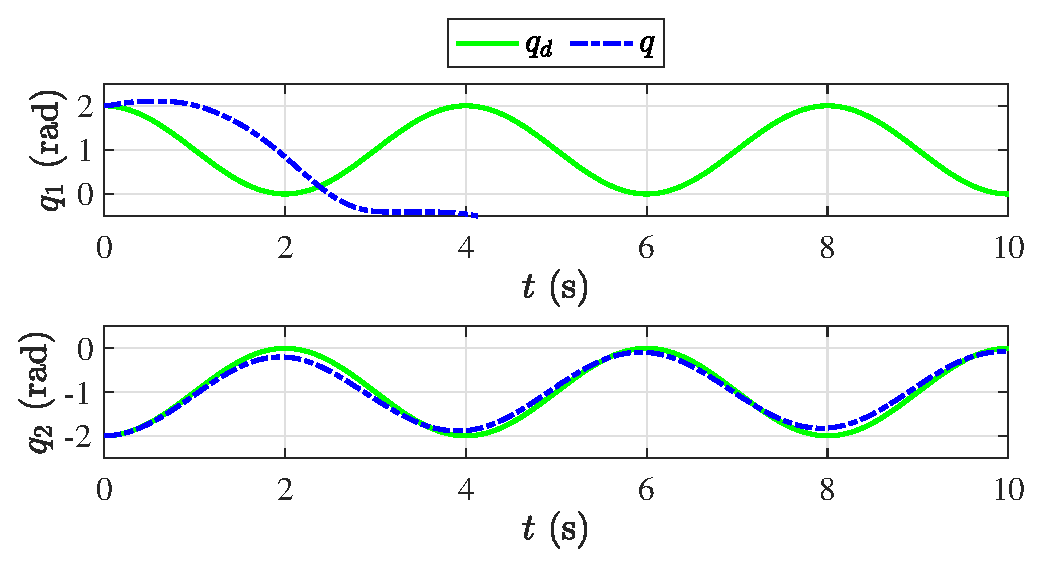
\includegraphics[width=0.49\linewidth]{imgs/Chap4/fig1.eps}%
%         \label{chap4:fig:track_CM1}}
%     \hfill
%         \subfloat[DNN-BSC]{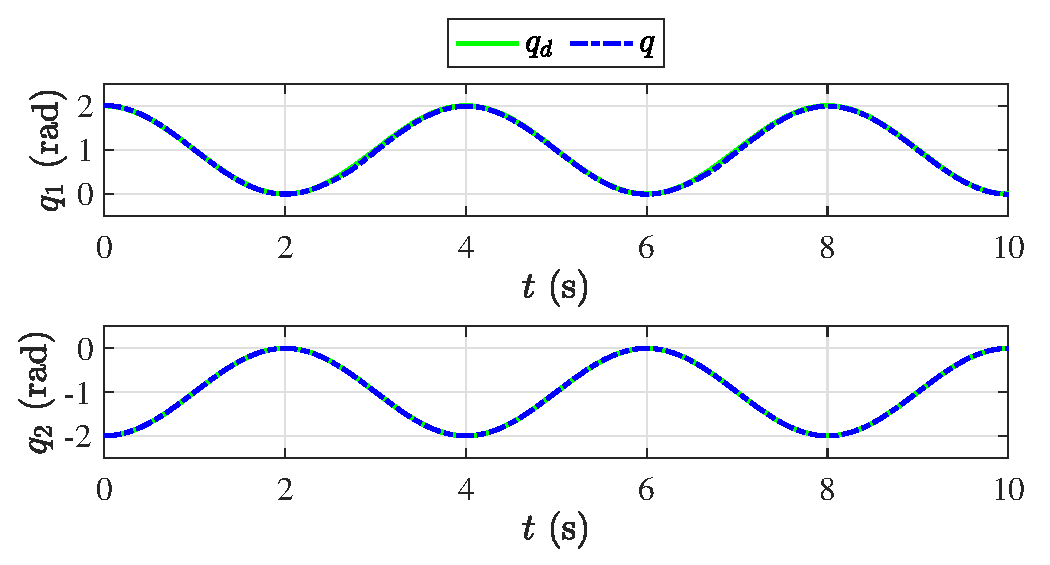
\includegraphics[width=0.49\linewidth]{imgs/Chap4/fig2.eps}%
%         \label{chap4:fig:track_CM2}}
%     \vfill
%         \subfloat[DNN-BSC-A]{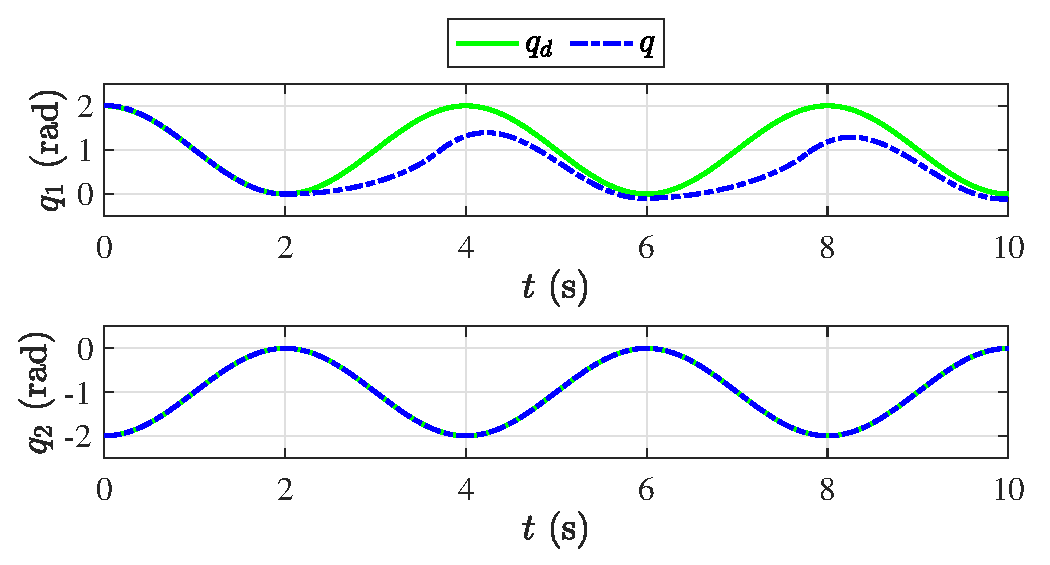
\includegraphics[width=0.49\linewidth]{imgs/Chap4/fig3.eps}%
%         \label{chap4:fig:track_CM3}}
%     \hfill
%         \subfloat[CoNAC]{\includegraphics[width=0.49\linewidth]{imgs/Chap4/fig4.eps}%
%         \label{chap4:fig:track_CoNAC}}
%     \caption{Comparison of the tracking performance across the selected controllers.}
%     \label{chap4:fig:tracking}
% \end{figure}

\begin{figure}[!t]
    \centering
        \subfloat[BSC]{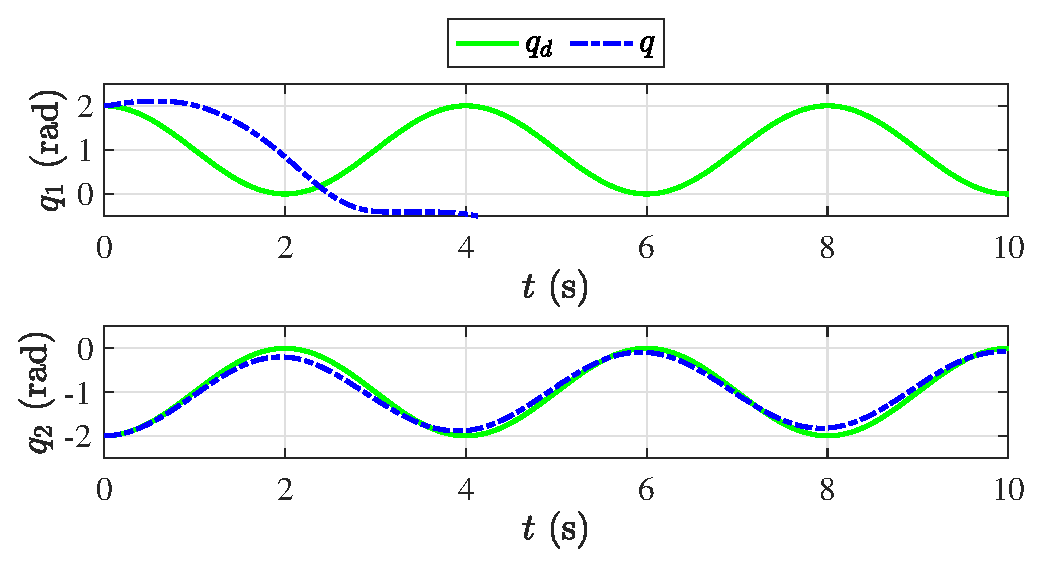
\includegraphics[width=0.8\linewidth]{imgs/Chap4/fig1.eps}%
        \label{chap4:fig:track_CM1}}
    \vfill
        \subfloat[DNN-BSC]{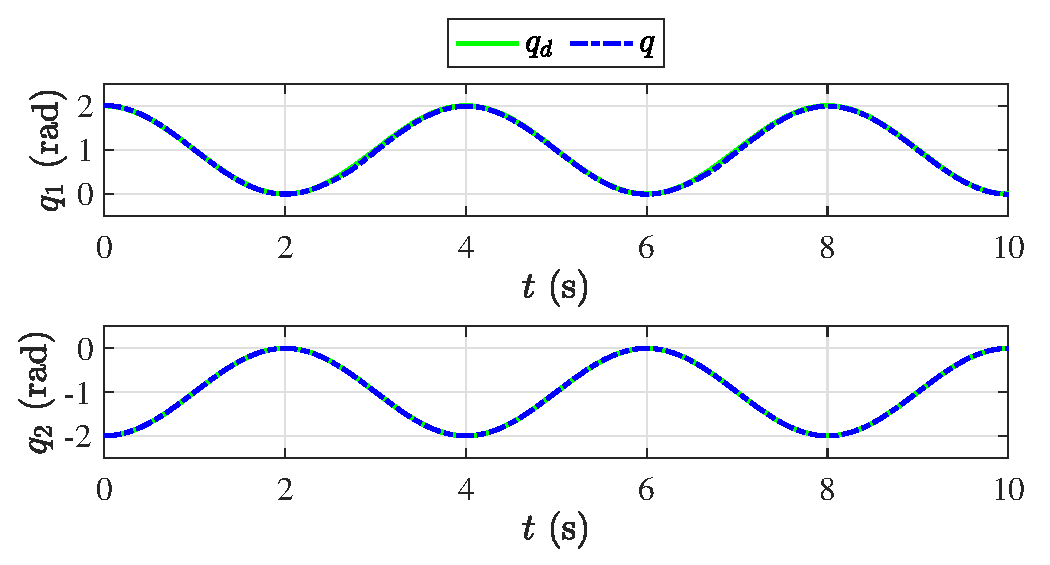
\includegraphics[width=0.8\linewidth]{imgs/Chap4/fig2.eps}%
        \label{chap4:fig:track_CM2}}
    \caption{Comparison of the tracking performance of BSC and DNN-BSC.}
    \label{chap4:fig:tracking1}
\end{figure}

\begin{figure}[!t]
    \centering
        \subfloat[DNN-BSC-A]{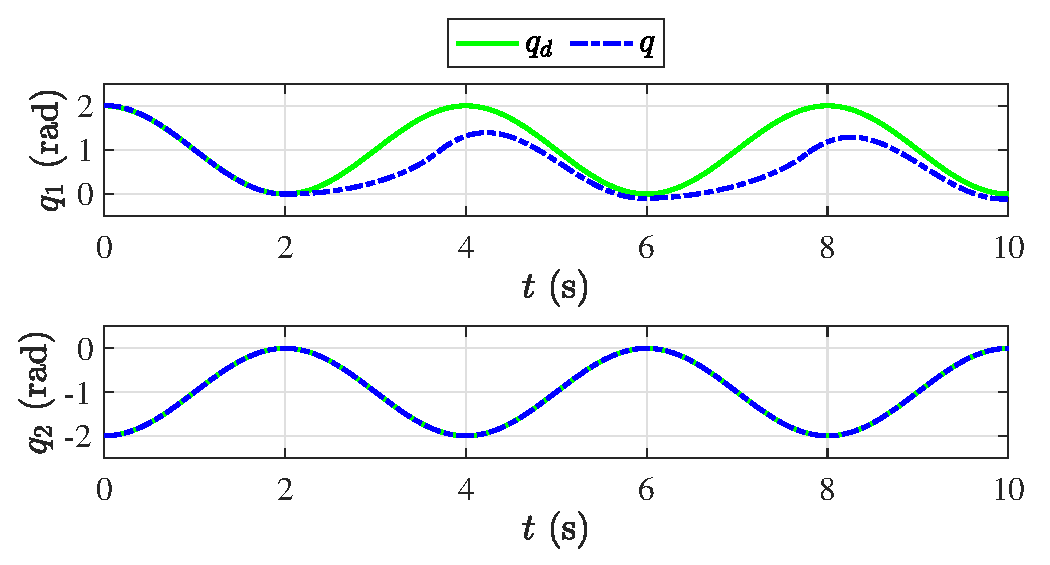
\includegraphics[width=0.8\linewidth]{imgs/Chap4/fig3.eps}%
        \label{chap4:fig:track_CM3}}
    \vfill
        \subfloat[CoNAC]{\includegraphics[width=0.8\linewidth]{imgs/Chap4/fig4.eps}%
        \label{chap4:fig:track_CoNAC}}
    \caption{Comparison of the tracking performance of DNN-BSC-A and CoNAC.}
    \label{chap4:fig:tracking2}
\end{figure}

% \begin{figure}[!t]
%     \centering
%         \subfloat[BSC]{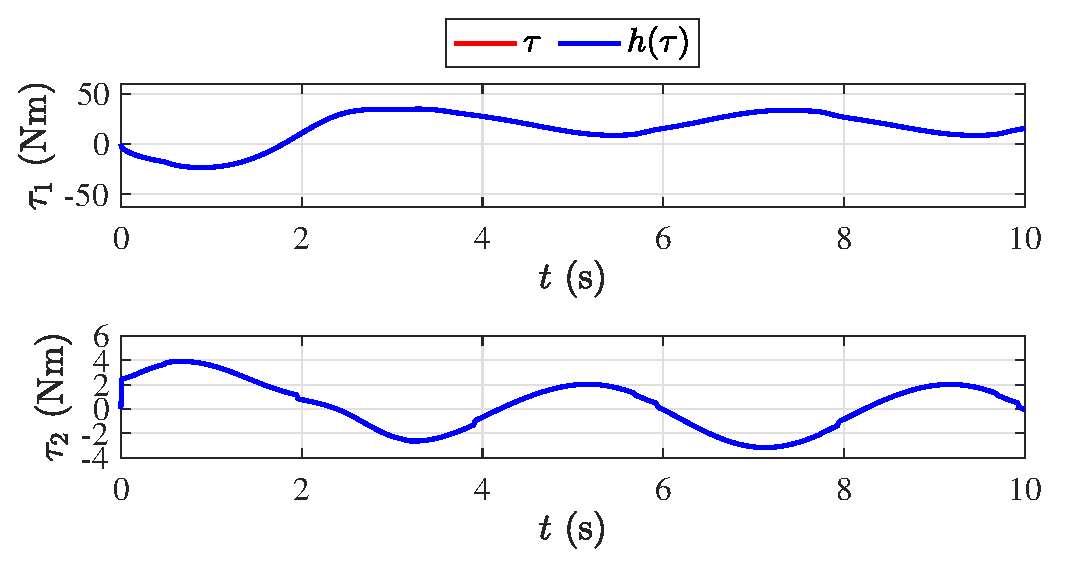
\includegraphics[width=0.49\linewidth]{imgs/Chap4/fig5.eps}%
%         \label{chap4:fig:control_CM1}}
%     \hfill
%         \subfloat[DNN-BSC]{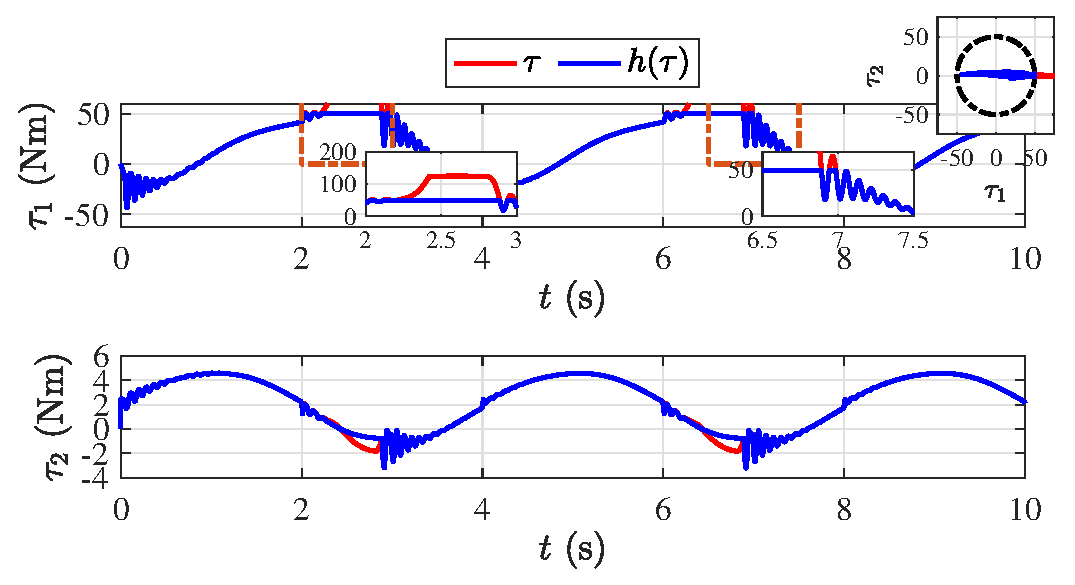
\includegraphics[width=0.49\linewidth]{imgs/Chap4/fig6.eps}%
%         \label{chap4:fig:control_CM2}}
%     \vfill
%         \subfloat[DNN-BSC-A]{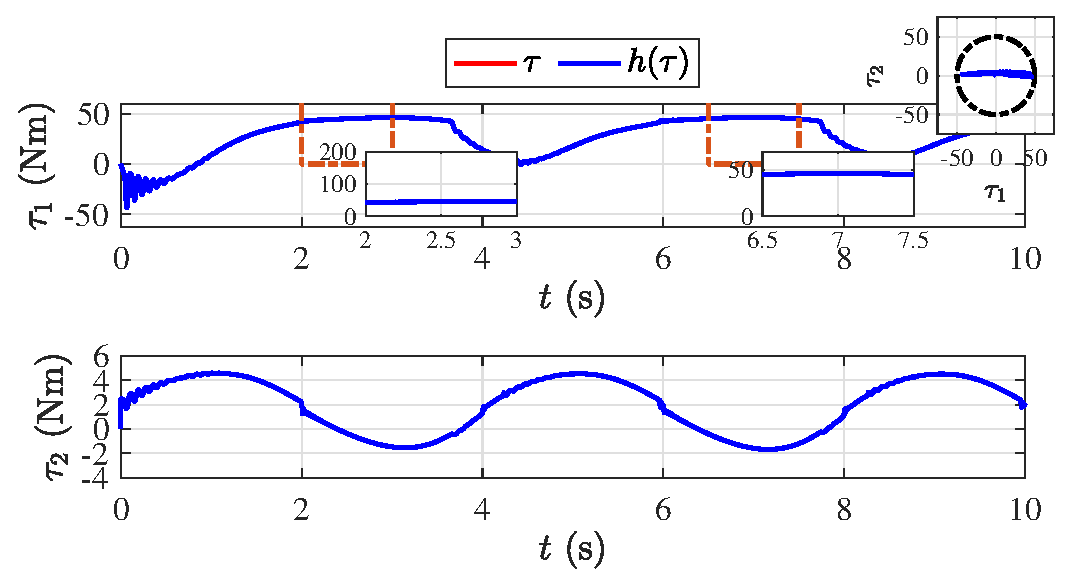
\includegraphics[width=0.49\linewidth]{imgs/Chap4/fig7.eps}%
%         \label{chap4:fig:control_CM3}}
%     \hfill
%         \subfloat[CoNAC]{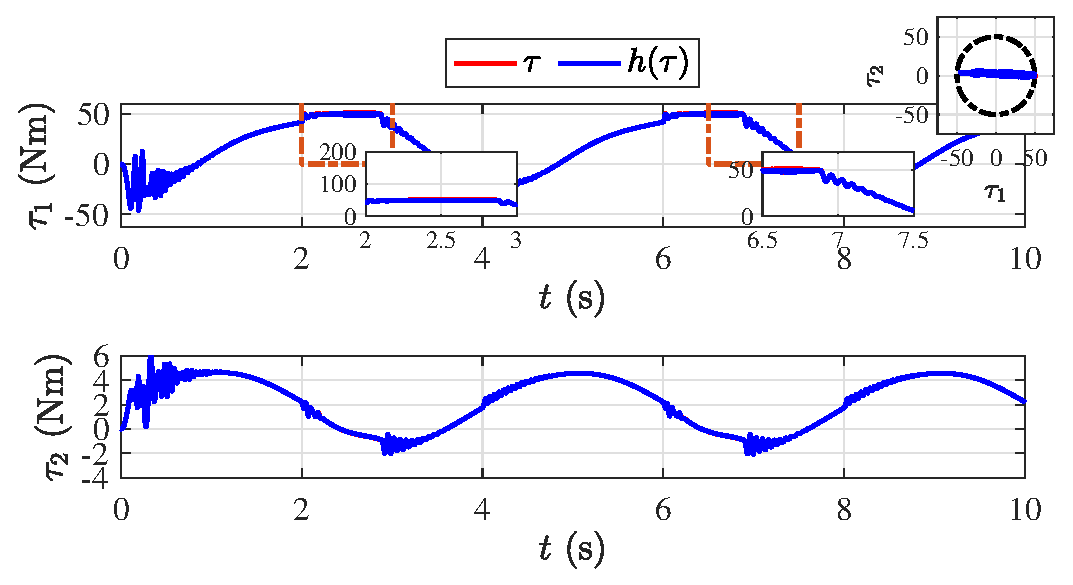
\includegraphics[width=0.49\linewidth]{imgs/Chap4/fig8.eps}%
%         \label{chap4:fig:control_CoNAC}}
%     \vfill
%     \caption{Comparison of the control input $\tau$ and the physically saturated control input $h(\tau)$ across the selected controllers.}
%     \label{chap4:fig:control}
% \end{figure}

\begin{figure}[!t]
    \centering
        \subfloat[BSC]{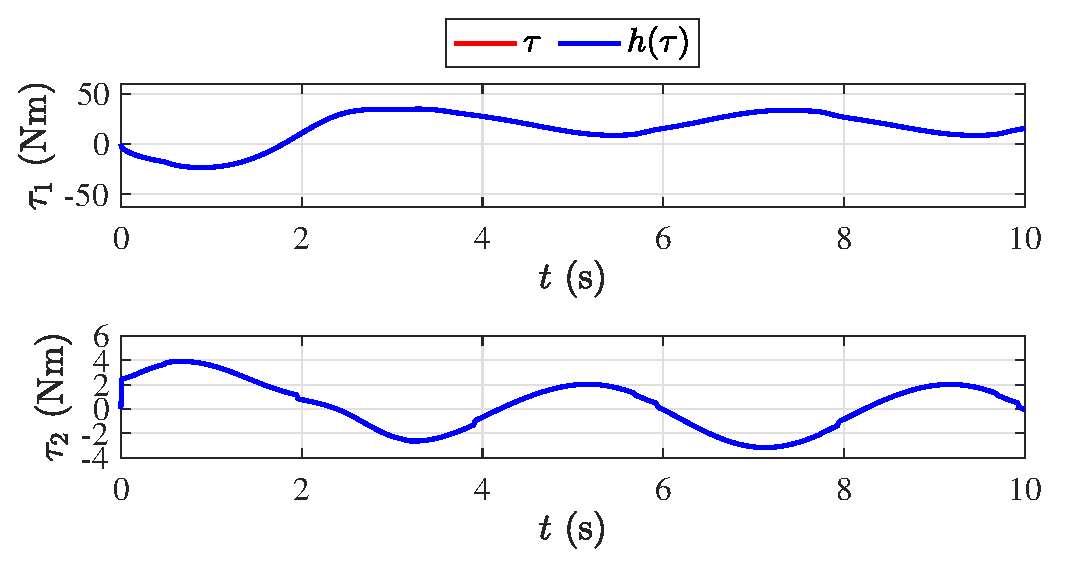
\includegraphics[width=0.8\linewidth]{imgs/Chap4/fig5.eps}%
        \label{chap4:fig:control_CM1}}
    \vfill
        \subfloat[DNN-BSC]{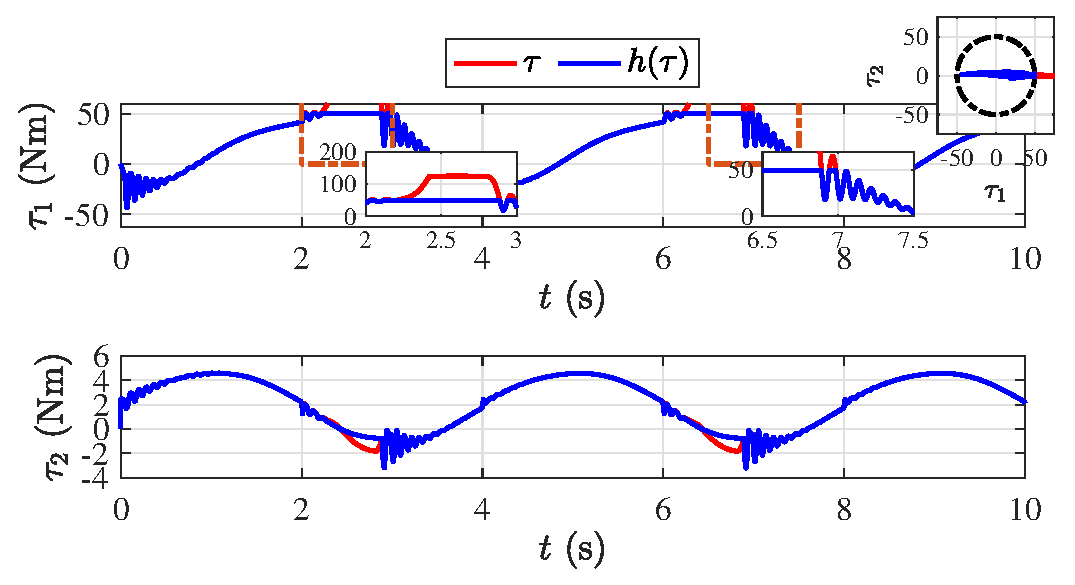
\includegraphics[width=0.8\linewidth]{imgs/Chap4/fig6.eps}%
        \label{chap4:fig:control_CM2}}
    \caption{Comparison of the control input $\tau$ and the physically saturated control input $h(\tau)$ of BSC and DNN-BSC.}
    \label{chap4:fig:control1}
\end{figure}

\begin{figure}[!t]
    \centering
        \subfloat[DNN-BSC-A]{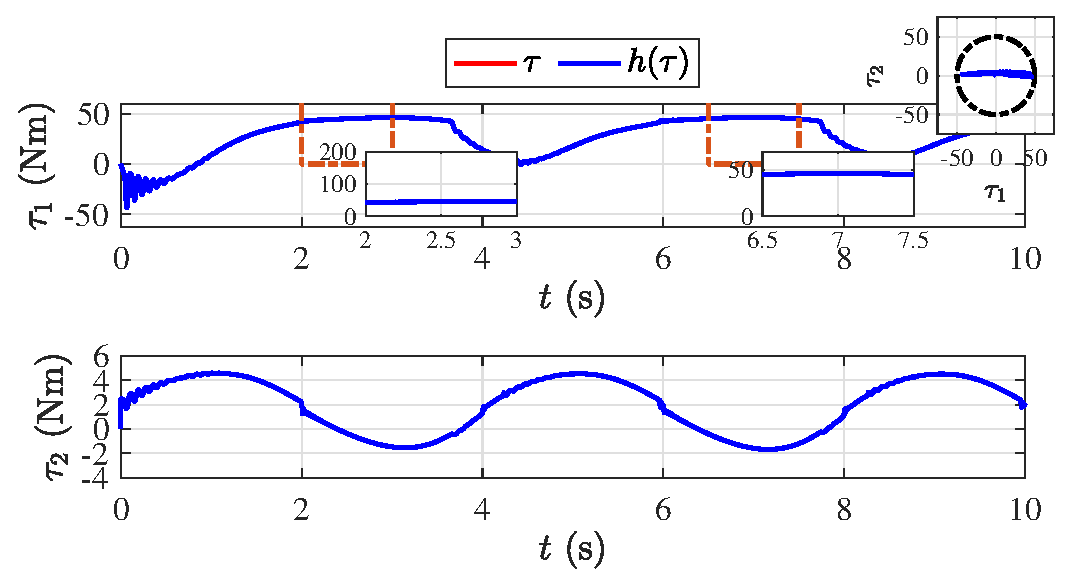
\includegraphics[width=0.8\linewidth]{imgs/Chap4/fig7.eps}%
        \label{chap4:fig:control_CM3}}
    \vfill
        \subfloat[CoNAC]{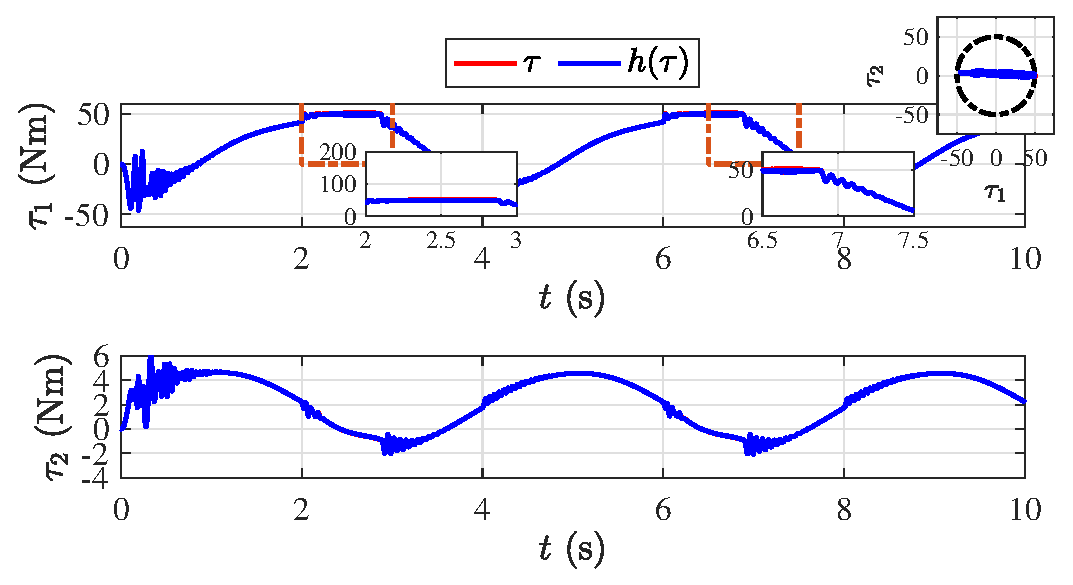
\includegraphics[width=0.8\linewidth]{imgs/Chap4/fig8.eps}%
        \label{chap4:fig:control_CoNAC}}
    \vfill
    \caption{Comparison of the control input $\tau$ and the physically saturated control input $h(\tau)$ of DNN-BSC-A and CoNAC.}
    \label{chap4:fig:control2}
\end{figure}

\begin{figure}[!t]
    \centering
    {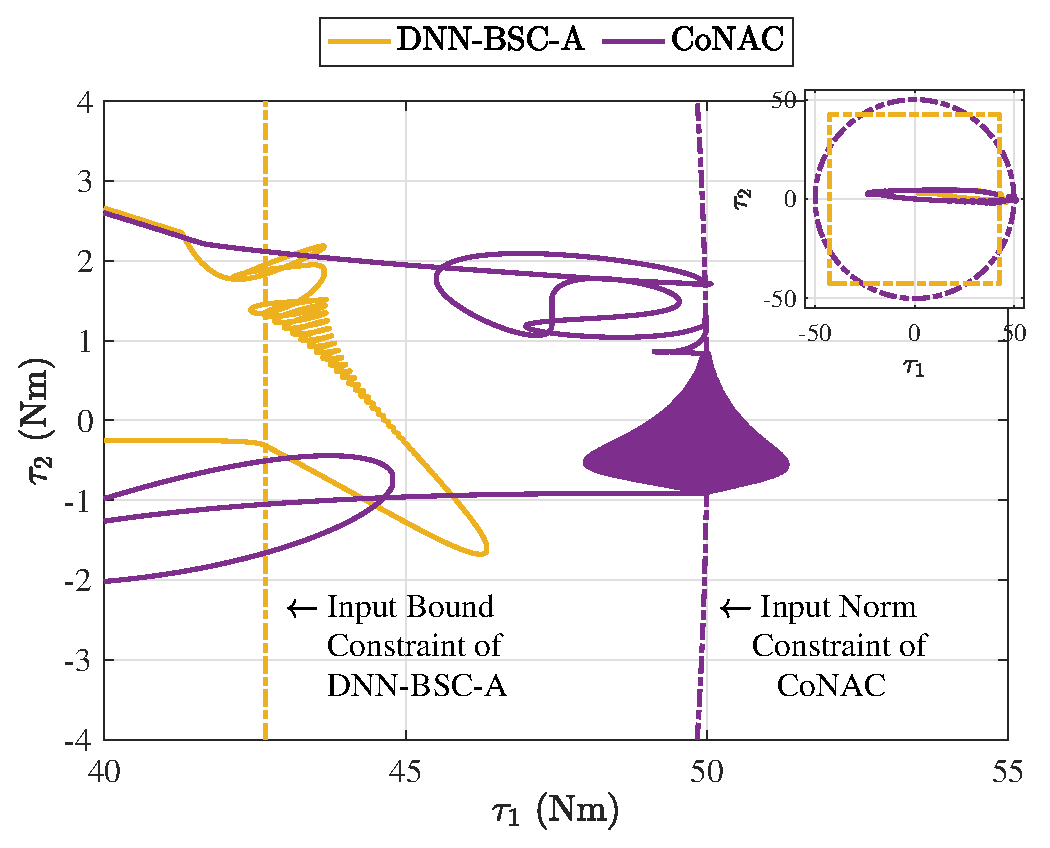
\includegraphics[width=0.85\linewidth]{imgs/Chap4/fig16.eps}
    \caption{Control input paths of DNN-BSC and CoNAC during the time interval from 5 s to 8 s.}
    \label{chap4:fig:control_ball}}
\end{figure}

% \begin{figure}[!t]
%     \centering
%         \subfloat[Multipliers of CoNAC]{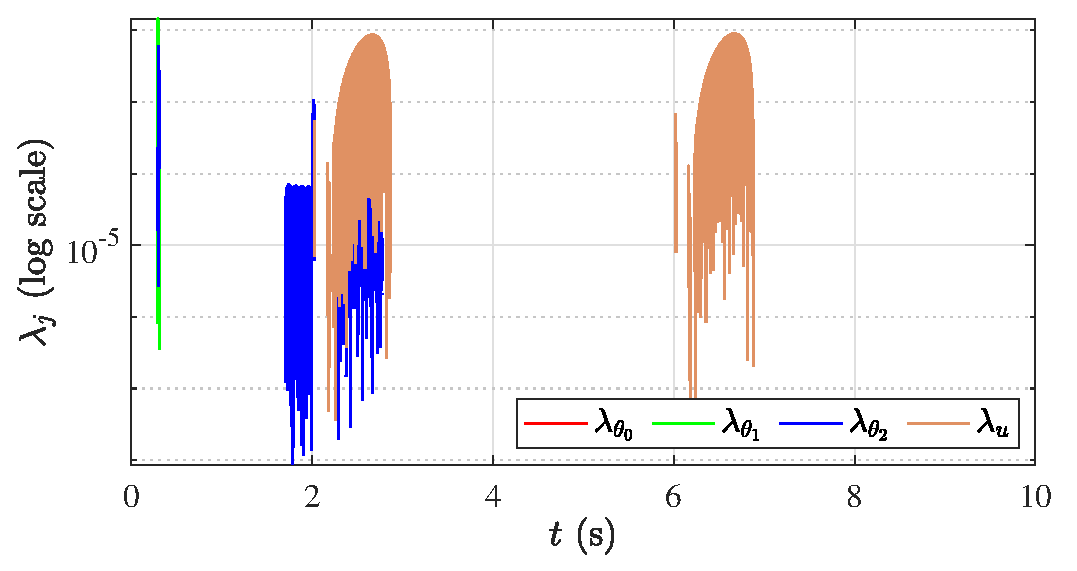
\includegraphics[width=0.49\linewidth]{imgs/Chap4/fig12.eps}%
%         \label{chap4:fig:multiplier}}
%     \hfill
%         \subfloat[Weight norms of DNN-BSC]{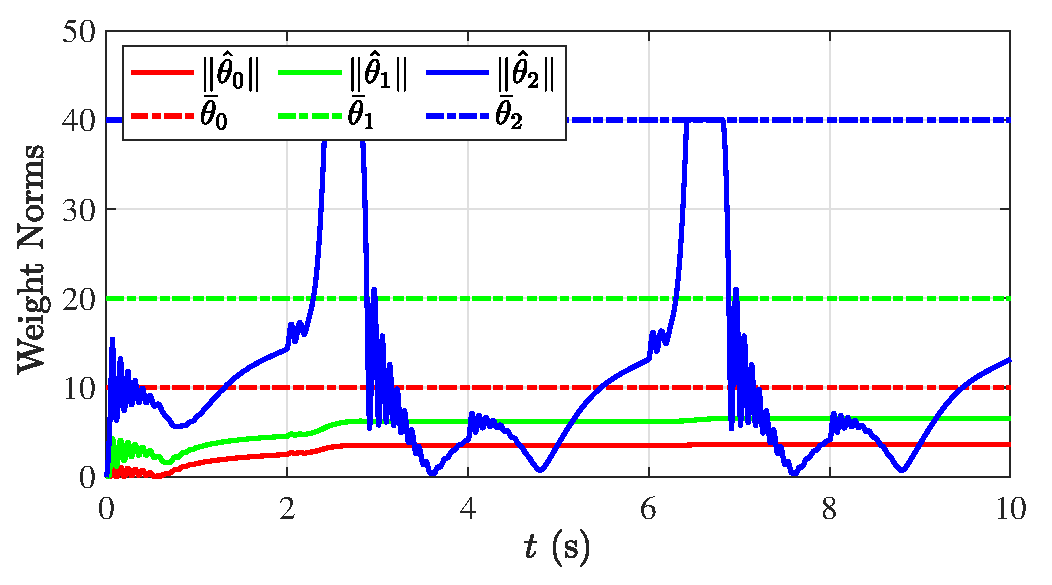
\includegraphics[width=0.49\linewidth]{imgs/Chap4/fig9.eps}%
%         \label{chap4:fig:weight_CM2}}
%     \vfill
%         \subfloat[Weight norms of DNN-BSC-A]{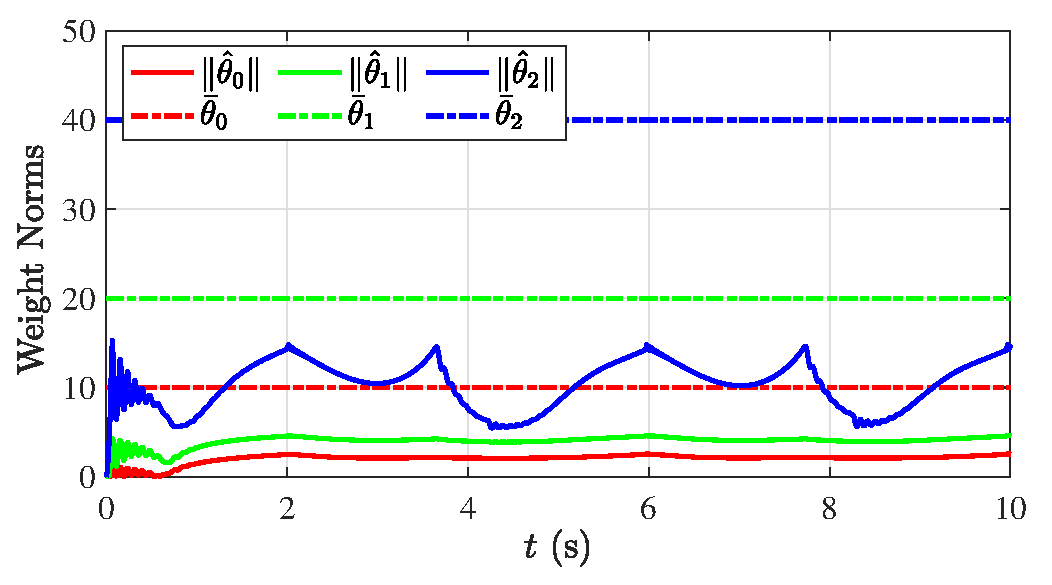
\includegraphics[width=0.49\linewidth]{imgs/Chap4/fig10.eps}%
%         \label{chap4:fig:weight_CM3}}
%     \hfill
%         \subfloat[Weight norms of CoNAC]{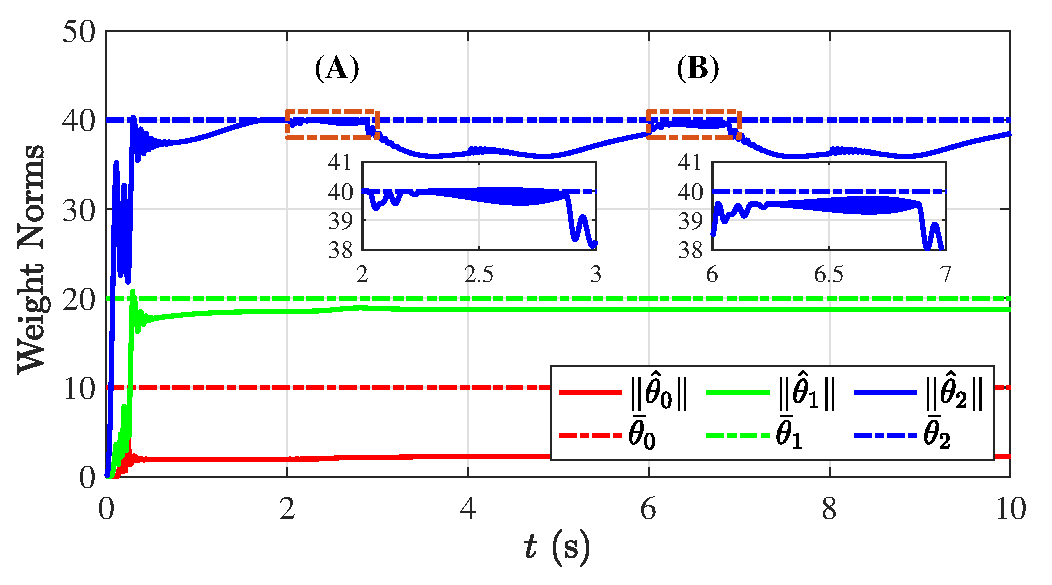
\includegraphics[width=0.49\linewidth]{imgs/Chap4/fig11.eps}%
%         \label{chap4:fig:weight_CoNAC}}       
%     \caption{Lagrange multipliers of CoNAC and weight norms of DNN-BSC, DNN-BSC-A, and CoNAC.}
%     \label{chap4:fig:weight_multiplier}
% \end{figure}

\begin{figure}[!t]
    \centering
        \subfloat[Weight norms of DNN-BSC]{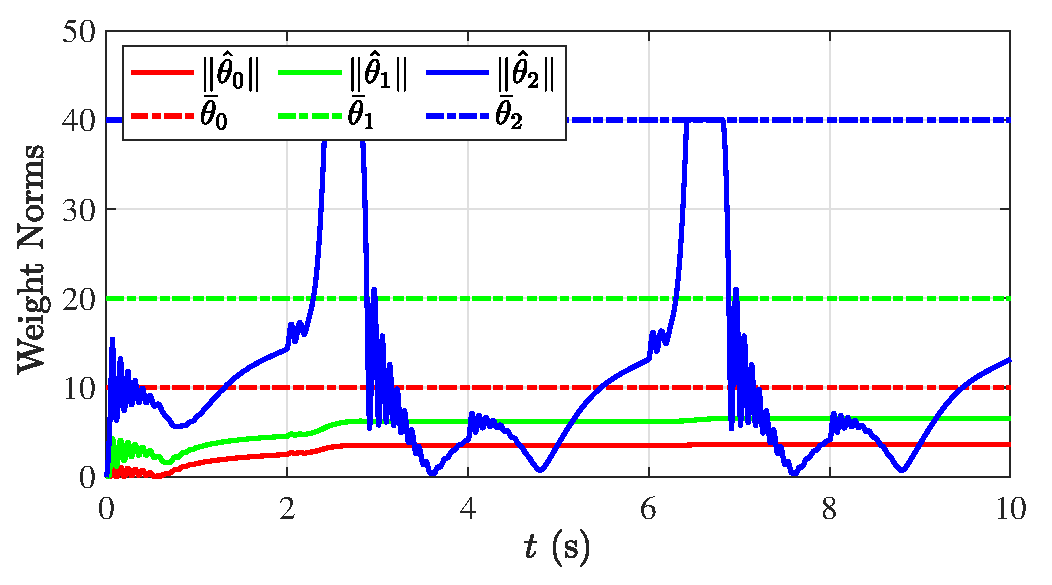
\includegraphics[width=0.8\linewidth]{imgs/Chap4/fig9.eps}%
        \label{chap4:fig:weight_CM2}}
    \vfill
        \subfloat[Weight norms of DNN-BSC-A]{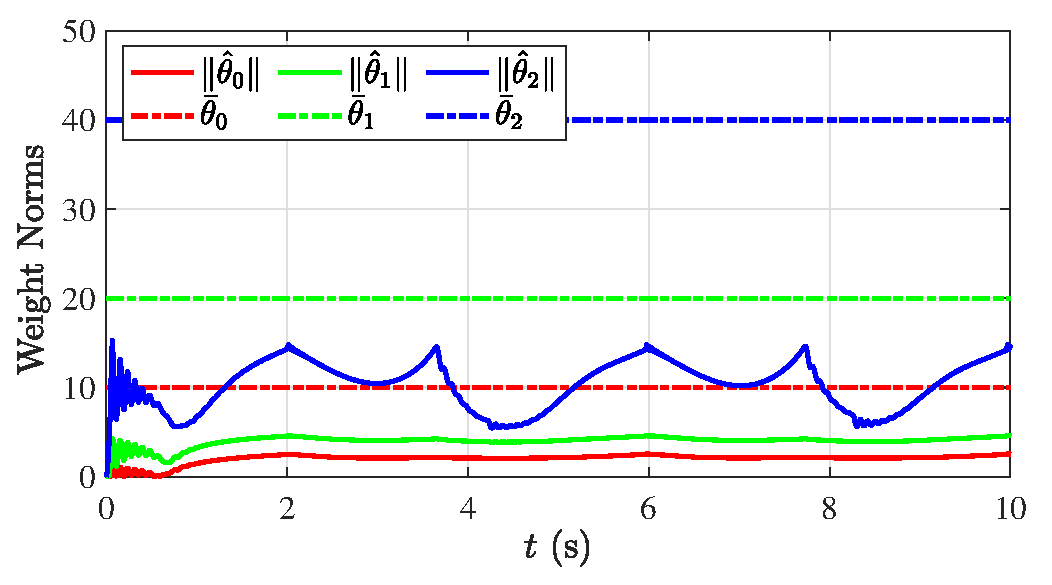
\includegraphics[width=0.8\linewidth]{imgs/Chap4/fig10.eps}%
        \label{chap4:fig:weight_CM3}}
    \caption{Weight norms of DNN-BSC and DNN-BSC-A.}
    \label{chap4:fig:weight_multiplier1}
\end{figure}

\begin{figure}[!t]
    \centering
        \subfloat[Multipliers of CoNAC]{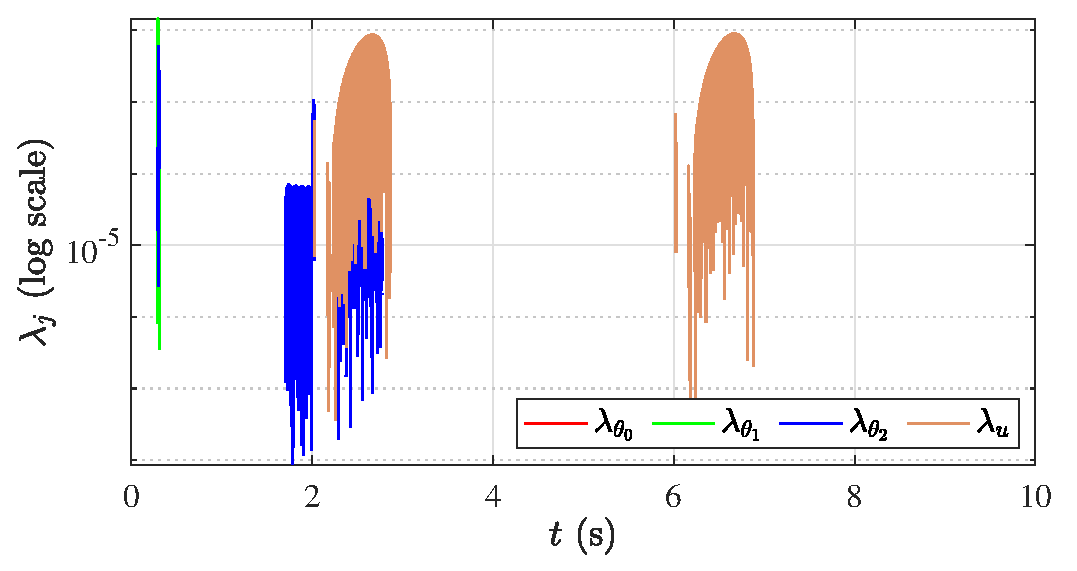
\includegraphics[width=0.8\linewidth]{imgs/Chap4/fig12.eps}%
        \label{chap4:fig:multiplier}}
    \vfill
        \subfloat[Weight norms of CoNAC]{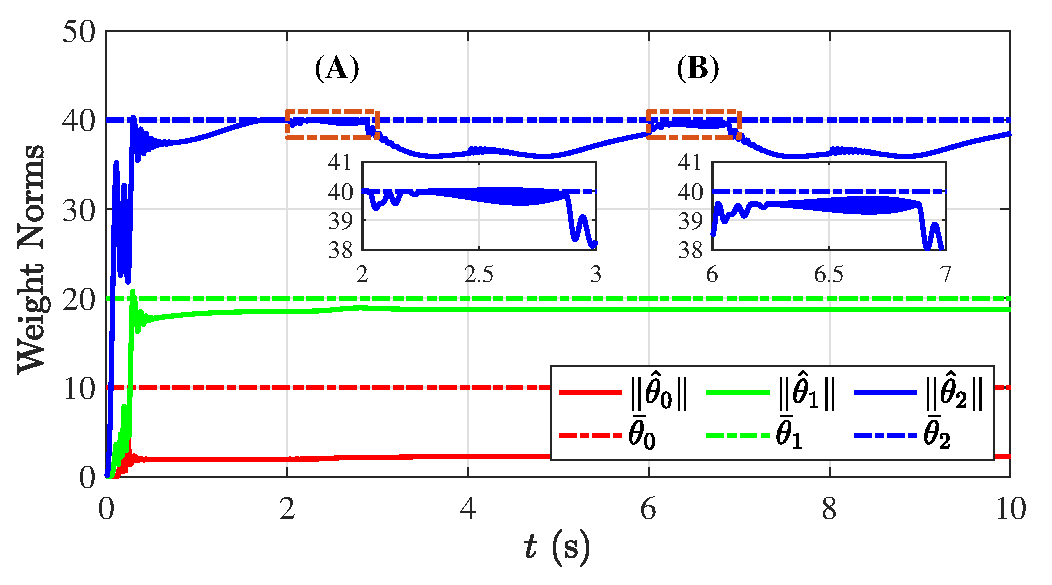
\includegraphics[width=0.8\linewidth]{imgs/Chap4/fig11.eps}%
        \label{chap4:fig:weight_CoNAC}}       
    \caption{Lagrange multipliers and weight norms CoNAC.}
    \label{chap4:fig:weight_multiplier2}
\end{figure}

% SIMULATION FIGURES
% **********************************************************

\subsection{Results}

\subsubsection{System Uncertainty Handling}

The tracking results of the selected controllers are shown in Fig.~\ref{chap4:fig:tracking1} and Fig.~\ref{chap4:fig:tracking2}.
To demonstrate the effectiveness of using DNNs for compensating the lumped system uncertainty function $f$, the gains ${k_q}$ and ${k_z}$ for BSC were intentionally selected as small values, resulting in a weak ability to handle these uncertainties. As a result,
%poor performance and sufficiently large values to satisfy \eqref{eq. ctrl stable condition}.
%the parameters of CM1 are poorly tuned, 
BSC failed to track the reference trajectory, as shown in Fig.~\ref{chap4:fig:track_CM1}.

By leveraging the DNN to compensate for the lumped system uncertainty within the BSC, DNN-BSC achieved improved tracking performance compared to BSC, as seen in Fig.~\ref{chap4:fig:track_CM2}. Fig.~\ref{chap4:fig:track_CM3} shows that DNN-BSC-A enhanced tracking performance for $q_2$, but tracking for $q_1$ remained unsatisfactory due to incomplete constraint handling, which will be discussed in detail in Section \ref{chap4:sec:sim:cstr input}.

Finally, CoNAC, which directly approximates the stabilizing control law along with the compensation term, demonstrated satisfactory tracking performance across both states, as illustrated in Fig.~\ref{chap4:fig:track_CoNAC}.

\subsubsection{Input Norm Constraint Handling} \label{chap4:sec:sim:cstr input}

The resulting control input $\tau$ and physically saturation control input $h(\tau)$ for the selected controllers are shown in Fig.~\ref{chap4:fig:control1} and Fig.~\ref{chap4:fig:control2}. As illustrated in Fig.~\ref{chap4:fig:control_CM1}, BSC did not violate the input norm constraint (\ie $\tau = h(\tau)$). However, in DNN-BSC, the added compensation term from the DNN caused violations of the input norm constraint (\ie $\tau > h(\tau)$) at several points; see Fig.~\ref{chap4:fig:control_CM2}. This failure to account for the input norm constraint led to oscillations in the control input $\tau$. The DNN adaptation process attempted to increase the weights to reduce the residual errors that were not constrained by saturation, but after saturation ceased, the control input had to rapidly adjust back to realistic levels, leading to oscillatory behavior. Such high-frequency oscillations may induce instability in the control system or cause fatigue in the actuators.

On the other hand, both DNN-BSC-A and CoNAC successfully handled their imposed input constraints, as shown in Fig.~\ref{chap4:fig:control_CM3} and Fig.~\ref{chap4:fig:control_CoNAC}, respectively, without causing notable oscillations in the control input $\tau$ even after the input constraint was activated. However, the tracking performance of DNN-BSC-A was lower than that of DNN-BSC and CoNAC, as the auxiliary system used in DNN-BSC-A approximated the input norm constraint with an input bound constraint, creating a rectangular constraint in the $\tau$-space (see Fig.~\ref{chap4:fig:control_ball}). In contrast, CoNAC satisfied the nonlinear input norm constraint and produced the physically maximum control input, resulting in improved tracking performance. 

It is also important to note that the control input trajectory in DNN-BSC-A depends on the dynamics of the auxiliary system. The auxiliary system regulates the violated control input after sufficient auxiliary state $\zeta$ is generated to compensate for the violation. This can be observed in Fig.~\ref{chap4:fig:control_ball}, where DNN-BSC-A exhibited minor violations of the input bound constraint. In contrast, CoNAC satisfied the constraint without being affected by such dynamics, as its Lagrange multiplier adjusted as soon as the constraint was violated.

\subsubsection{Weight Norm Constraint Handling}

The resulting weight norms of DNN-BSC, DNN-BSC-A, and CoNAC, along with the Lagrange multipliers of CoNAC, are shown in Fig.~\ref{chap4:fig:weight_multiplier1} and Fig.~\ref{chap4:fig:weight_multiplier2}. All three controllers—DNN-BSC, DNN-BSC-A, and CoNAC—maintained weight norms within the imposed weight norm constraints.

IN DNN-BSC, as shown in Fig.~\ref{chap4:fig:weight_CM2}, the weight norm of the last layer (\ie $\Vert {{{\hat \theta }_2}} \Vert$) fluctuated significantly over time, proportional to the control input norm. This is because the last layer’s weights directly determine the control input. When the control input violated the input norm constraint, the last layer’s weight norm hit the boundary and stayed there due to the projection operator. However, the projection operator only responded to violations without considering optimality or behavior.
%In the case of CM2 which does not consider the control input constraint, the weight norm of the last layer reaches the maximum weight norm value, when the control is saturated.
%It is because the weights get increased to produce larger control input to reduce the tracking error of $q_2$. (\ie the maximum magnitude of the control input depends on the weight norm of the last layer, since the activation function is bounded.)

In DNN-BSC-A, none of the weight norms reached their boundaries, as shown in Fig.~\ref{chap4:fig:weight_CM3}. This was due to the auxiliary system, where the auxiliary state $\zeta$ reduced the control input, ensuring it stayed within the input constraint.

In CoNAC, all weight norms complied with the imposed constraints through the constrained optimization approach, as illustrated in Fig.\ref{chap4:fig:weight_CoNAC}. When any weight norm approached its upper limit, the Lagrange multiplier was promptly activated to steer the weight adaptation direction towards a constraint-satisfactory point (see Fig.\ref{chap4:fig:multiplier}). Notably, the weight norms of the first and second layers ($\Vert {{{\hat \theta }_0}} \Vert$ and $\Vert {{{\hat \theta }_1}} \Vert$) remained nearly constant throughout the control period. The weight norm of the last layer $\Vert {{{\hat \theta }_2}} \Vert$ stabilized within the upper bound by around 6.5 seconds (see Fig.~\ref{chap4:fig:weight_CoNAC} (B)), coinciding with the activation of the input norm constraint. This quasi-static behavior of the weight norm (\ie $d{\hat\theta}/dt=-\alpha\partial L/\partial \hat\theta \approx 0$) along with the quasi-static behavior of the Lagrange multipliers (\ie $\dot\lambda_j = \beta_j c_j \approx 0$) implies that the weights were updated near the KKT conditions, signifying local optimality in CoNAC. However, at around 2.5 seconds (see Fig.~\ref{chap4:fig:weight_CoNAC} (A)), the weight norm of the last layer reached the upper limit earlier, despite similar control conditions as the case at 6.5 seconds. This earlier saturation likely occurred because the optimization process had not yet fully converged to the optimal weight values.

The overall weight norms of CoNAC were larger than those of DNN-BSC and DNN-BSC-A, since CoNAC approximated the entire stabilizing control law, whereas DNN-BSC and DNN-BSC-A only approximated the system uncertainty term within the BSC framework.

%%%%%%%%%%%%%%%%%%%%%%%%%%%%%%%%
\section{Conclusion} 
%%%%%%%%%%%%%%%%%%%%%%%%%%%%%%%%

In this chapter, a Constrained Optimization-based Neuro-Adaptive Controller \allowbreak (CoNAC) for the uncertain Euler-Lagrange system is extended to address both weight norm and input constraints using deep neural network (DNN).
The adaptation law is derived through a rigorous optimization framework. 
The stability of the proposed controller was analyzed using Lyapunov theory, ensuring that the system maintained bounded tracking and estimation errors under real-time adaptation.

The controller effectively incorporated both the input (bound or norm) constraint and the weight norm constraint, ensuring that both actuator limitations and neural network weights were kept within predefined bounds. 
By formulating these constraints as part of the optimization process, CoNAC ensured that the weights converged in a way that satisfied the Karush-Kuhn-Tucker (KKT) conditions, guaranteeing optimality and stability.

Simulation results validated the superior performance of CoNAC compared to conventional methods, such as DNN-BSC and DNN-BSC-A. 
CoNAC not only handled complex input constraints but also managed the weight norm constraints rigorously, leading to improved tracking accuracy and stability without notable oscillations.


\end{spacing}

      
%%%%%%%%%%%%%%%%%%%%%%%%%%%%%%%%%%%%
% Chapter 5 
%%%%%%%%%%%%%%%%%%%%%%%%%%%%%%%%%%%%

% \begin{spacing}{2.0} % double spacing
\begin{spacing}{1.3} % double spacing
%%%%%%%%%%%%%%%%%%%%%%%%%%%%%%%%
% Chap 5. Conclusion and Future Work
%%%%%%%%%%%%%%%%%%%%%%%%%%%%%%%%

\chapter{Conclusion and Future Work} \label{chapter5}

In this thesis, the Constrained Optimization-based Neuro-Adaptive Controller (Co\allowbreak NAC) for uncertain Euler-Lagrange systems is presented. 
The two simulation validations showed that the CoNAC can satisfy the imposed constraints regarding boundedness of neural network's (NN's) weights and control input saturation, while achieving the desired tracking performance.

However, neuro-adaptive control (NAC) methods including CoNAC have several limitations to be referred as deep learning-based controller.
First, NAC methods adapts their weights to reduce objective function using current tracking error. 
This means online implementation is required to train the NNs since the tracking error is dependent on the current NNs' weights.
Moreover, for the same reason, the NNs cannot be trained offline.
Second, the gradient vanishing problem still exists in the train process of the NNs.
To overcome this issue, simply ReLU activation function can be used.
However, the stability should be examined rigorously, since this activation function is unbounded.

The following future works are suggested to tackle above limitations.
First, reinforcement learning (RL) approach can be used, since training NNs to minimize objective function is similar as RL which trains to maximize the expected reward with respect to tracking error.
There are some literature based on optimal control theory \cite{RN119,RN120,RN121}.
They approximate optimal control law which is ideally obtained using Hamilton-Jacobi-Bellman framework.
Second, if the offline adaptation is available, stochastic problem formulation can be used to theoretically utilize novel deep learning methods.
Since the recent deep learning methods are based on stochastic methods (\eg, stochastic gradient descent (SGD), drop out, $L_2$-regularization), stochastic stability analysis should be conducted.
The stability analysis of system which uses stochastic neural network is introduced in \cite{RN122,RN123}.
Third, other novel constrained optimization methods can be used to solve gradient vanishing issue.
Except gradient descent-like methods, the existing methods to overcome gradient vanishing issue using constrained optimization approach such as the augmented Lagrangian method (ALM) \cite{RN62} and the alternating direction method of multipliers (ADMM) \cite{RN98, RN94} are introduced.
These methods transform the NN's architecture of the NNs to equality constraints and optimize each layer's weights and output of activation functions.


      
\end{spacing}
      
%%%%%%%%
% Add more chapters if you wants
%%%%%%%%


%---------
% summary
%---------
\begin{spacing}{2.0}

\summary

In this thesis, the Constrained Optimization-based Neuro-Adaptive Controller \allowbreak (CoNAC) for uncertain Euler-Lagrange systems is presented. 
The neural network (NN) in the CoNAC is used to approximate the uncertainties of the system.
Therefore, any prior knowledge of the system uncertainties is not required.
To derive the adaptation laws of NN's weights and Lagrange multipliers, the control problem is formulated as a constrained optimization problem.
Satisfactions of the boundedness of the weights and control input saturation are transformed into constraints in the constrained optimization problem.
Using the problem, the adaptation laws are derived based on corresponding Lagrangian function.
The stability of the CoNAC is analyzed using the Lyapunov stability theorem.
Two simulation validations are conducted using a two-link manipulator model to validate the CoNAC.
The simulations demonstrated that the CoNAC can achieve the sufficient tracking performance while satisfying the constraints on the weights and control input saturation.


\end{spacing}

%-----------------------------------------------------------------------
% This is the end of the main thesis body.

%-----------------------------------------------------------------------
% Input the list of references.
\bibliographystyle{ieeetr}
\bibliography{biblist}

%%%%%%%%%%%%%%%%%%%%%%%%%%%%%%%%%%%%%%%%%%%%%%%%
% Appendix
% You can comment out if you do not need appendix
%%%%%%%%%%%%%%%%%%%%%%%%%%%%%%%%%%%%%%%%%%%%%%%%
% \begin{spacing}{2.0}
% 
%%%%%%%%%%%%%%%%%%%%%%%%%%%%%%%%%%%%%%%%%%%%%%%%
% Appendix
%%%%%%%%%%%%%%%%%%%%%%%%%%%%%%%%%%%%%%%%%%%%%%%%

%\appendixpage
\appendix

\chapter{Abbreviations}
%%% define some Abbreviations
\text{ } \text{ }  \textbf{GIST} \text{ } \text{ } Gwangju Institute of Science and Technology

\textbf{EECS}  \text{ } \text{ } Electrical Engineering and Computer Science

\textbf{YOLO}  \text{ } \text{ } You Only Live Once



\chapter{More appendix}

You can add more appendices.
% \end{spacing}

%-----------------------------------------------------------------------
% Acknowledgements
% Insert the text between \begin{acknowledgements} and \end{acknowledgements}.
% You can either write the abstract directly here or import a file using the \input command.

%%%%%%%%%%%%%%%%%%%%%%%%%%%%%%%%%%%%%%%%%%
% Acknowledgements by Korean
%%%%%%%%%%%%%%%%%%%%%%%%%%%%%%%%%%%%%%%%%%
\begin{acknowledgements}
\begin{spacing}{2.0}
%%%%%%%%%%%%%%%%%%%%%%%%%%%%%%%%%%%%%%
% Acknowledgements of the thesis in English
%%%%%%%%%%%%%%%%%%%%%%%%%%%%%%%%%%%%%%

먼저, 본 석사 학위 논문을 작성하는 데 아낌없는 의견 교류와 조언을 해주신 최경환 지도 교수님께 감사의 말씀 드립니다.
교수님께서 석사과정 학생인 저에게 제공한 과분한 연구적 자유와 지원이 없었다면 여기까지 제 생각을 확장할 수 없었을 것입니다.
아울러 모자란 학위 논문을 심사하여 주신 최경환 교수님을 비롯한 안효성 교수님과 허필원 교수님께 감사드립니다.
교수님들께서 지적하여 주신 부분을 보완하여 완성도를 높일 수 있었습니다.

또한, 이 논문은 부모님과 하나뿐인 형제의 무한한 사랑과 무언의 기다림, 지지가 없었다면 존재하지 않았을 것입니다.
단거리의 미래도 예측할 수 없는 인생에서 언제나 돌아갈 수 있는 든든하고 따뜻한 가족이 있다는 것은 큰 행운이라고 생각합니다.
그렇기에, 제 생각을 부족함 없이 써 내려간 이 논문의 마지막 한 장의 한 문단을 빌려, 그동안 잘 표현하지 못한 부모님과 형제에 감사의 말을 전합니다.

그리고, 옆에서 함께 고민하고 논의하여 익숙지 않은 주제와 관점을 제공해 주고 정신적 버팀목이 되어준 연구실 동료들에게 감사드립니다.
특별히, 연구 접근에 대하여 여러 생각을 하게 해준 승훈이 형, 논문 작업을 도와준 동화 형과 지윤이, 언제나 편하게 대할 수 있는 재준이, 그리고 마음속 깊은 의견을 나눌 수 있는 민석이에게 감사드립니다.
마지막으로, 드넓은 학술의 우주에서 아주 조그마한 탐색을 할 수 있도록 그 토대와 동기를 마련해준 선대 연구자들에게 감사드립니다.
그 외, 언급되지 않은 이 논문을 작성하는 데 도움을 주신 모든 분에게 감사드립니다.
\end{spacing}
\end{acknowledgements}


%-----------------------------------------------------------------------
% Input the curriculum vitae.
% You may add as many lines as you need using the syntax of the \item command shown below.
%-----------------------------------------------------------------------



%\input Vitae2.0.tex
%\input thesis-publications.tex

% Insert activity if you have.
%\activity
%Activity Activity Activity Activity Activity Activity Activity Activity
%Activity Activity Activity Activity Activity Activity Activity Activity

% Insert awards if you have.

%-----------------------------------------------------------------------
% This is the end of the thesis.
%
\end{document}
